\documentclass[]{book}
\usepackage{lmodern}
\usepackage{amssymb,amsmath}
\usepackage{ifxetex,ifluatex}
\usepackage{fixltx2e} % provides \textsubscript
\ifnum 0\ifxetex 1\fi\ifluatex 1\fi=0 % if pdftex
  \usepackage[T1]{fontenc}
  \usepackage[utf8]{inputenc}
\else % if luatex or xelatex
  \ifxetex
    \usepackage{mathspec}
  \else
    \usepackage{fontspec}
  \fi
  \defaultfontfeatures{Ligatures=TeX,Scale=MatchLowercase}
\fi
% use upquote if available, for straight quotes in verbatim environments
\IfFileExists{upquote.sty}{\usepackage{upquote}}{}
% use microtype if available
\IfFileExists{microtype.sty}{%
\usepackage{microtype}
\UseMicrotypeSet[protrusion]{basicmath} % disable protrusion for tt fonts
}{}
\usepackage[margin=1in]{geometry}
\usepackage{hyperref}
\PassOptionsToPackage{usenames,dvipsnames}{color} % color is loaded by hyperref
\hypersetup{unicode=true,
            colorlinks=true,
            linkcolor=Maroon,
            citecolor=Blue,
            urlcolor=blue,
            breaklinks=true}
\urlstyle{same}  % don't use monospace font for urls
\usepackage{longtable,booktabs}
\usepackage{graphicx,grffile}
\makeatletter
\def\maxwidth{\ifdim\Gin@nat@width>\linewidth\linewidth\else\Gin@nat@width\fi}
\def\maxheight{\ifdim\Gin@nat@height>\textheight\textheight\else\Gin@nat@height\fi}
\makeatother
% Scale images if necessary, so that they will not overflow the page
% margins by default, and it is still possible to overwrite the defaults
% using explicit options in \includegraphics[width, height, ...]{}
\setkeys{Gin}{width=\maxwidth,height=\maxheight,keepaspectratio}
\IfFileExists{parskip.sty}{%
\usepackage{parskip}
}{% else
\setlength{\parindent}{0pt}
\setlength{\parskip}{6pt plus 2pt minus 1pt}
}
\setlength{\emergencystretch}{3em}  % prevent overfull lines
\providecommand{\tightlist}{%
  \setlength{\itemsep}{0pt}\setlength{\parskip}{0pt}}
\setcounter{secnumdepth}{5}
% Redefines (sub)paragraphs to behave more like sections
\ifx\paragraph\undefined\else
\let\oldparagraph\paragraph
\renewcommand{\paragraph}[1]{\oldparagraph{#1}\mbox{}}
\fi
\ifx\subparagraph\undefined\else
\let\oldsubparagraph\subparagraph
\renewcommand{\subparagraph}[1]{\oldsubparagraph{#1}\mbox{}}
\fi

%%% Use protect on footnotes to avoid problems with footnotes in titles
\let\rmarkdownfootnote\footnote%
\def\footnote{\protect\rmarkdownfootnote}

%%% Change title format to be more compact
\usepackage{titling}

% Create subtitle command for use in maketitle
\newcommand{\subtitle}[1]{
  \posttitle{
    \begin{center}\large#1\end{center}
    }
}

\setlength{\droptitle}{-2em}

  \title{}
    \pretitle{\vspace{\droptitle}}
  \posttitle{}
    \author{}
    \preauthor{}\postauthor{}
    \date{}
    \predate{}\postdate{}
  
\usepackage{booktabs}
\usepackage{amsthm}
\makeatletter
\def\thm@space@setup{%
  \thm@preskip=8pt plus 2pt minus 4pt
  \thm@postskip=\thm@preskip
}
\makeatother

\begin{document}

\newcommand{\HRule}{\rule{\linewidth}{0.5mm}}

\pagenumbering{gobble}

%\begin{titlepage}
\begin{center}

\textsc{\LARGE
\strong{H}uman-\strong{P}lant \strong{C}oevolution model
} \\[1cm]
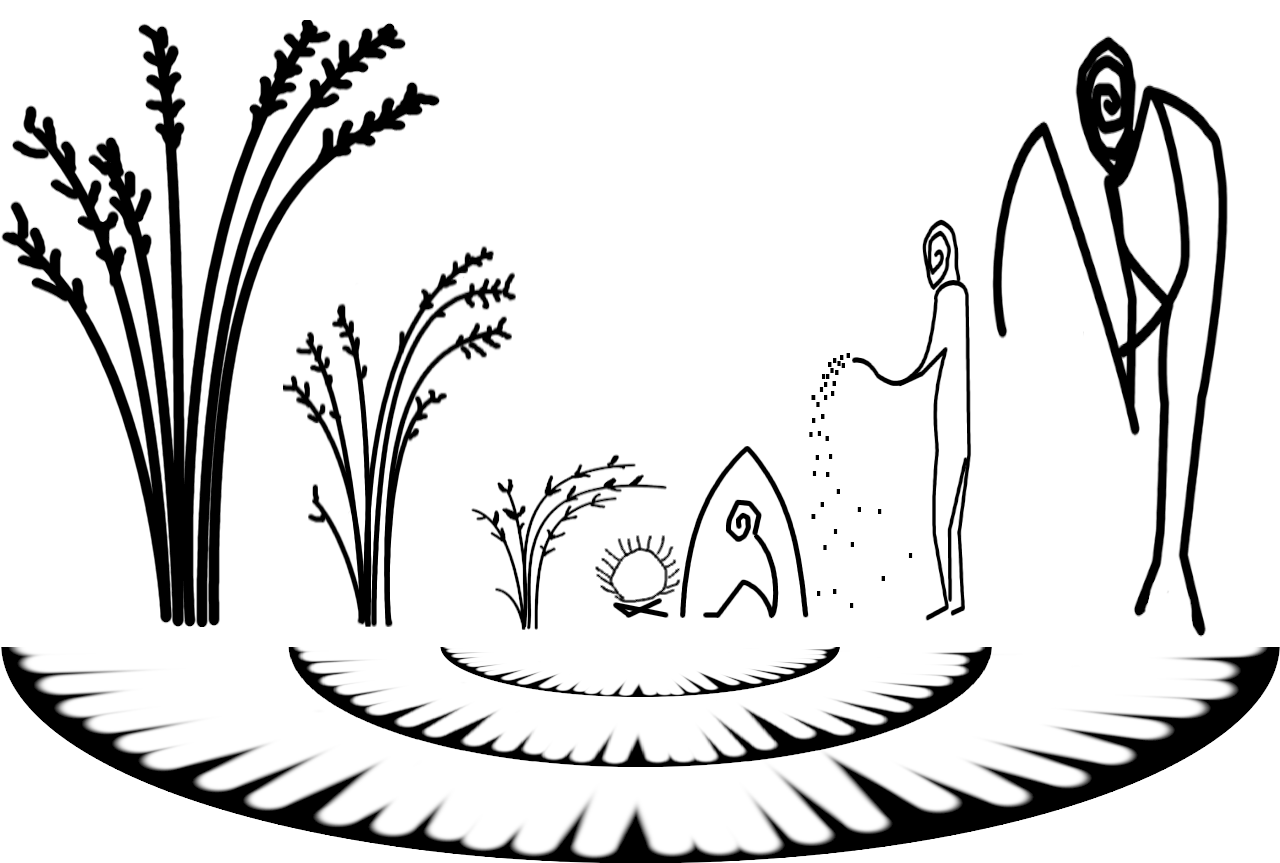
\includegraphics[width=\textwidth]{images/hpcModel-logo_v2.png}
\\[1.5cm]
\HRule \\[0.4cm]
{ \huge General exploration and parameter sensitivity analysis \\[0.15cm] }
\HRule \\[1.5cm]
Andreas Angourakis \& Jon\`{a}s Alcaina
\\[1cm]
\today \\ [1cm]

\end{center}
% \end{titlepage}

\newpage
\pagenumbering{arabic}

{
\hypersetup{linkcolor=black}
\setcounter{tocdepth}{1}
\tableofcontents
}
\hypertarget{model-overview}{%
\chapter{Model overview}\label{model-overview}}

The Human-Plant Coevolution (HPC) model represents the dynamics of coevolution between a human and a plant population. The model consists of an ecological positive feedback system (mutualism), which can be reinforced by positive evolutionary feedback (coevolution). The model is the result of wiring together relatively simple simulation models of population ecology and evolution, through a computational implementation in R.

\textbf{\emph{Parameters}}

\begin{longtable}[]{@{}lll@{}}
\toprule
\begin{minipage}[b]{0.27\columnwidth}\raggedright
R notation\strut
\end{minipage} & \begin{minipage}[b]{0.25\columnwidth}\raggedright
Math notation\strut
\end{minipage} & \begin{minipage}[b]{0.40\columnwidth}\raggedright
Description\strut
\end{minipage}\tabularnewline
\midrule
\endhead
\begin{minipage}[t]{0.27\columnwidth}\raggedright
\texttt{iniH}, \texttt{iniP}\strut
\end{minipage} & \begin{minipage}[t]{0.25\columnwidth}\raggedright
\(ini_{H},\,ini_{P}\)\strut
\end{minipage} & \begin{minipage}[t]{0.40\columnwidth}\raggedright
initial populations of humans and plants\strut
\end{minipage}\tabularnewline
\begin{minipage}[t]{0.27\columnwidth}\raggedright
\texttt{n.H}, \texttt{n.P}\strut
\end{minipage} & \begin{minipage}[t]{0.25\columnwidth}\raggedright
\(n_{H},\,n_{P}\)\strut
\end{minipage} & \begin{minipage}[t]{0.40\columnwidth}\raggedright
number of types of humans and plants\strut
\end{minipage}\tabularnewline
\begin{minipage}[t]{0.27\columnwidth}\raggedright
\texttt{v.H}, \texttt{v.P}\strut
\end{minipage} & \begin{minipage}[t]{0.25\columnwidth}\raggedright
\(v_{H},\,v_{P}\)\strut
\end{minipage} & \begin{minipage}[t]{0.40\columnwidth}\raggedright
level of undirected variation in humans and plants\strut
\end{minipage}\tabularnewline
\begin{minipage}[t]{0.27\columnwidth}\raggedright
\texttt{r.H}, \texttt{r.P}\strut
\end{minipage} & \begin{minipage}[t]{0.25\columnwidth}\raggedright
\(r_{H},\,r_{P}\)\strut
\end{minipage} & \begin{minipage}[t]{0.40\columnwidth}\raggedright
intrinsic growth rates for human and plant populations\strut
\end{minipage}\tabularnewline
\begin{minipage}[t]{0.27\columnwidth}\raggedright
\texttt{mU.PnH}\strut
\end{minipage} & \begin{minipage}[t]{0.25\columnwidth}\raggedright
\(\bar{U}_{P_{n}H}\)\strut
\end{minipage} & \begin{minipage}[t]{0.40\columnwidth}\raggedright
utility per capita \textbf{of} type n plants \textbf{to} humans\strut
\end{minipage}\tabularnewline
\begin{minipage}[t]{0.27\columnwidth}\raggedright
\texttt{mU.HnP}\strut
\end{minipage} & \begin{minipage}[t]{0.25\columnwidth}\raggedright
\(\bar{U}_{H_{n}P}\)\strut
\end{minipage} & \begin{minipage}[t]{0.40\columnwidth}\raggedright
utility per capita \textbf{of} type n humans \textbf{to} plants\strut
\end{minipage}\tabularnewline
\begin{minipage}[t]{0.27\columnwidth}\raggedright
\texttt{mU.P1H}\strut
\end{minipage} & \begin{minipage}[t]{0.25\columnwidth}\raggedright
\(\bar{U}_{P_{1}H}\)\strut
\end{minipage} & \begin{minipage}[t]{0.40\columnwidth}\raggedright
utility per capita \textbf{of} type 1 plants \textbf{to} humans\strut
\end{minipage}\tabularnewline
\begin{minipage}[t]{0.27\columnwidth}\raggedright
\texttt{mU.H1P}\strut
\end{minipage} & \begin{minipage}[t]{0.25\columnwidth}\raggedright
\(\bar{U}_{H_{1}P}\)\strut
\end{minipage} & \begin{minipage}[t]{0.40\columnwidth}\raggedright
utility per capita \textbf{of} type 1 humans \textbf{to} plants\strut
\end{minipage}\tabularnewline
\begin{minipage}[t]{0.27\columnwidth}\raggedright
\texttt{U.bH1}\strut
\end{minipage} & \begin{minipage}[t]{0.25\columnwidth}\raggedright
\(U_{bH_{1}}\)\strut
\end{minipage} & \begin{minipage}[t]{0.40\columnwidth}\raggedright
utility \textbf{of} other resources \textbf{to} humans of type 1 (the baseline carrying capacity for humans of type 1, i.e.~independent of HP relationship)\strut
\end{minipage}\tabularnewline
\begin{minipage}[t]{0.27\columnwidth}\raggedright
\texttt{U.bP1}\strut
\end{minipage} & \begin{minipage}[t]{0.25\columnwidth}\raggedright
\(U_{bP_{1}}\)\strut
\end{minipage} & \begin{minipage}[t]{0.40\columnwidth}\raggedright
utility \textbf{of} non-anthropic space \textbf{to} type 1 plants (the baseline carrying capacity for plants of type 1, i.e.~independent of HP relationship)\strut
\end{minipage}\tabularnewline
\begin{minipage}[t]{0.27\columnwidth}\raggedright
\texttt{U.bHn}\strut
\end{minipage} & \begin{minipage}[t]{0.25\columnwidth}\raggedright
\(U_{bH_{n}}\)\strut
\end{minipage} & \begin{minipage}[t]{0.40\columnwidth}\raggedright
utility \textbf{of} other resources \textbf{to} type n humans\strut
\end{minipage}\tabularnewline
\begin{minipage}[t]{0.27\columnwidth}\raggedright
\texttt{U.bPn}\strut
\end{minipage} & \begin{minipage}[t]{0.25\columnwidth}\raggedright
\(U_{bP_{n}}\)\strut
\end{minipage} & \begin{minipage}[t]{0.40\columnwidth}\raggedright
utility \textbf{of} non-anthropic space \textbf{to} type n plants\strut
\end{minipage}\tabularnewline
\begin{minipage}[t]{0.27\columnwidth}\raggedright
\texttt{MaxArea}\strut
\end{minipage} & \begin{minipage}[t]{0.25\columnwidth}\raggedright
\(MaxArea\)\strut
\end{minipage} & \begin{minipage}[t]{0.40\columnwidth}\raggedright
maximum contiguous area to be used by plants (i.e., maximum carrying capacity for plants)\strut
\end{minipage}\tabularnewline
\bottomrule
\end{longtable}

\textbf{\emph{Output end-state variables}}

\begin{longtable}[]{@{}lll@{}}
\toprule
\begin{minipage}[b]{0.36\columnwidth}\raggedright
R notation\strut
\end{minipage} & \begin{minipage}[b]{0.21\columnwidth}\raggedright
Math notation\strut
\end{minipage} & \begin{minipage}[b]{0.34\columnwidth}\raggedright
Description\strut
\end{minipage}\tabularnewline
\midrule
\endhead
\begin{minipage}[t]{0.36\columnwidth}\raggedright
\texttt{time}\strut
\end{minipage} & \begin{minipage}[t]{0.21\columnwidth}\raggedright
\(t_{end}\)\strut
\end{minipage} & \begin{minipage}[t]{0.34\columnwidth}\raggedright
Iterations past until the end state (\emph{stationary point})\strut
\end{minipage}\tabularnewline
\begin{minipage}[t]{0.36\columnwidth}\raggedright
\texttt{coevo.H}, \texttt{coevo.P}\strut
\end{minipage} & \begin{minipage}[t]{0.21\columnwidth}\raggedright
\(coevo_{H},\,coevo_{P}\)\strut
\end{minipage} & \begin{minipage}[t]{0.34\columnwidth}\raggedright
Coevolution coefficients. A coefficient representing the distribution of the proportions of population per type (\(pop_{A_1}\) to \(pop_{A_n}\)) weighted by type index (\(1\) to \(n\)). Each indicates \emph{if} and \emph{how much} the population distribution has been modified by the coevolutionary process. Their values range between -1, the entire population is of type 1, and 1, the entire population is of type n.\strut
\end{minipage}\tabularnewline
\begin{minipage}[t]{0.36\columnwidth}\raggedright
\texttt{depend.H}, \texttt{depend.P}\strut
\end{minipage} & \begin{minipage}[t]{0.21\columnwidth}\raggedright
\(depend_{H},\,depend_{P}\)\strut
\end{minipage} & \begin{minipage}[t]{0.34\columnwidth}\raggedright
Dependency coefficients. Slope of linear model of the fitness score per type (\(fitness_{A_1}\) to \(fit_{A_n}\)) using type index (\(1\) to \(n\)). Indicate \emph{if} and \emph{how much} the overall fitness score of a population is dependent on the other population.\strut
\end{minipage}\tabularnewline
\begin{minipage}[t]{0.36\columnwidth}\raggedright
\texttt{timing.H}, \texttt{timing.P}\strut
\end{minipage} & \begin{minipage}[t]{0.21\columnwidth}\raggedright
\(timing_{H},\,timing_{P}\)\strut
\end{minipage} & \begin{minipage}[t]{0.34\columnwidth}\raggedright
Iterations past until coevolution successfully changes the proportions of population per type; generally, when \(pop_1\gg pop_n\) or, more specifically, \(coevo>timing.threshold\).\strut
\end{minipage}\tabularnewline
\bottomrule
\end{longtable}

\hypertarget{single-runs}{%
\chapter{Single runs}\label{single-runs}}

\hypertarget{fast-coevolution-default}{%
\section{Fast coevolution (default)}\label{fast-coevolution-default}}

\emph{Parameter setting}:

\begin{tabular}{l|l}
\hline
parameter & values\\
\hline
iniH & 10\\
\hline
iniP & 10\\
\hline
n.H & 30\\
\hline
n.P & 30\\
\hline
v.H & 0.15\\
\hline
v.P & 0.15\\
\hline
r.H & 0.04\\
\hline
r.P & 0.1\\
\hline
mU.PnH & 1.5\\
\hline
mU.HnP & 1\\
\hline
mU.P1H & 0.15\\
\hline
mU.H1P & 0\\
\hline
U.bHn & 10\\
\hline
U.bPn & 20\\
\hline
U.bH1 & 80\\
\hline
U.bP1 & 100\\
\hline
MaxArea & 200\\
\hline
maxIt & 5000\\
\hline
tol & 6\\
\hline
timing.threshold & 0.5\\
\hline
\end{tabular}

Plotting the \emph{end state}, i.e.~both populations become stationary:

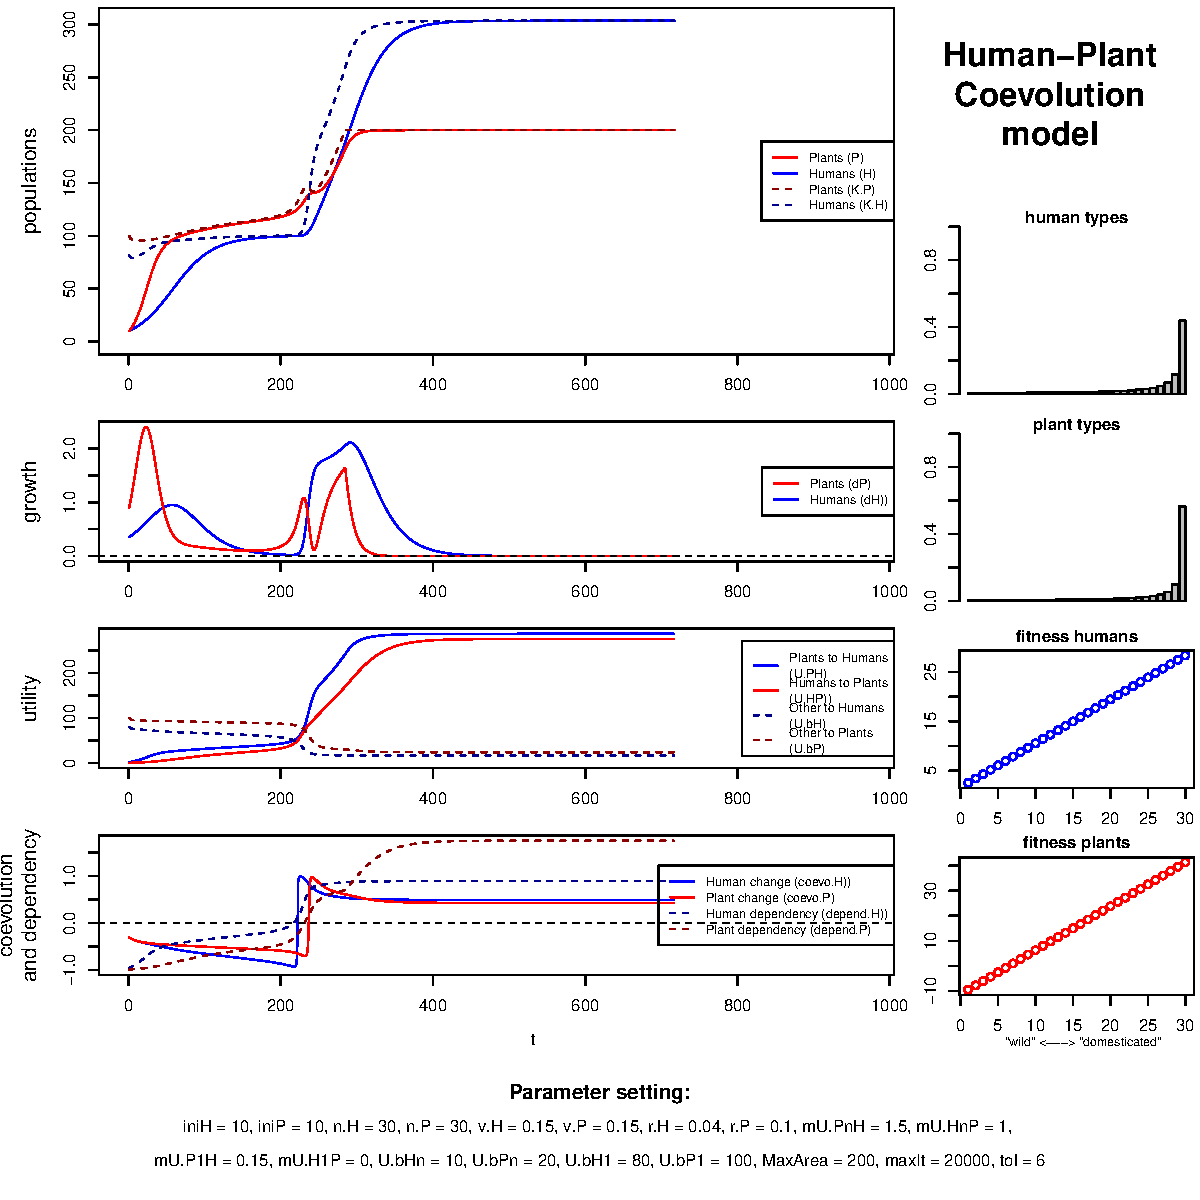
\includegraphics{hpcModel-exploration_files/figure-latex/1_run.coevo.coeta-plot-1.pdf}

\emph{Output end-state variables} at the end state:

\begin{longtable}[]{@{}ll@{}}
\toprule
Abbreviation & Value\tabularnewline
\midrule
\endhead
\texttt{time} & 716\tabularnewline
\texttt{coevo.H} & 0.6922901\tabularnewline
\texttt{coevo.P} & 0.7687119\tabularnewline
\texttt{depend.H} & 0.8913384\tabularnewline
\texttt{depend.P} & 1.7541986\tabularnewline
\texttt{timing.H} & 236\tabularnewline
\texttt{timing.P} & 252\tabularnewline
\bottomrule
\end{longtable}

Plotting population trajectories with \emph{ggplot}:

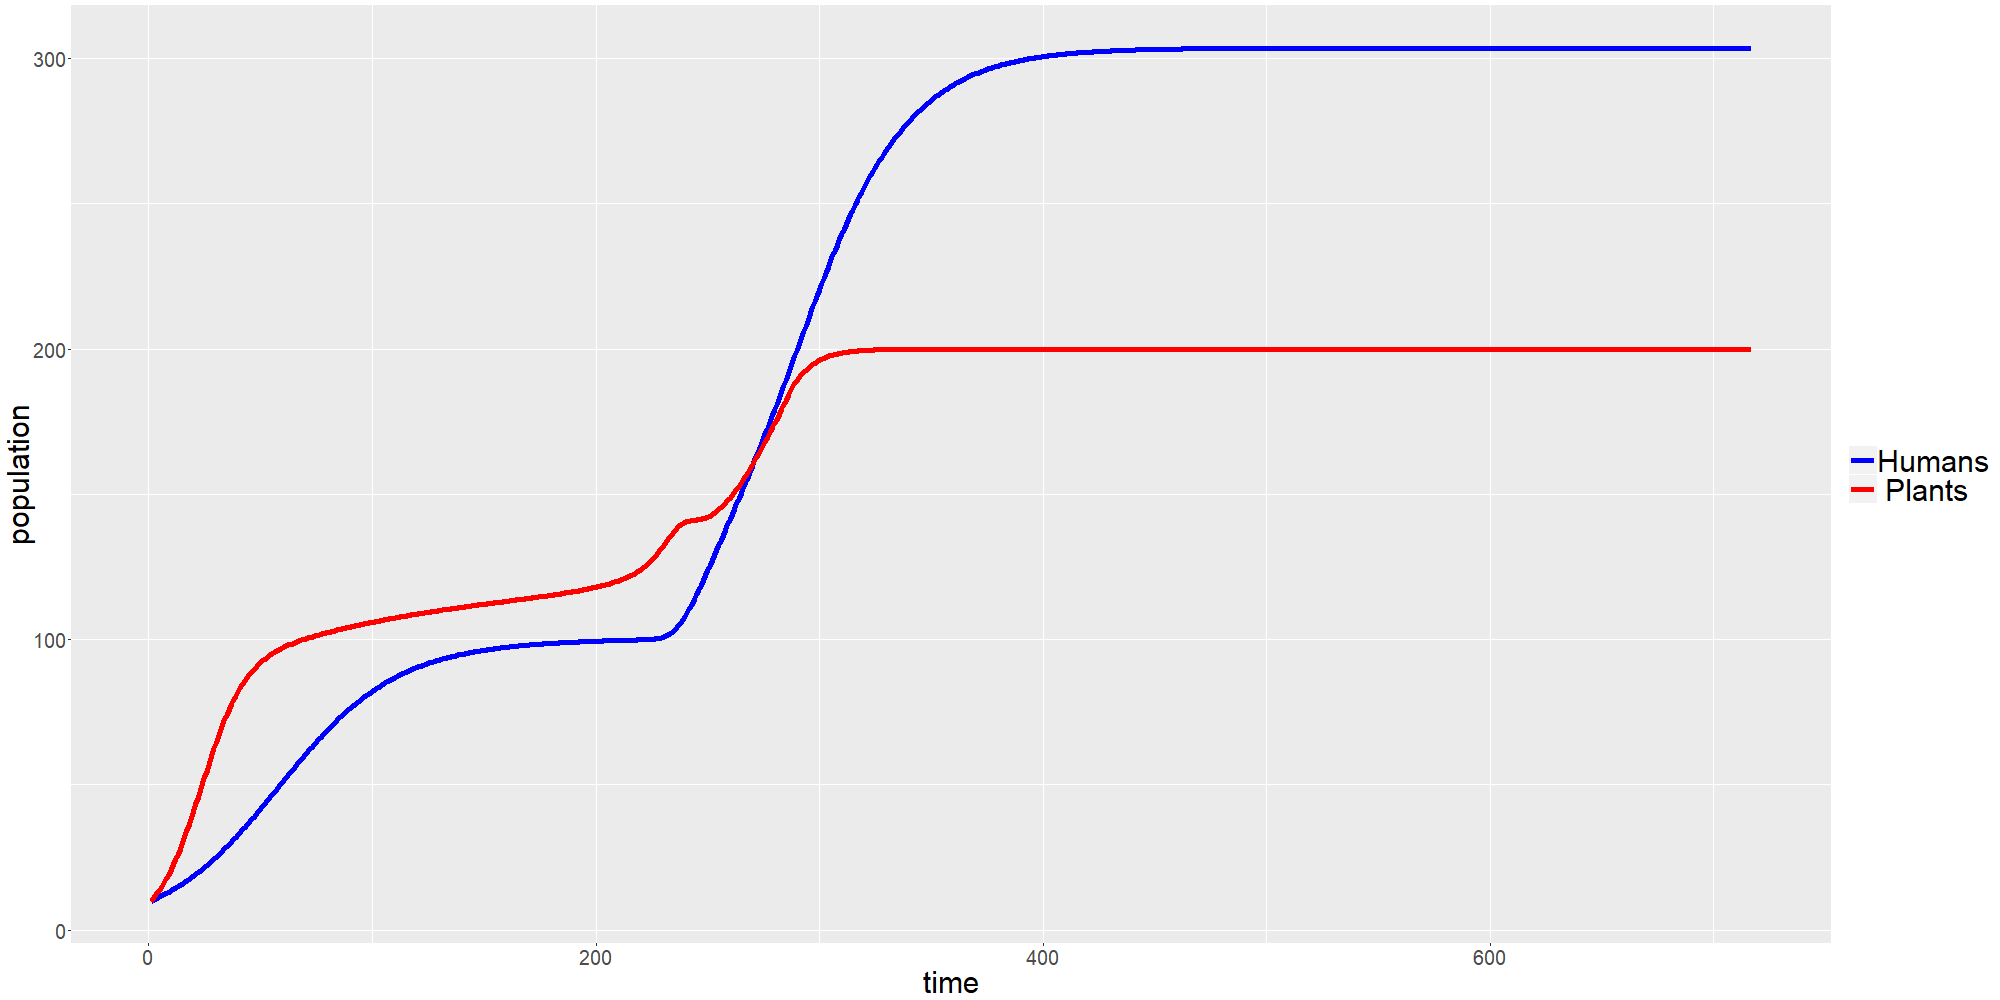
\includegraphics[width=1\linewidth]{plots/1_singleRun-ggplot-coevo.coeta}

Animated GIF showing the \emph{sequence of states} throughout the simulation:

\hypertarget{no-coevolution}{%
\section{No coevolution}\label{no-coevolution}}

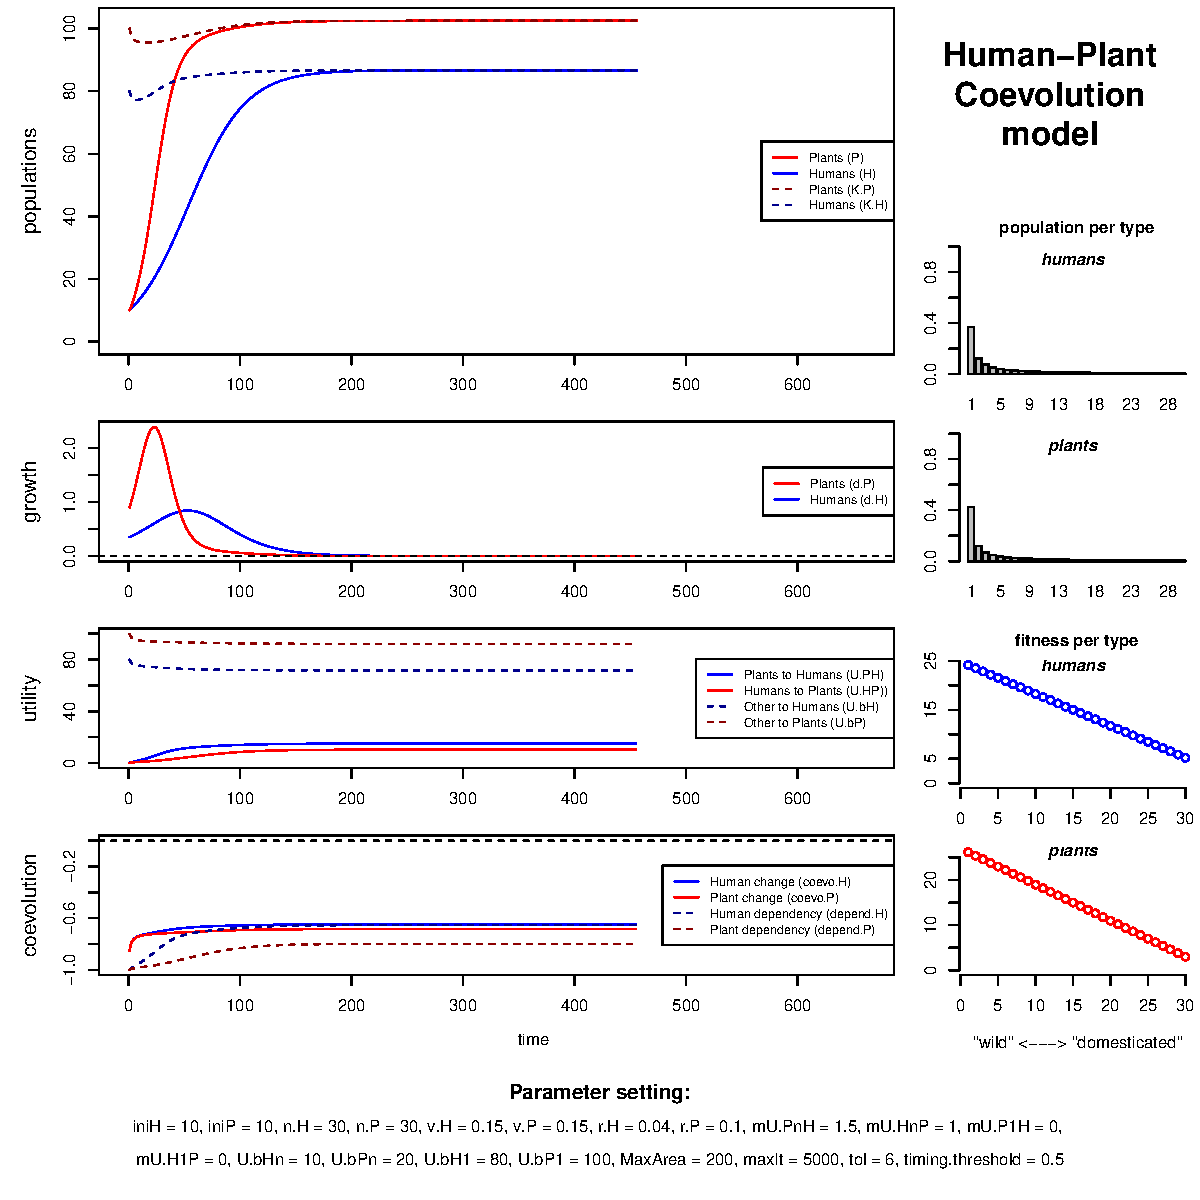
\includegraphics{hpcModel-exploration_files/figure-latex/1_run.no.coevo-plot-1.pdf}

\hypertarget{coevolution-with-early-cultivation}{%
\section{Coevolution with early cultivation}\label{coevolution-with-early-cultivation}}

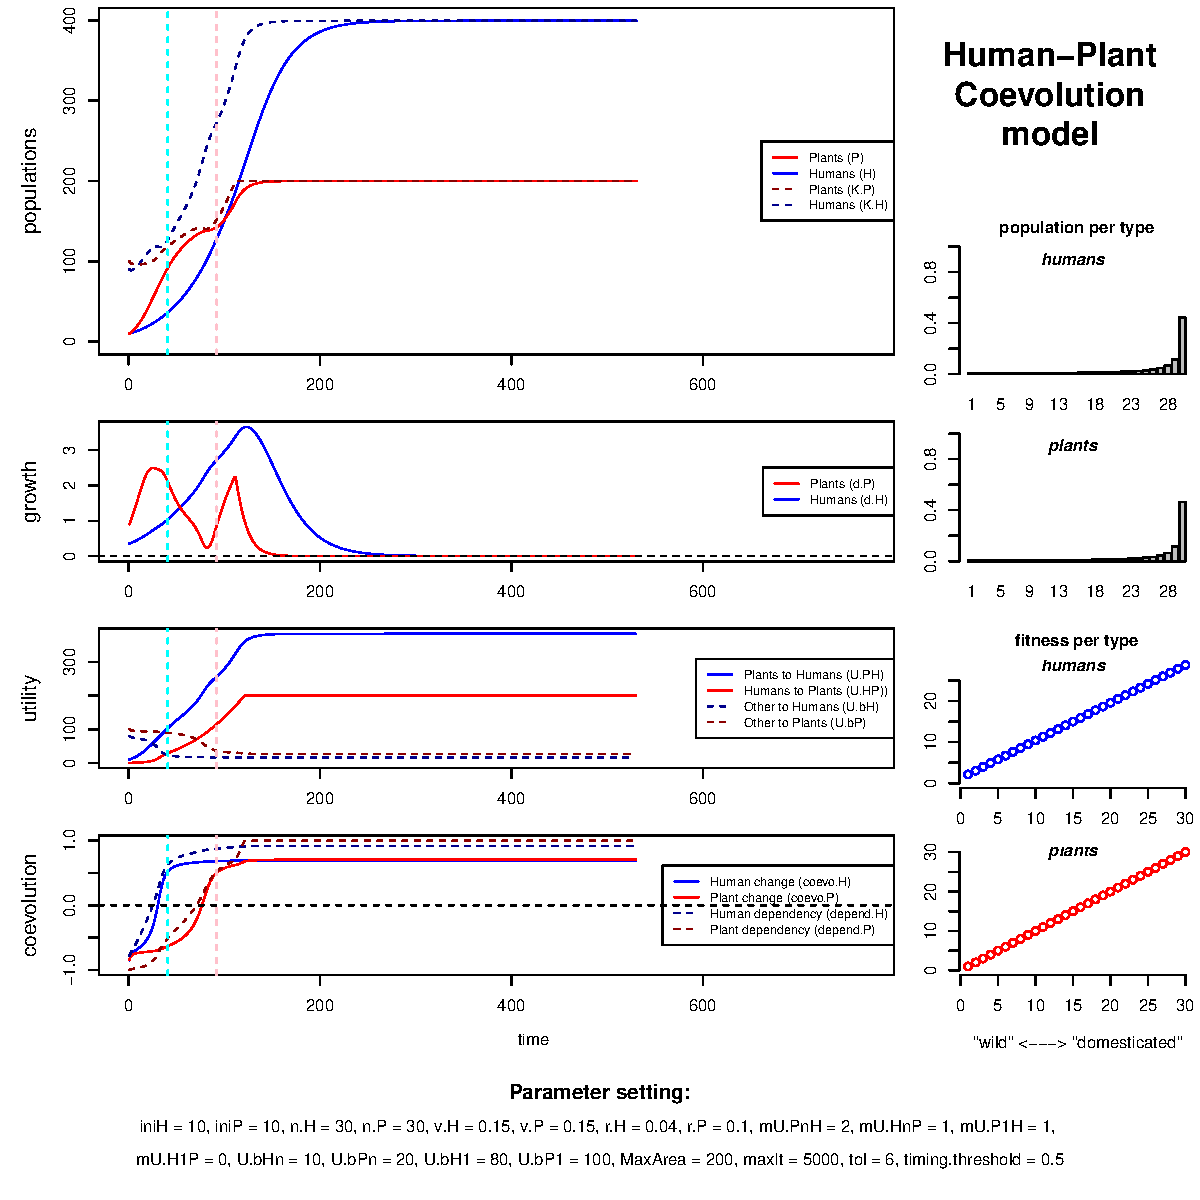
\includegraphics{hpcModel-exploration_files/figure-latex/1_run.coevo.early.cult-plot-1.pdf}

\hypertarget{coevolution-with-early-domestication}{%
\section{Coevolution with early domestication}\label{coevolution-with-early-domestication}}

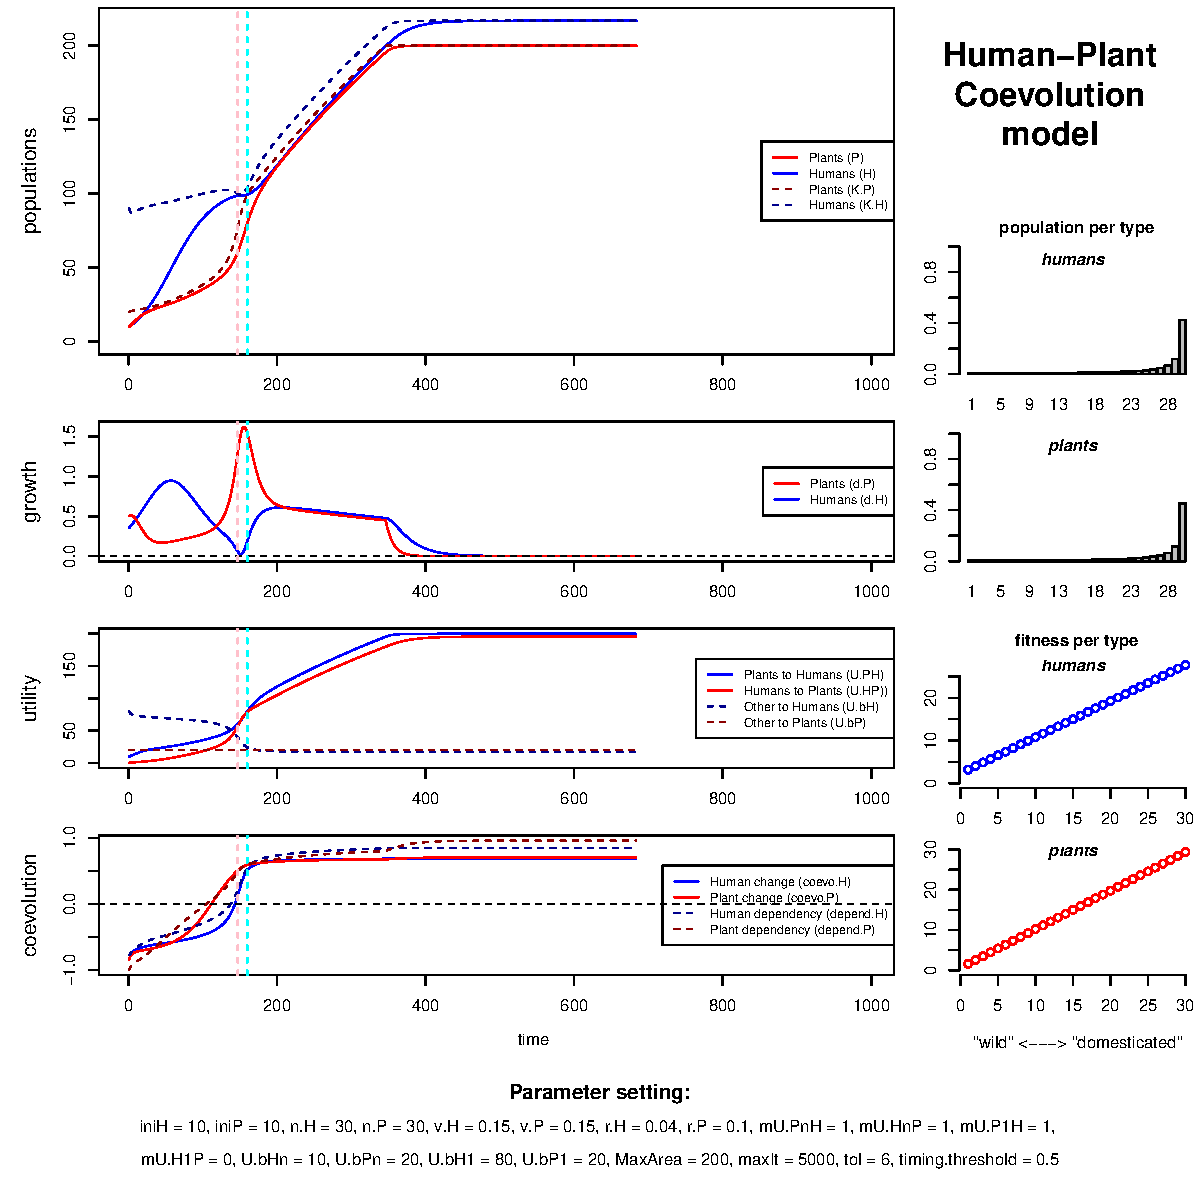
\includegraphics{hpcModel-exploration_files/figure-latex/1_run.coevo.early.dom-plot-1.pdf}

\hypertarget{cultivation-without-domestication}{%
\section{Cultivation without domestication}\label{cultivation-without-domestication}}

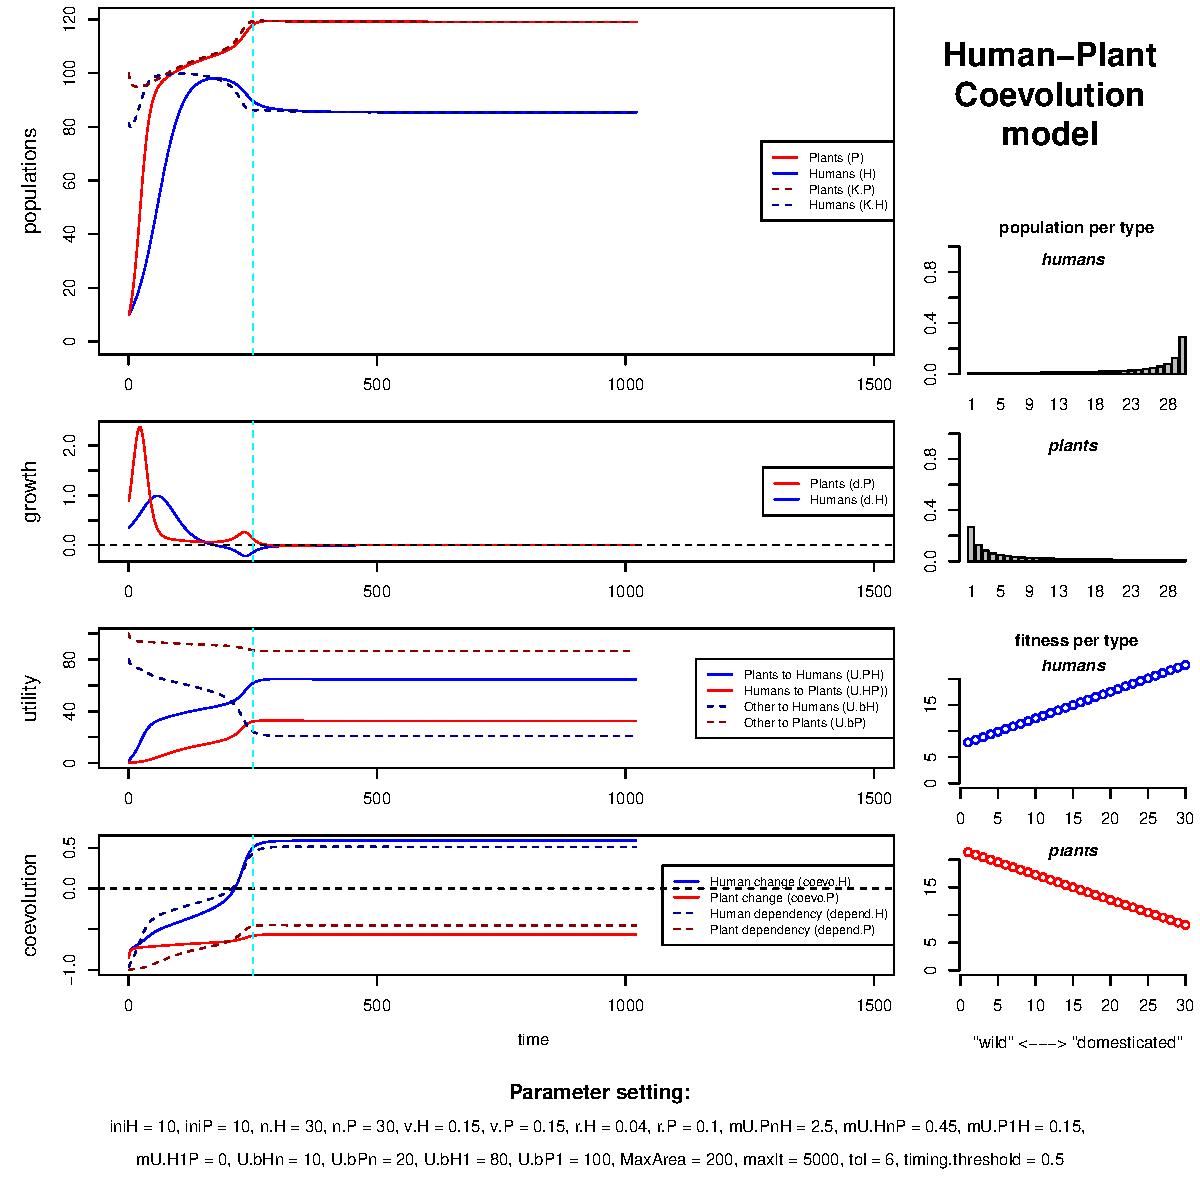
\includegraphics{hpcModel-exploration_files/figure-latex/1_run.cult.without.dom-plot-1.pdf}

\hypertarget{coevolution-with-population-bleep}{%
\section{Coevolution with population ``bleep''}\label{coevolution-with-population-bleep}}

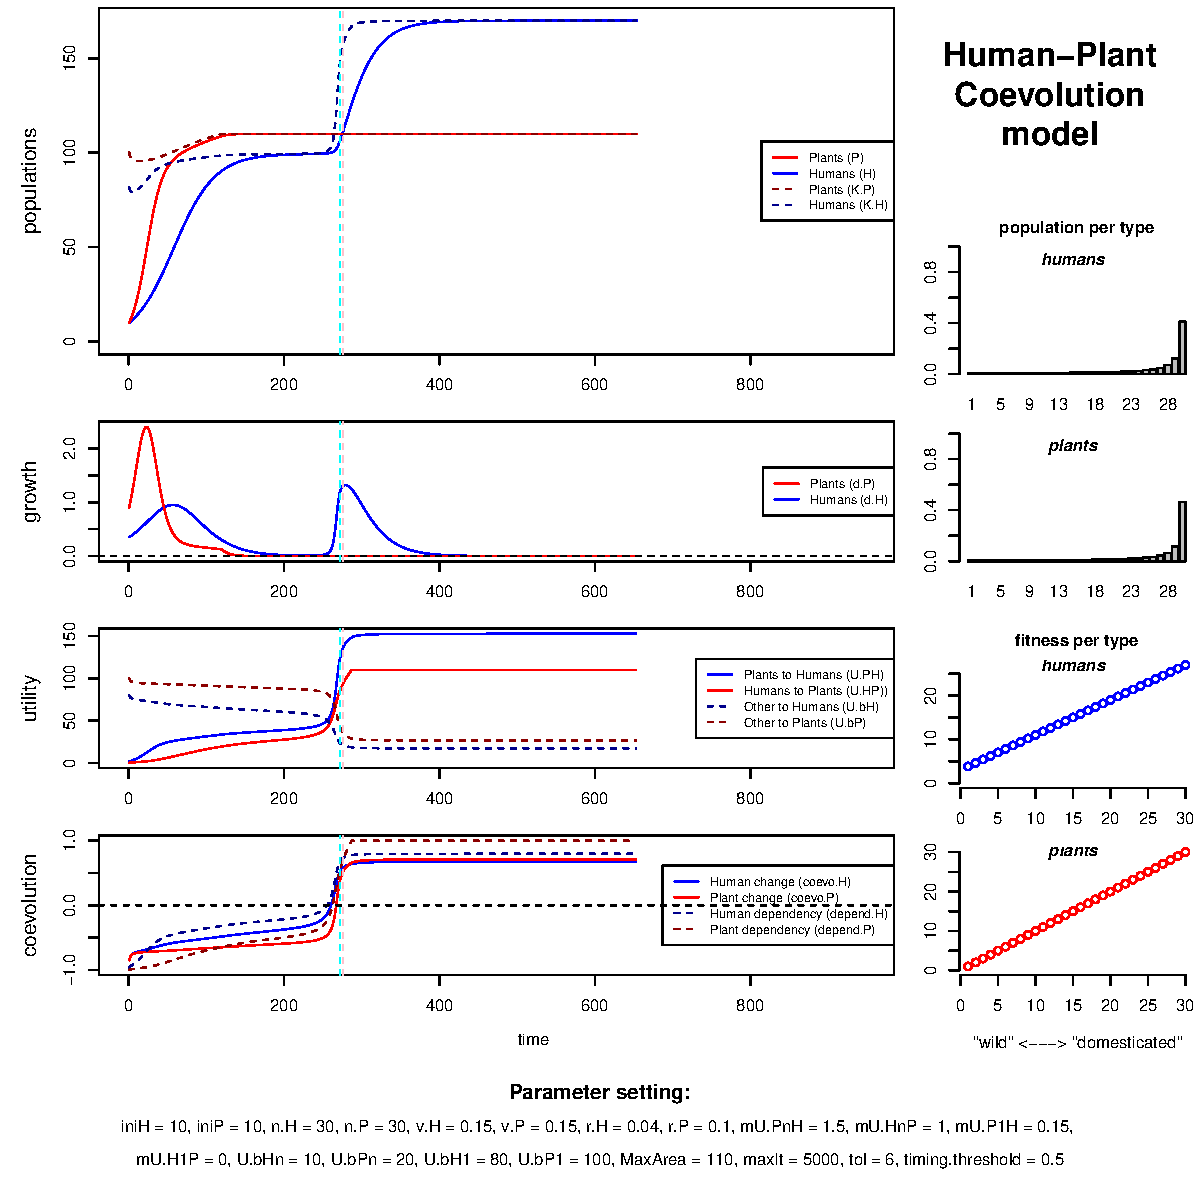
\includegraphics{hpcModel-exploration_files/figure-latex/1_run.coevo.bleep-plot-1.pdf}

\hypertarget{coevolution-with-population-boom}{%
\section{Coevolution with population ``boom''}\label{coevolution-with-population-boom}}

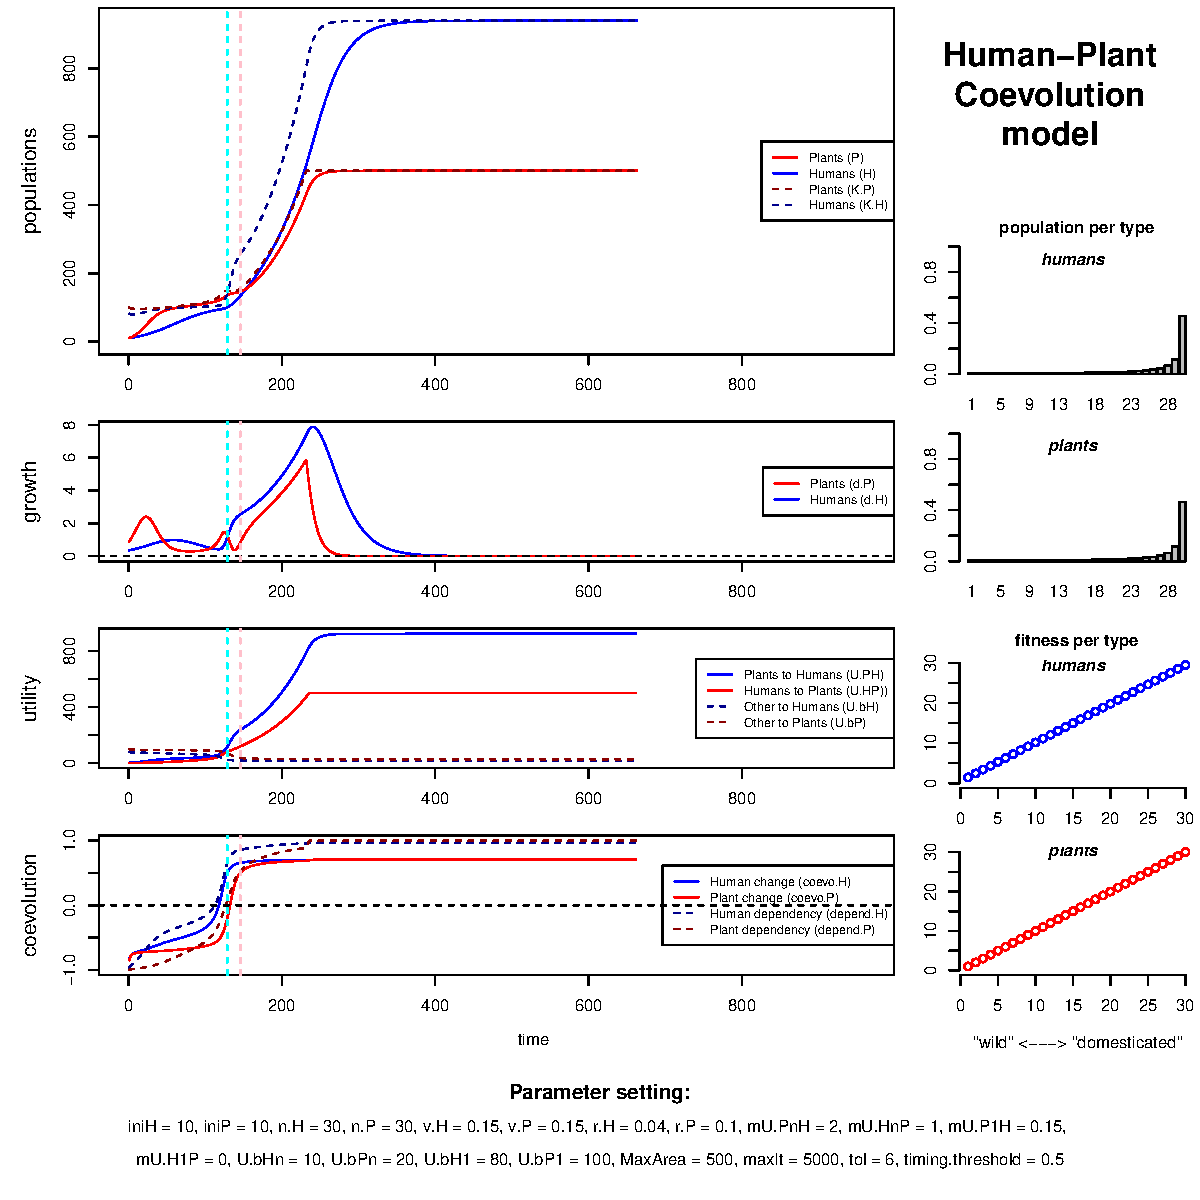
\includegraphics{hpcModel-exploration_files/figure-latex/1_run.coevo.boom-plot-1.pdf}

\hypertarget{coevolution-with-long-population-boom}{%
\section{Coevolution with long population ``boom''}\label{coevolution-with-long-population-boom}}

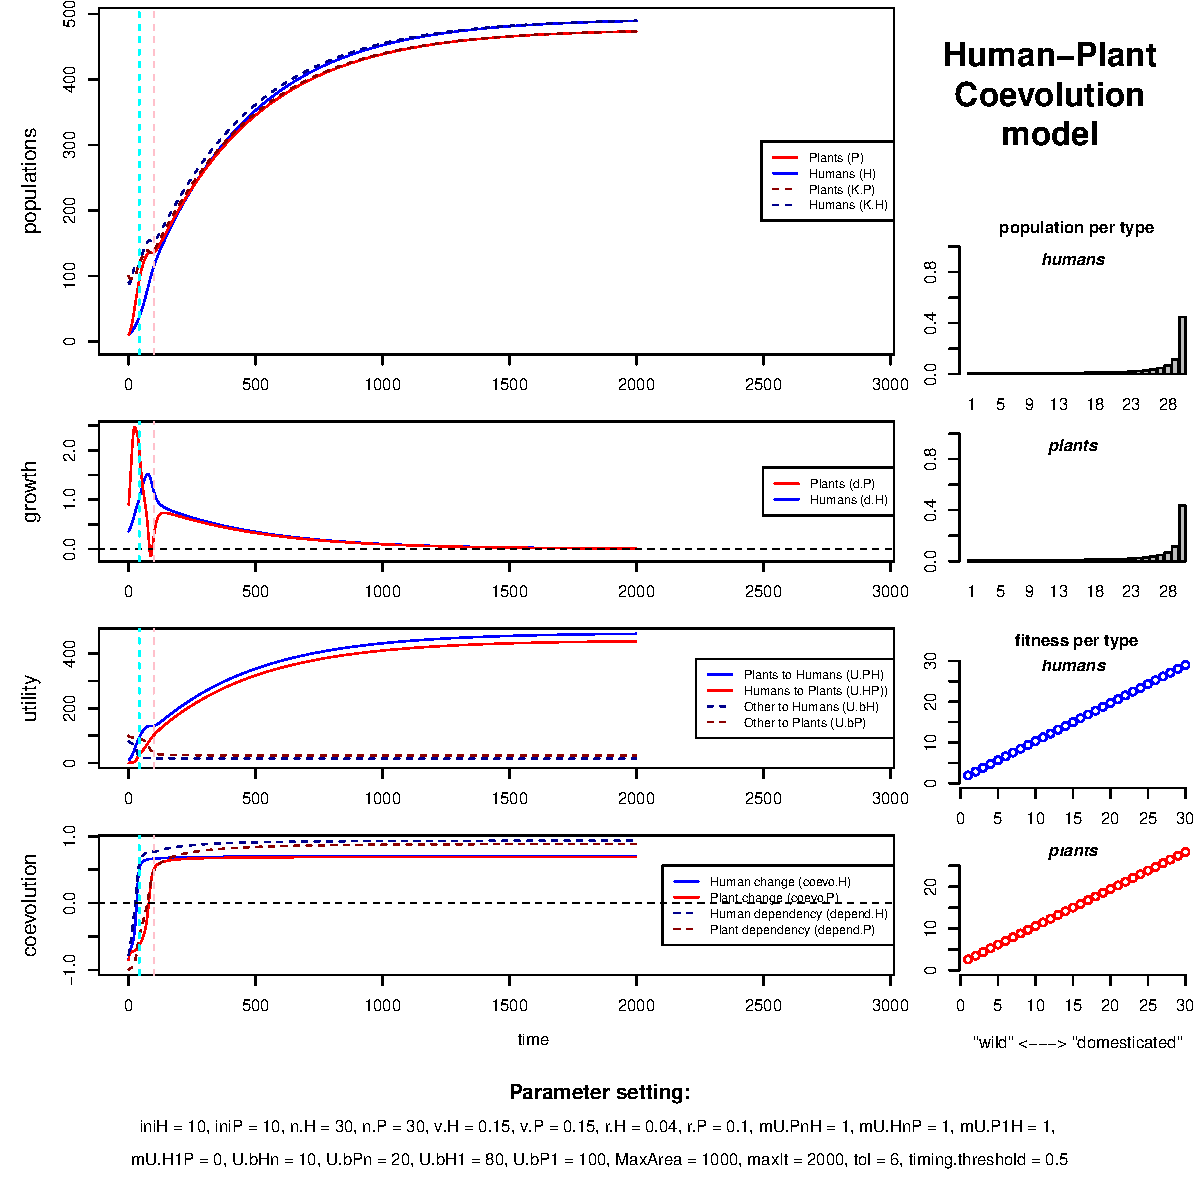
\includegraphics{hpcModel-exploration_files/figure-latex/1_run.coevo.long.boom-plot-1.pdf}

\hypertarget{semi-coevolution-stationary-point}{%
\section{Semi-coevolution (stationary point)}\label{semi-coevolution-stationary-point}}

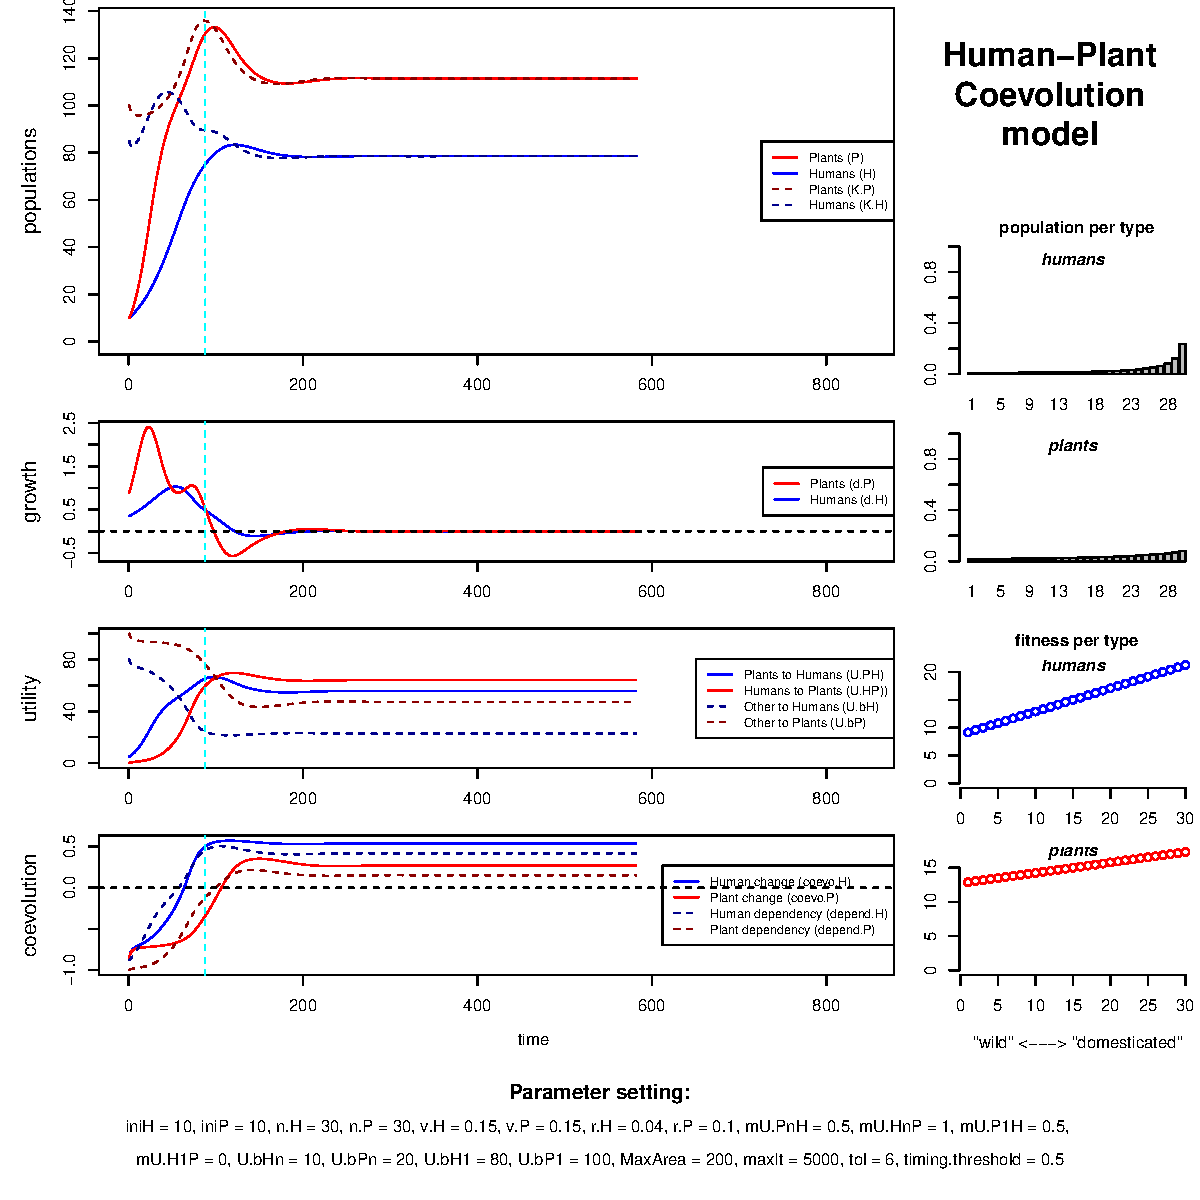
\includegraphics{hpcModel-exploration_files/figure-latex/1_run.semicoevo-plot-1.pdf}

\hypertarget{semi-coevolution-oscillations}{%
\section{Semi-coevolution (oscillations)}\label{semi-coevolution-oscillations}}

\emph{Parameter setting}:

\begin{tabular}{l|l}
\hline
parameter & values\\
\hline
iniH & 10\\
\hline
iniP & 10\\
\hline
n.H & 30\\
\hline
n.P & 30\\
\hline
v.H & 0.15\\
\hline
v.P & 0.15\\
\hline
r.H & 0.04\\
\hline
r.P & 0.1\\
\hline
mU.PnH & 0.5\\
\hline
mU.HnP & 0.9\\
\hline
mU.P1H & 0.5\\
\hline
mU.H1P & 0\\
\hline
U.bHn & 20\\
\hline
U.bPn & 20\\
\hline
U.bH1 & 100\\
\hline
U.bP1 & 100\\
\hline
MaxArea & 200\\
\hline
maxIt & 2000\\
\hline
tol & 6\\
\hline
timing.threshold & 0.5\\
\hline
\end{tabular}

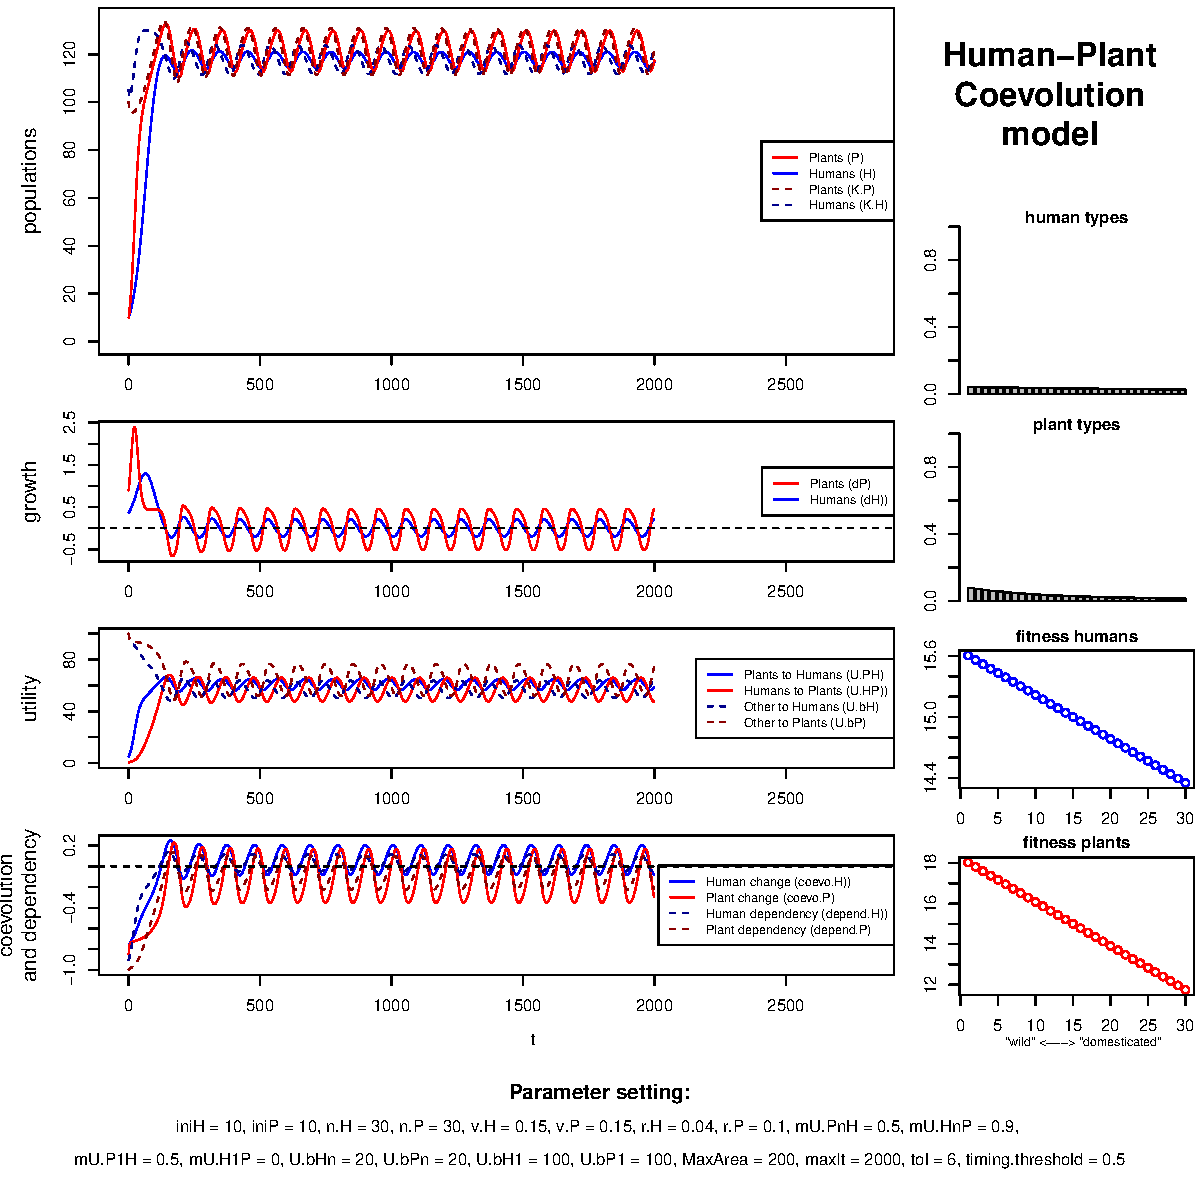
\includegraphics{hpcModel-exploration_files/figure-latex/1_run.semicoevo.osc-plot-1.pdf}

\hypertarget{one-parameter-exploration}{%
\chapter{One parameter exploration}\label{one-parameter-exploration}}

\hypertarget{full-example-tableplot-alternatives}{%
\section{Full example (table+plot alternatives)}\label{full-example-tableplot-alternatives}}

\hypertarget{utility-per-capita-of-type-n-plants-to-humans-baru_p_nh}{%
\subsection{\texorpdfstring{utility per capita \textbf{of} type n plants \textbf{to} humans (\(\bar{U}_{P_{n}H}\)):}{utility per capita of type n plants to humans (\textbackslash{}bar\{U\}\_\{P\_\{n\}H\}):}}\label{utility-per-capita-of-type-n-plants-to-humans-baru_p_nh}}

\begin{tabular}{l|l}
\hline
parameter & value\\
\hline
iniH & 10\\
\hline
iniP & 10\\
\hline
n.H & 30\\
\hline
n.P & 30\\
\hline
v.H & 0.15\\
\hline
v.P & 0.15\\
\hline
r.H & 0.04\\
\hline
r.P & 0.1\\
\hline
mU.PnH & 0.5 - 2.5 (sample = 100 )\\
\hline
mU.HnP & 1\\
\hline
mU.P1H & 0.15\\
\hline
mU.H1P & 0\\
\hline
U.bHn & 10\\
\hline
U.bPn & 20\\
\hline
U.bH1 & 80\\
\hline
U.bP1 & 100\\
\hline
MaxArea & 200\\
\hline
\end{tabular}

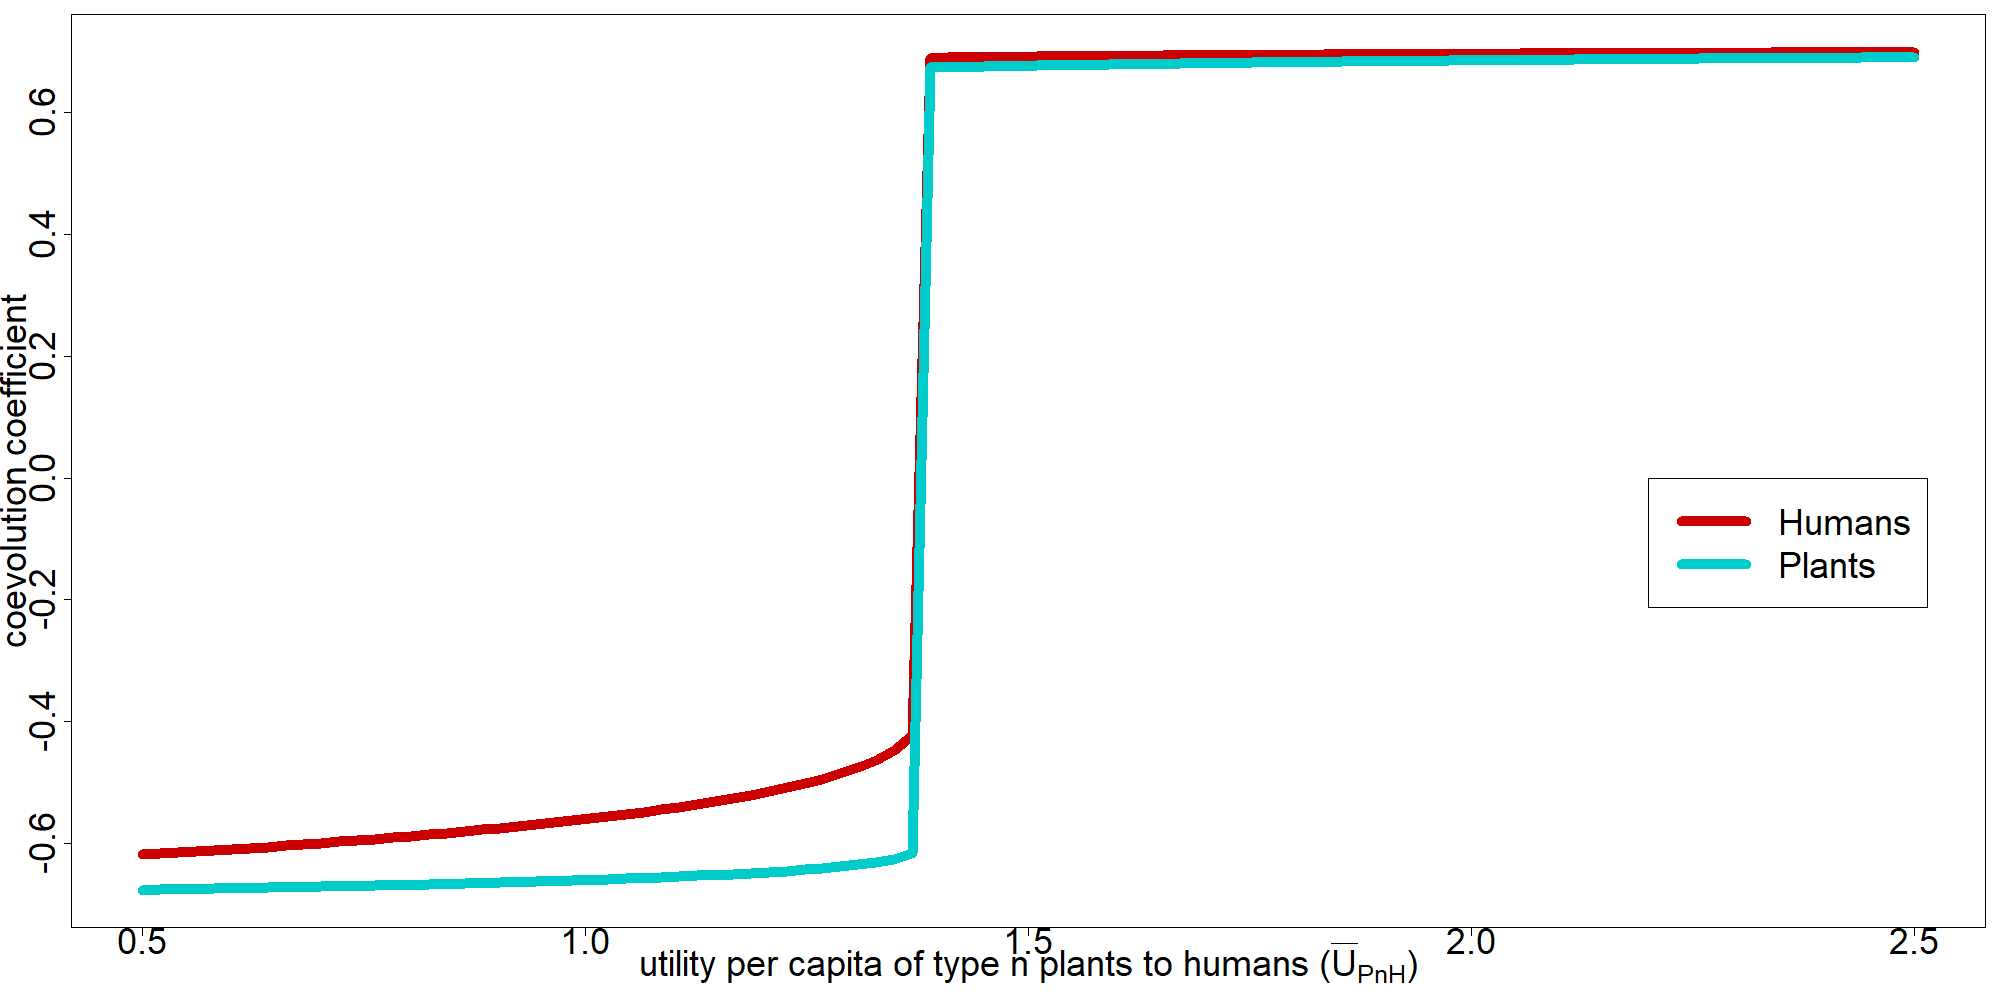
\includegraphics[width=1\linewidth]{plots/2_onePar-mU.PnH_ggbifplot}

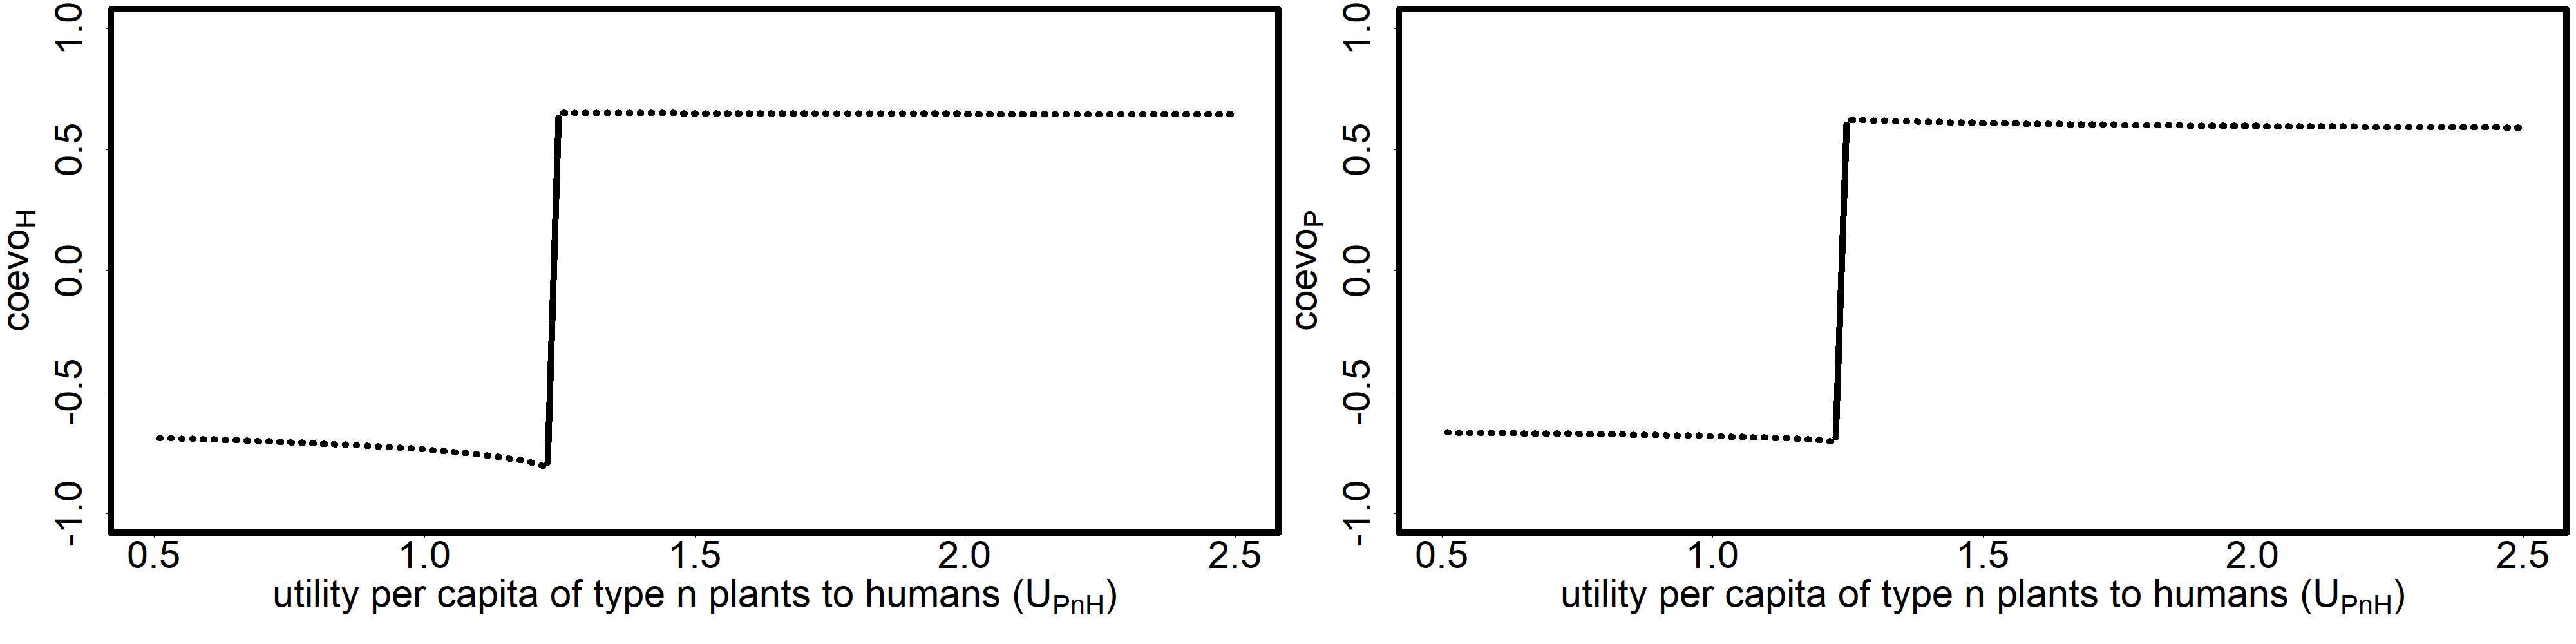
\includegraphics[width=1\linewidth]{plots/2_onePar-mU.PnH_bifplot-pair}

\begin{center}\rule{0.5\linewidth}{\linethickness}\end{center}

\hypertarget{exploration-on-default-setting-for-each-parameter}{%
\section{Exploration on `default' setting for each parameter:}\label{exploration-on-default-setting-for-each-parameter}}

\hypertarget{initial-populations-of-humans-and-plants-init_hinit_p}{%
\subsection{\texorpdfstring{Initial populations of humans and plants (\(init_{H},\,init_{P}\)):}{Initial populations of humans and plants (init\_\{H\},\textbackslash{},init\_\{P\}):}}\label{initial-populations-of-humans-and-plants-init_hinit_p}}

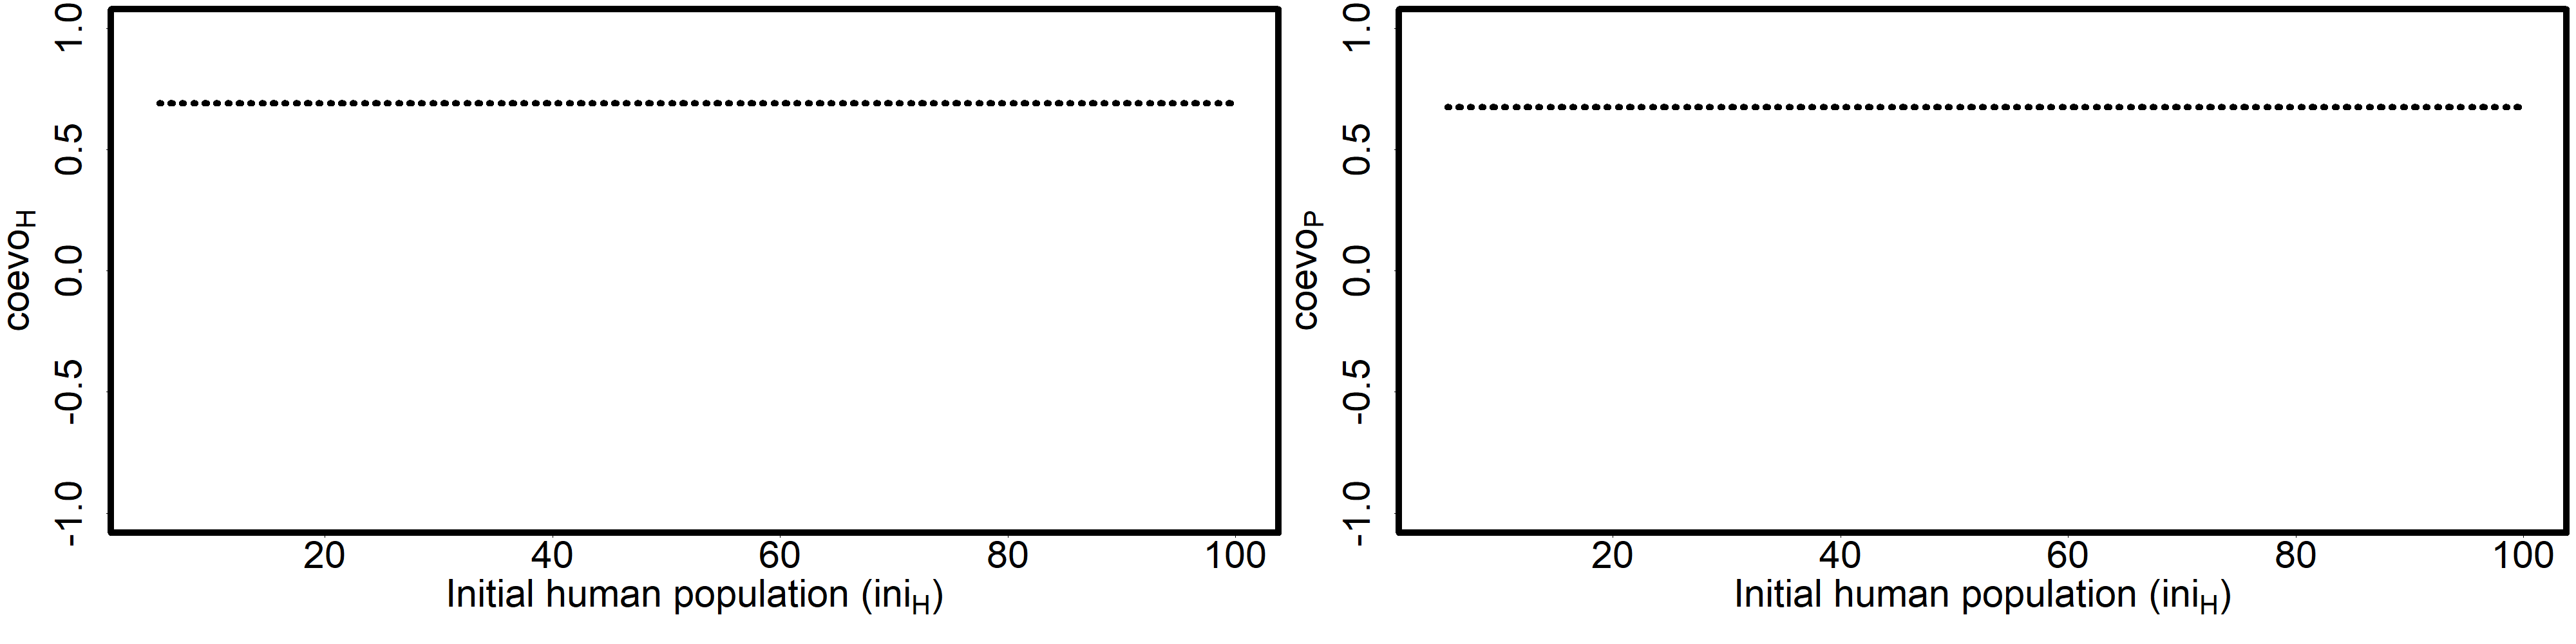
\includegraphics[width=1\linewidth]{plots/2_onePar-init.H_bifplot-pair}

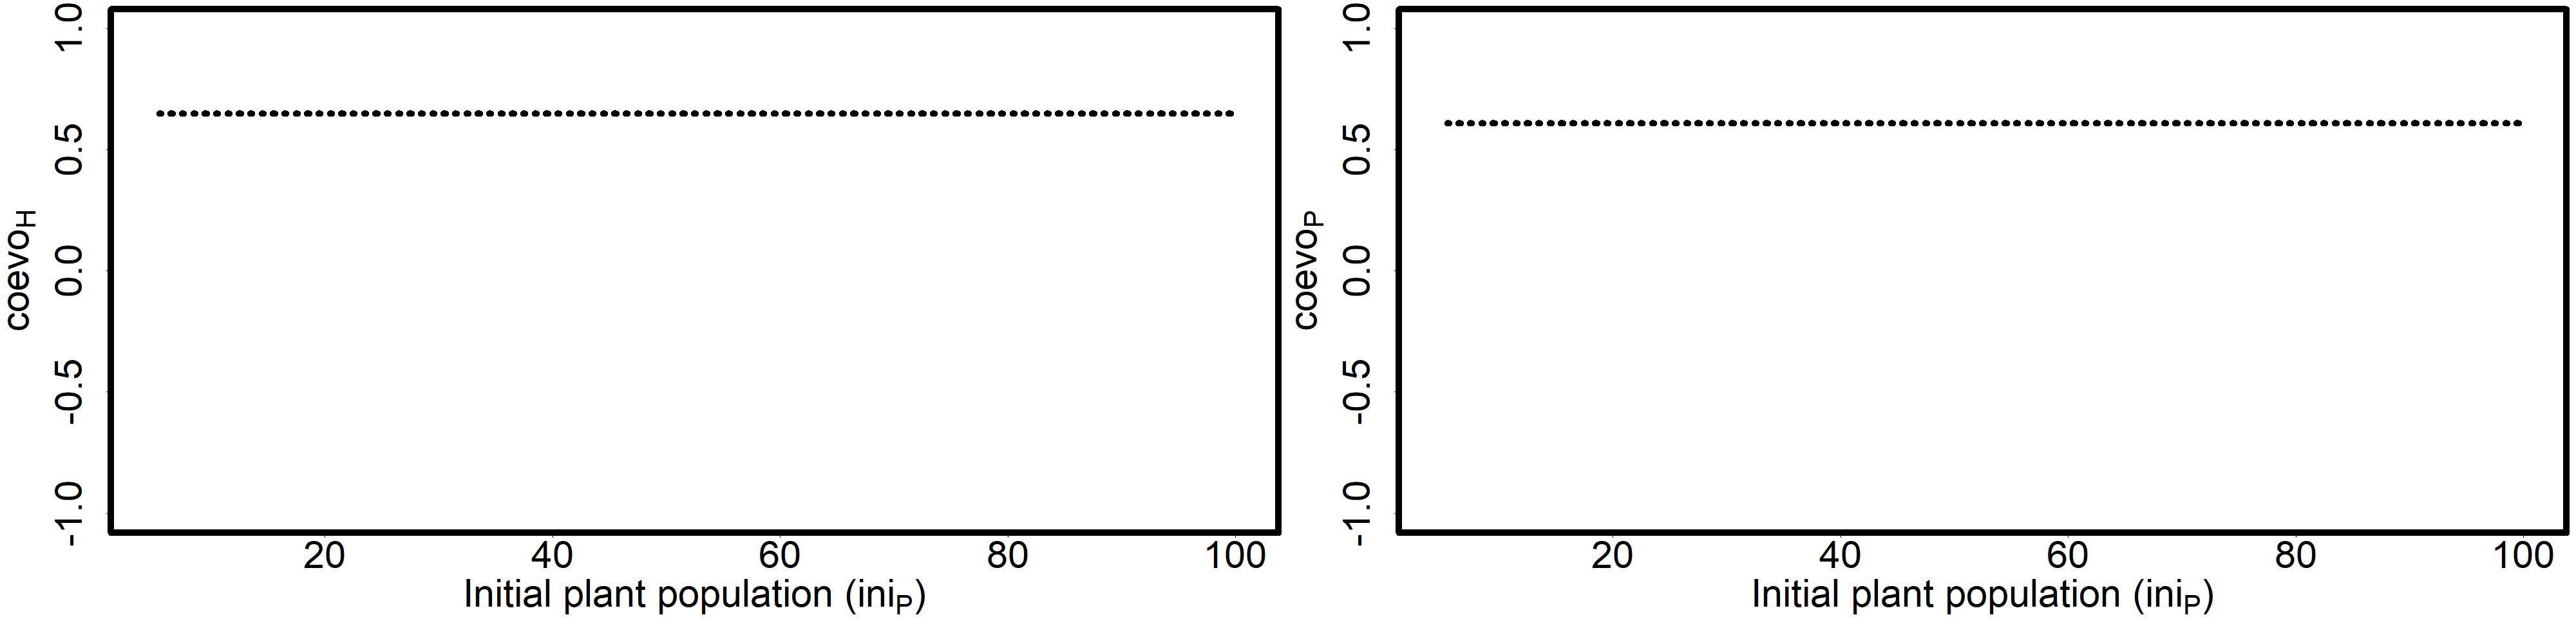
\includegraphics[width=1\linewidth]{plots/2_onePar-init.P_bifplot-pair}

\hypertarget{number-of-types-of-humans-and-plants-n_hn_p}{%
\subsection{\texorpdfstring{Number of types of humans and plants (\(n_{H},\,n_{P}\)):}{Number of types of humans and plants (n\_\{H\},\textbackslash{},n\_\{P\}):}}\label{number-of-types-of-humans-and-plants-n_hn_p}}

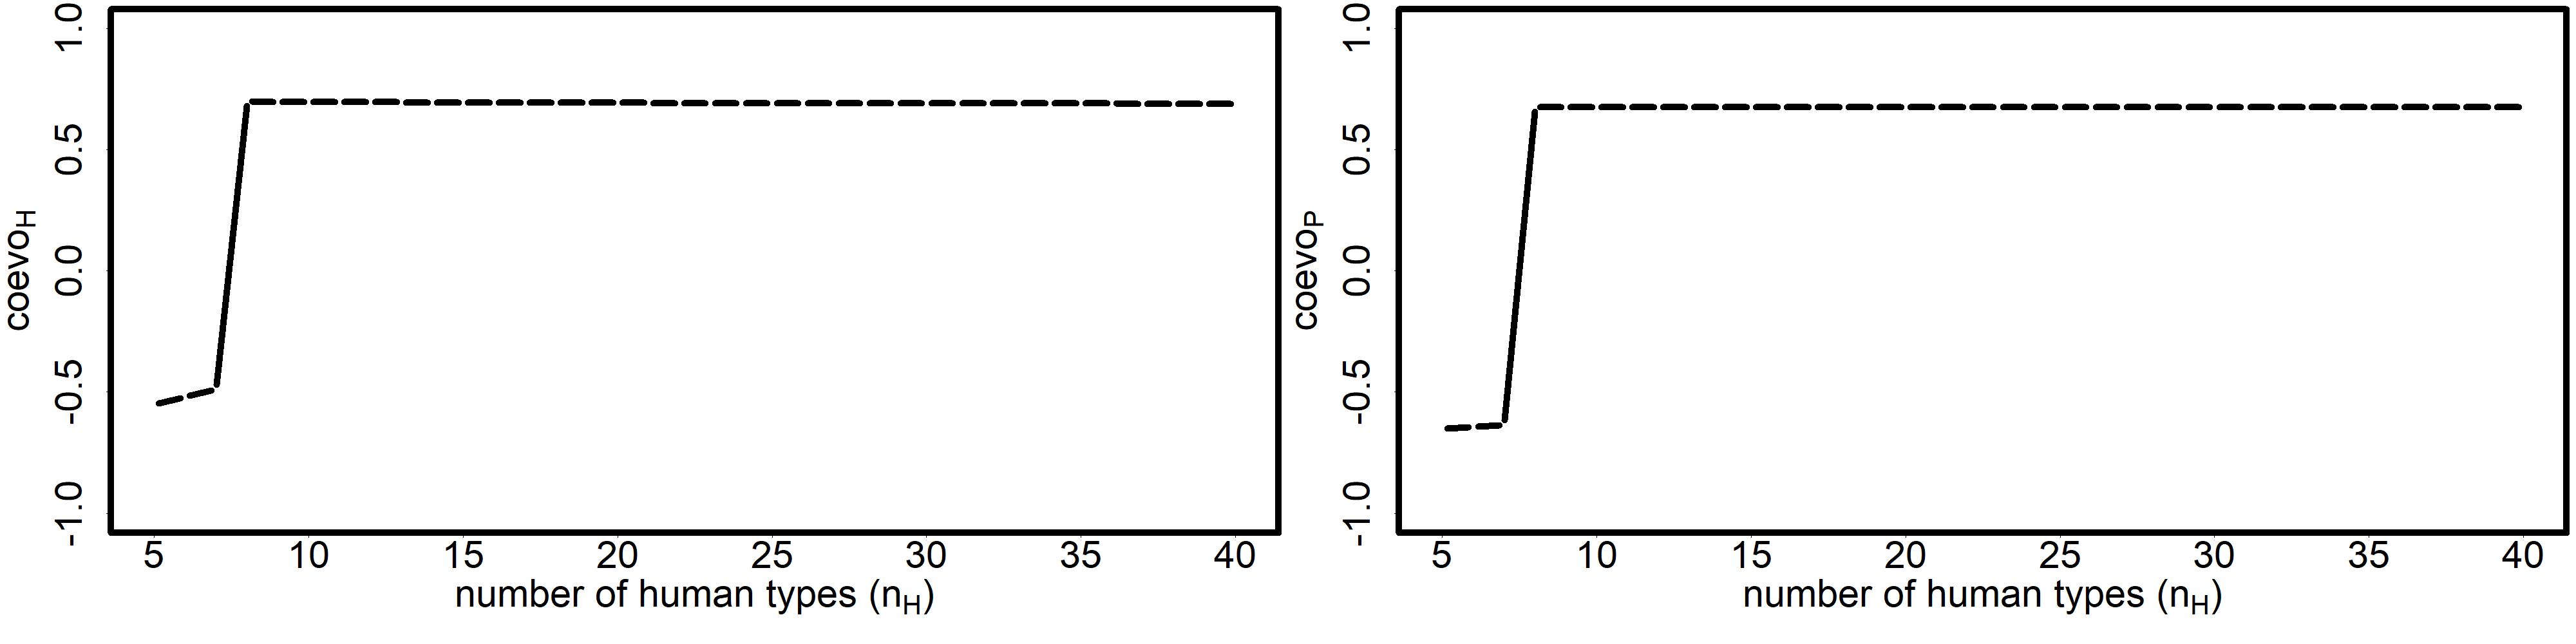
\includegraphics[width=1\linewidth]{plots/2_onePar-n.H_bifplot-pair}

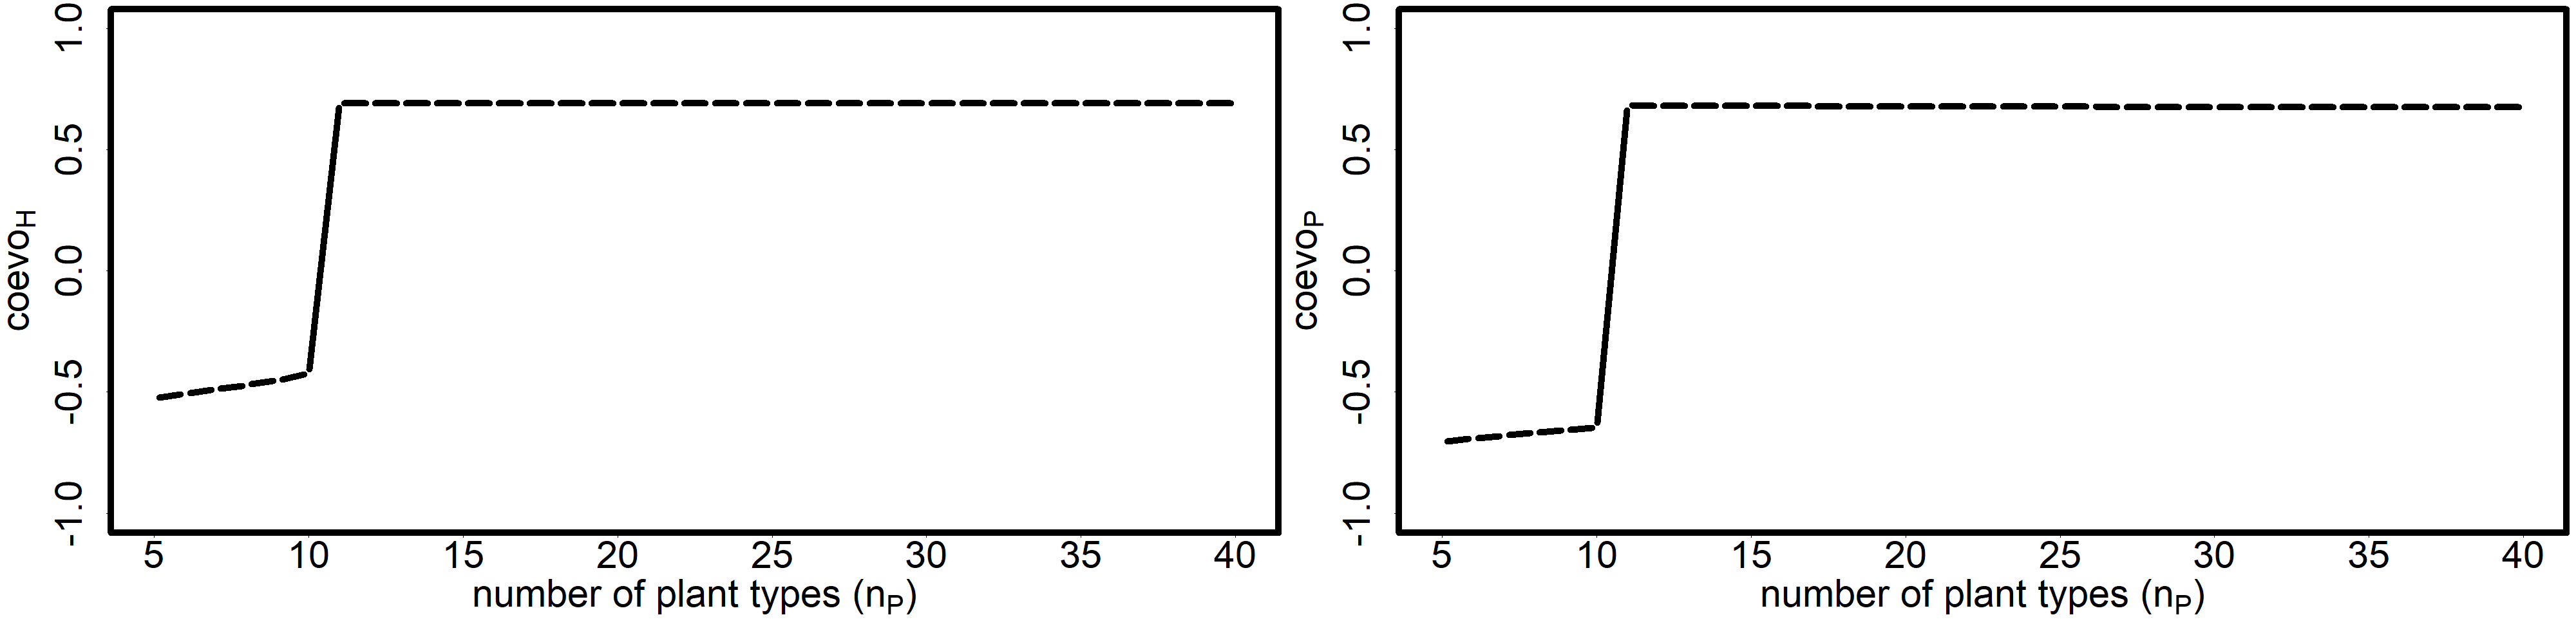
\includegraphics[width=1\linewidth]{plots/2_onePar-n.P_bifplot-pair}

\hypertarget{level-of-undirected-variation-in-humans-and-plants-v_hv_p}{%
\subsection{\texorpdfstring{level of undirected variation in humans and plants (\(v_{H},\,v_{P}\)):}{level of undirected variation in humans and plants (v\_\{H\},\textbackslash{},v\_\{P\}):}}\label{level-of-undirected-variation-in-humans-and-plants-v_hv_p}}

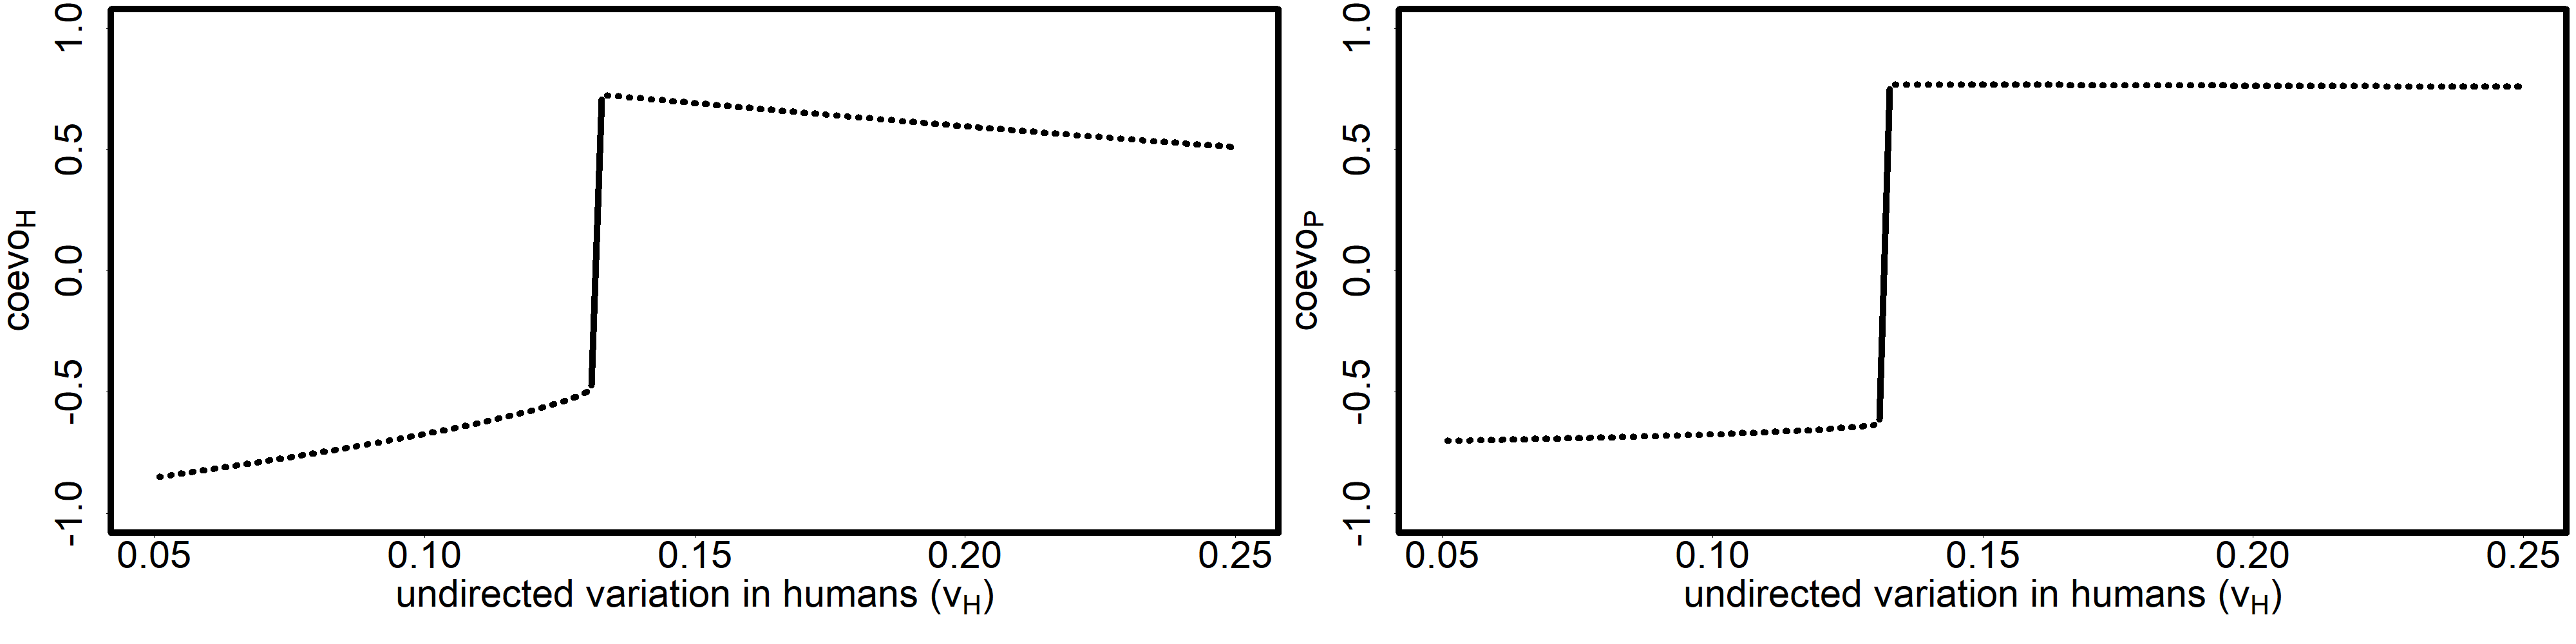
\includegraphics[width=1\linewidth]{plots/2_onePar-v.H_bifplot-pair}

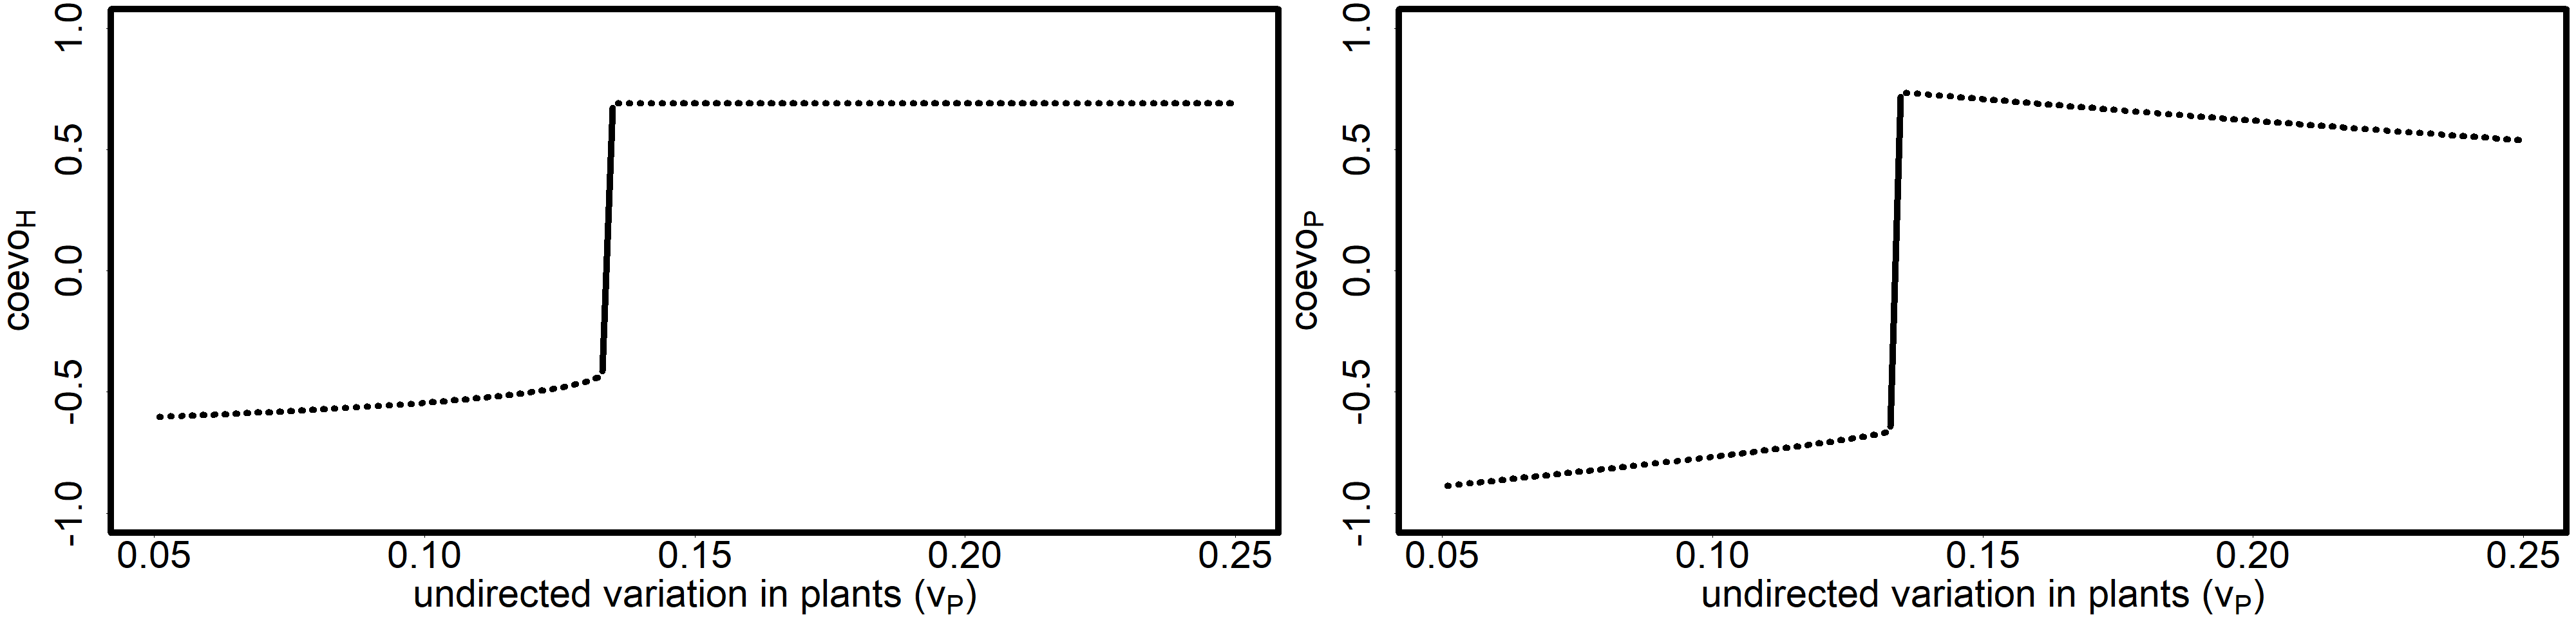
\includegraphics[width=1\linewidth]{plots/2_onePar-v.P_bifplot-pair}

\hypertarget{intrinsic-growth-rates-for-human-and-plant-populations-r_hr_p}{%
\subsection{\texorpdfstring{intrinsic growth rates for human and plant populations (\(r_{H},\,r_{P}\)):}{intrinsic growth rates for human and plant populations (r\_\{H\},\textbackslash{},r\_\{P\}):}}\label{intrinsic-growth-rates-for-human-and-plant-populations-r_hr_p}}

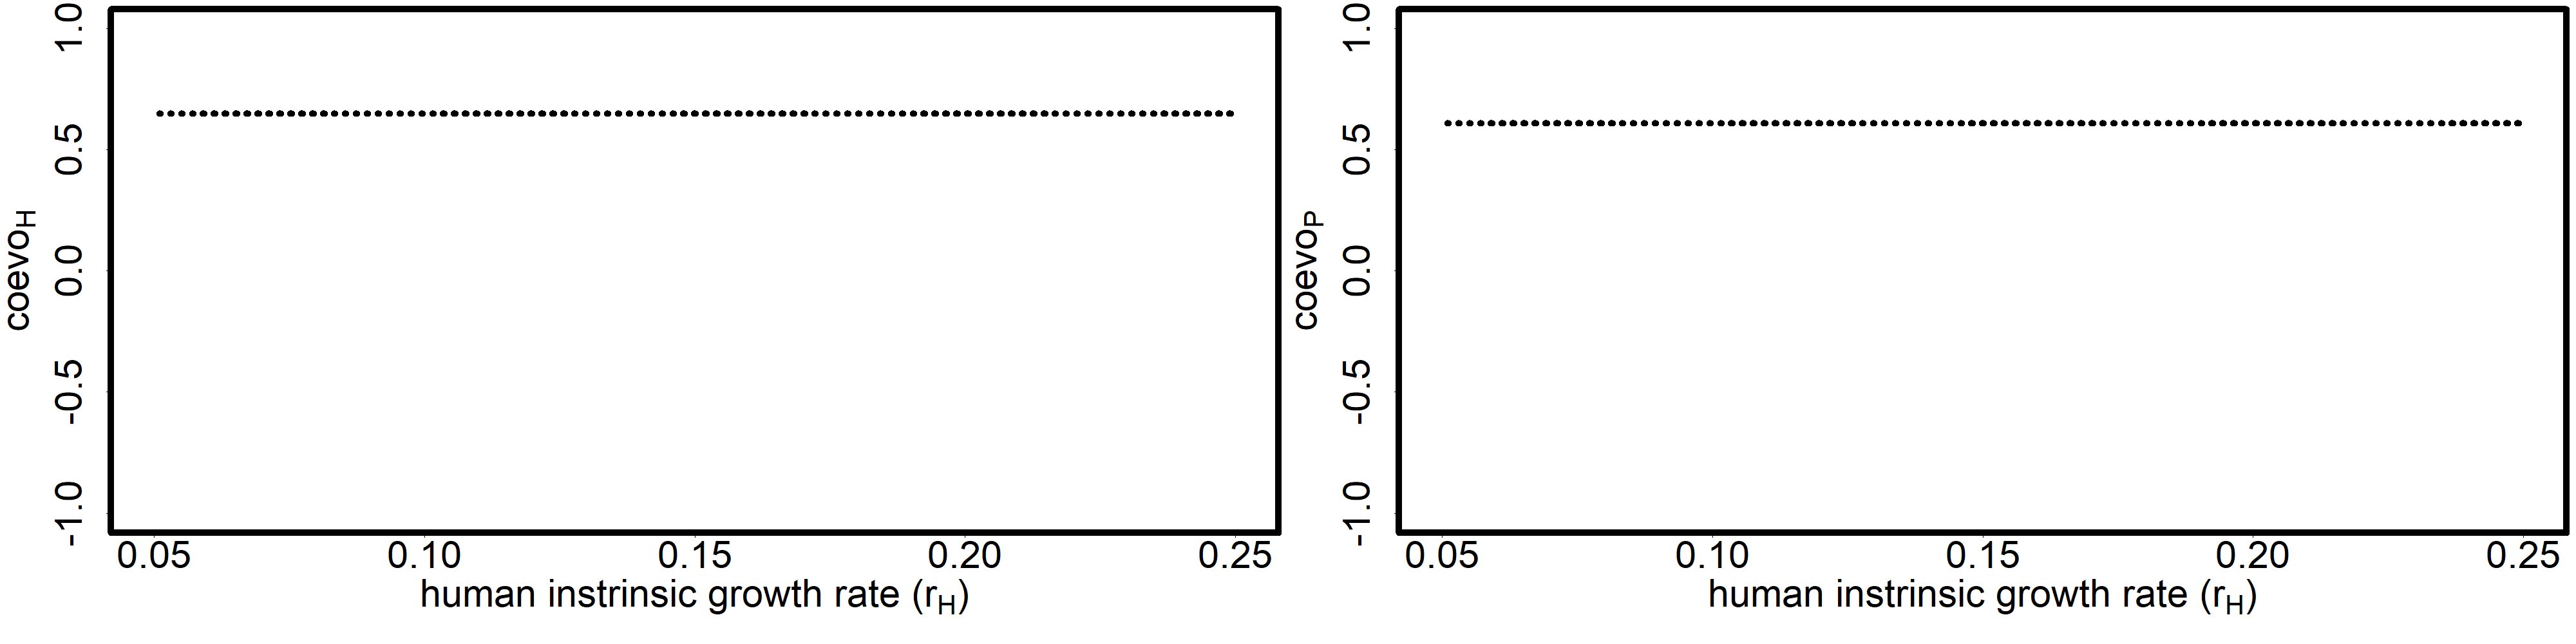
\includegraphics[width=1\linewidth]{plots/2_onePar-r.H_bifplot-pair}

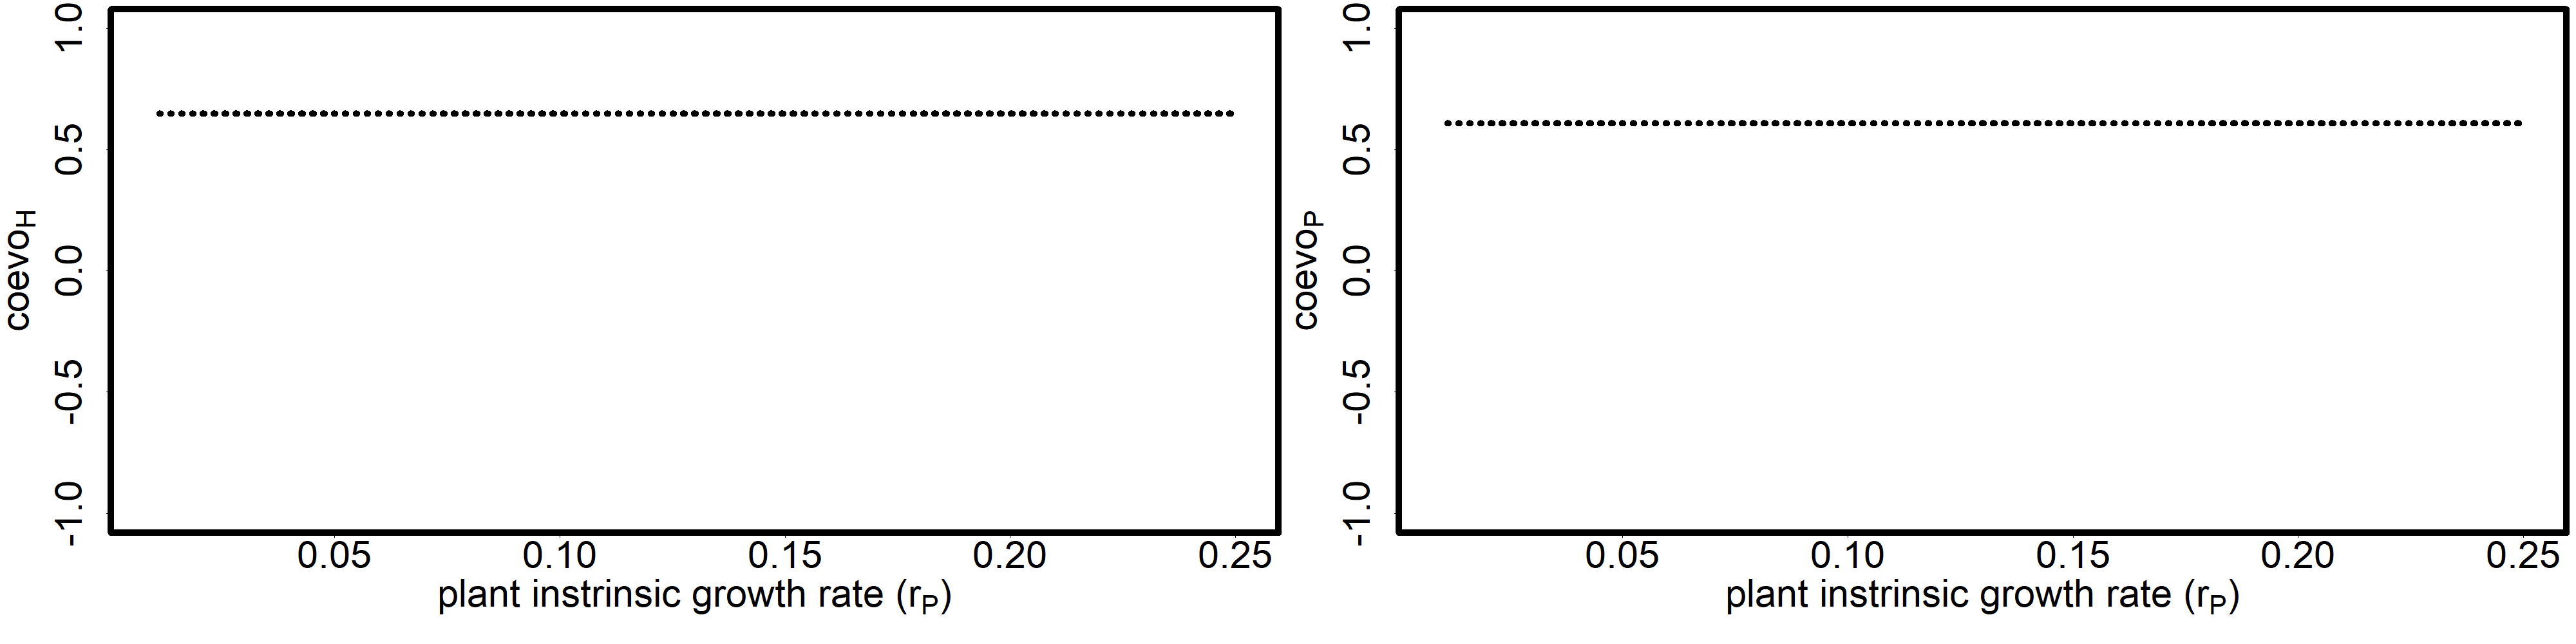
\includegraphics[width=1\linewidth]{plots/2_onePar-r.P_bifplot-pair}

\hypertarget{utility-per-capita-of-type-n-plants-to-humans-baru_p_nh-1}{%
\subsection{\texorpdfstring{utility per capita \textbf{of} type n plants \textbf{to} humans (\(\bar{U}_{P_{n}H}\)):}{utility per capita of type n plants to humans (\textbackslash{}bar\{U\}\_\{P\_\{n\}H\}):}}\label{utility-per-capita-of-type-n-plants-to-humans-baru_p_nh-1}}

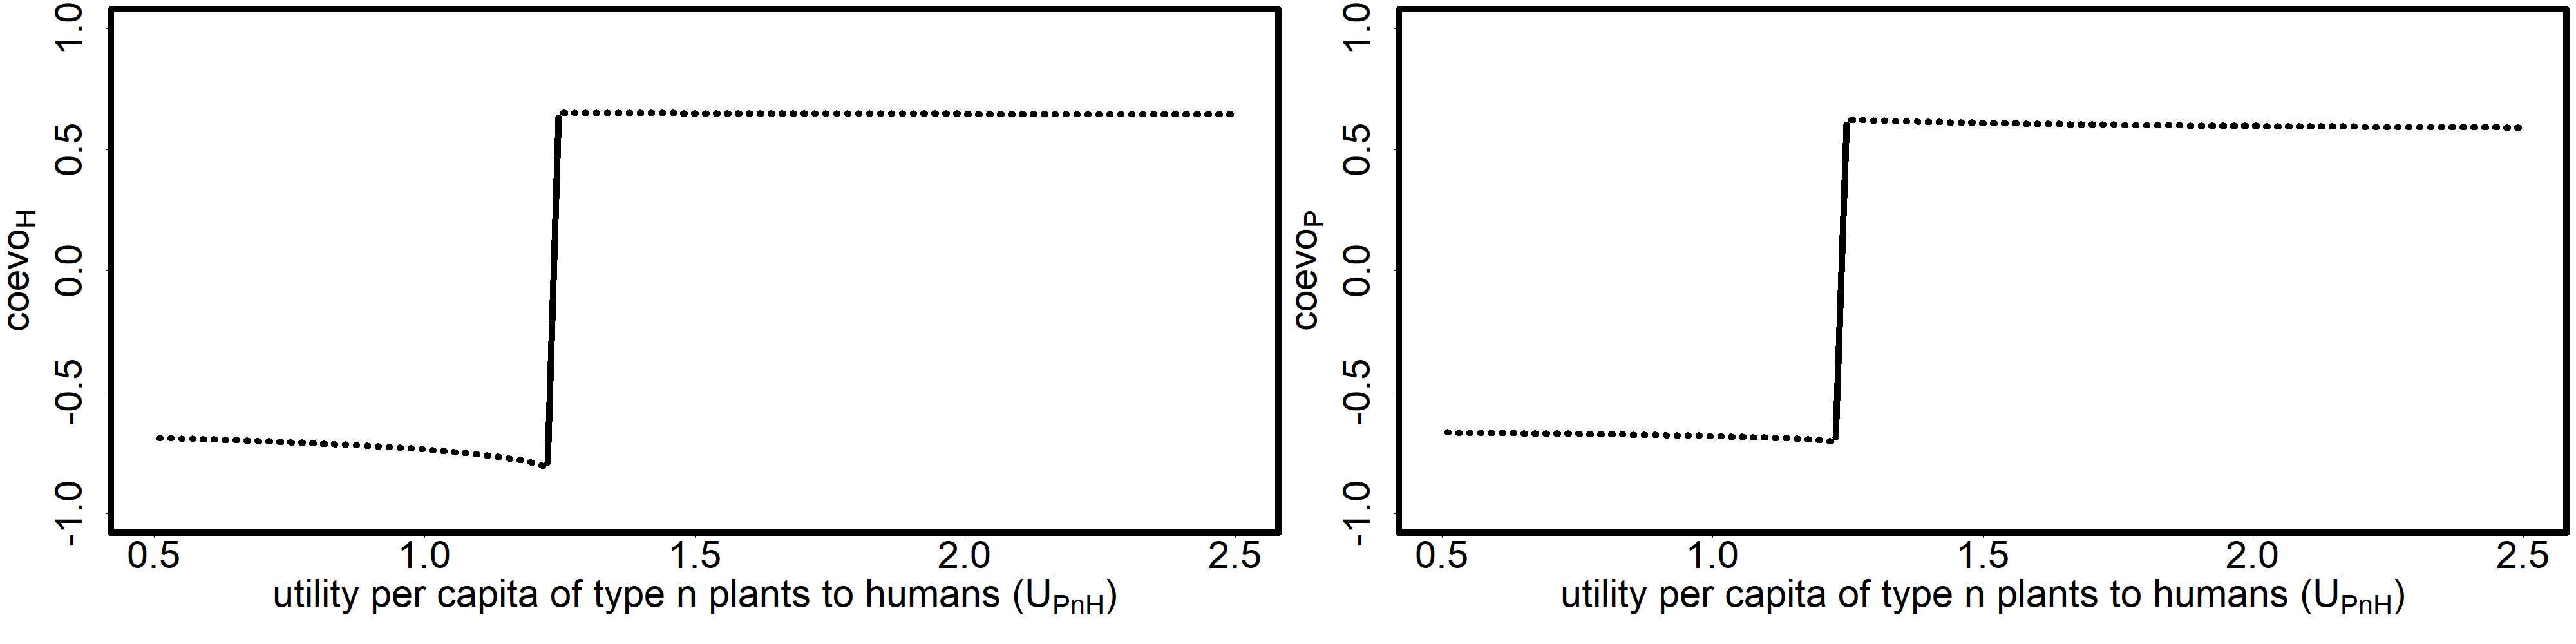
\includegraphics[width=1\linewidth]{plots/2_onePar-mU.PnH_bifplot-pair}

\hypertarget{utility-per-capita-of-type-n-human-to-plants-baru_h_np}{%
\subsection{\texorpdfstring{utility per capita \textbf{of} type n human \textbf{to} plants (\(\bar{U}_{H_{n}P}\)):}{utility per capita of type n human to plants (\textbackslash{}bar\{U\}\_\{H\_\{n\}P\}):}}\label{utility-per-capita-of-type-n-human-to-plants-baru_h_np}}

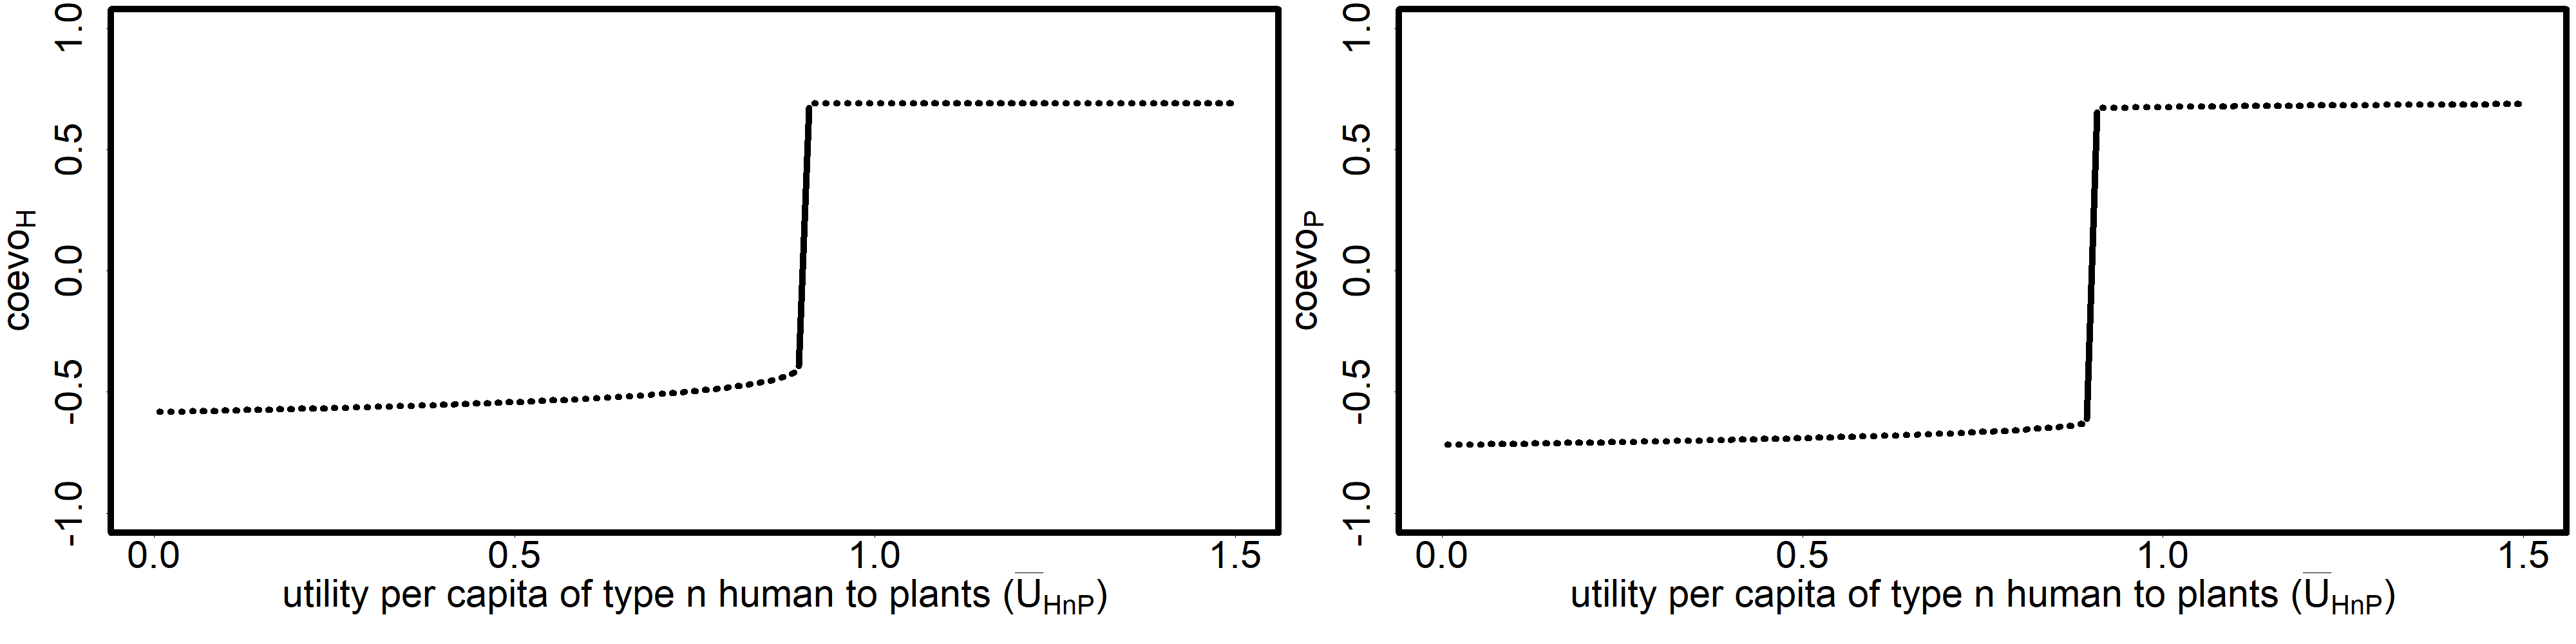
\includegraphics[width=1\linewidth]{plots/2_onePar-mU.HnP_bifplot-pair}

\hypertarget{utility-per-capita-of-type-1-plants-to-humans-baru_p_1h}{%
\subsection{\texorpdfstring{utility per capita \textbf{of} type 1 plants \textbf{to} humans (\(\bar{U}_{P_{1}H}\)):}{utility per capita of type 1 plants to humans (\textbackslash{}bar\{U\}\_\{P\_\{1\}H\}):}}\label{utility-per-capita-of-type-1-plants-to-humans-baru_p_1h}}

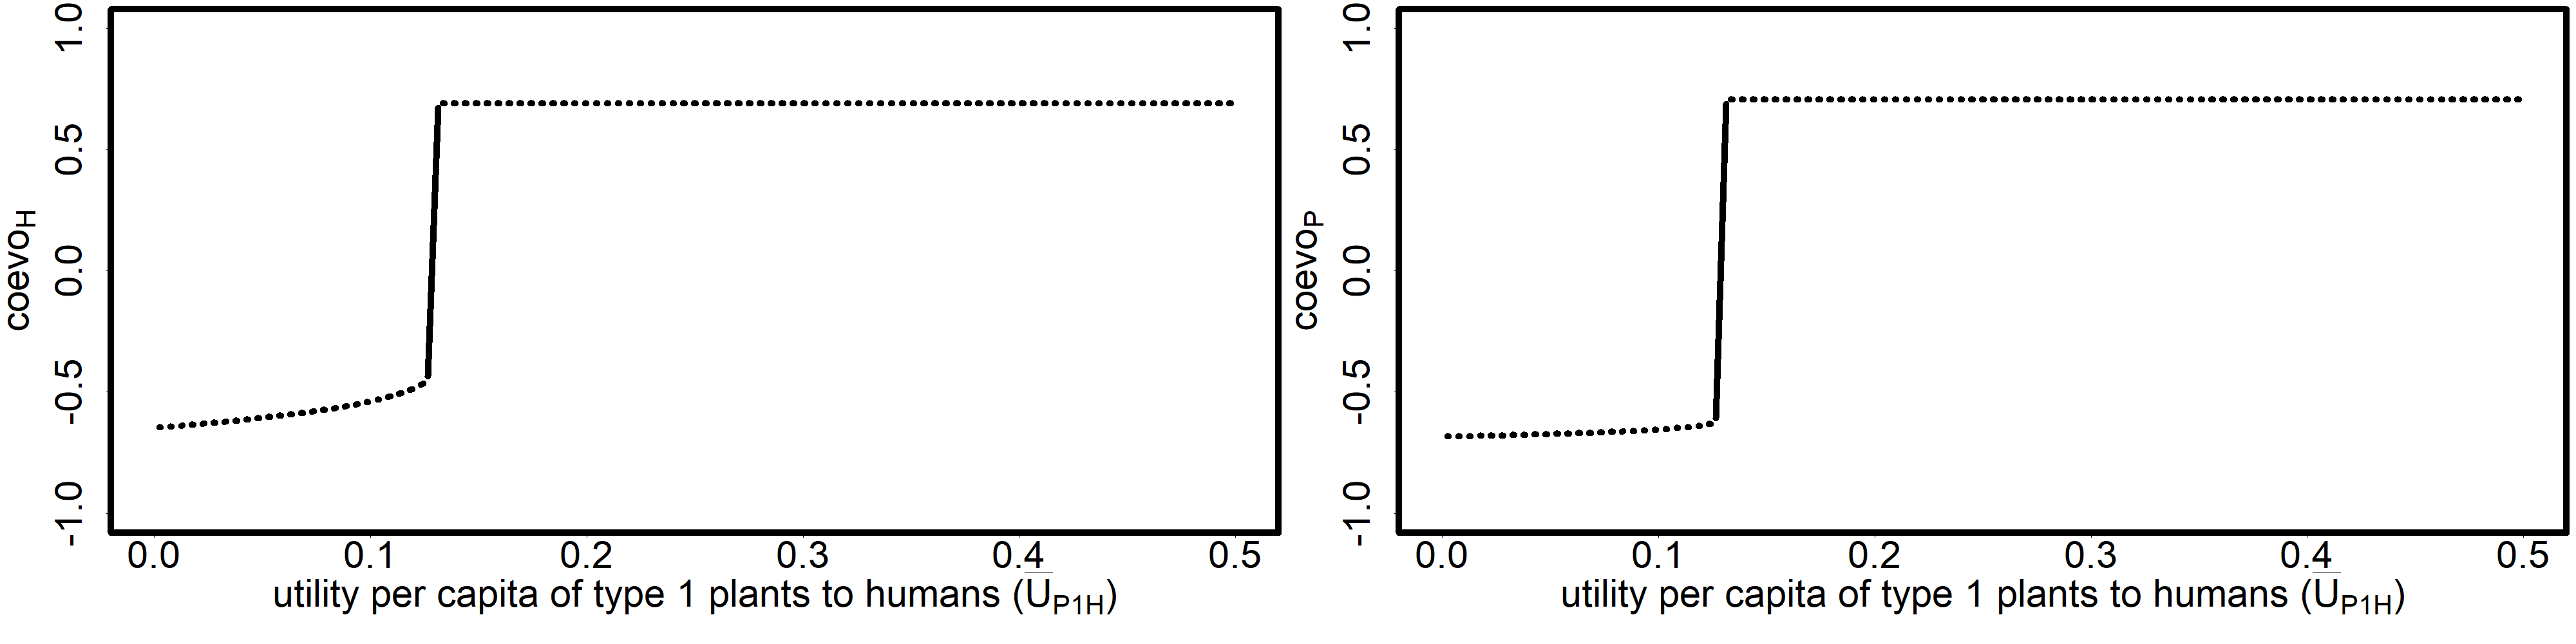
\includegraphics[width=1\linewidth]{plots/2_onePar-mU.P1H_bifplot-pair}

\hypertarget{utility-per-capita-of-type-1-humans-to-plants-baru_h_1p}{%
\subsection{\texorpdfstring{utility per capita \textbf{of} type 1 humans \textbf{to} plants (\(\bar{U}_{H_{1}P}\)):}{utility per capita of type 1 humans to plants (\textbackslash{}bar\{U\}\_\{H\_\{1\}P\}):}}\label{utility-per-capita-of-type-1-humans-to-plants-baru_h_1p}}

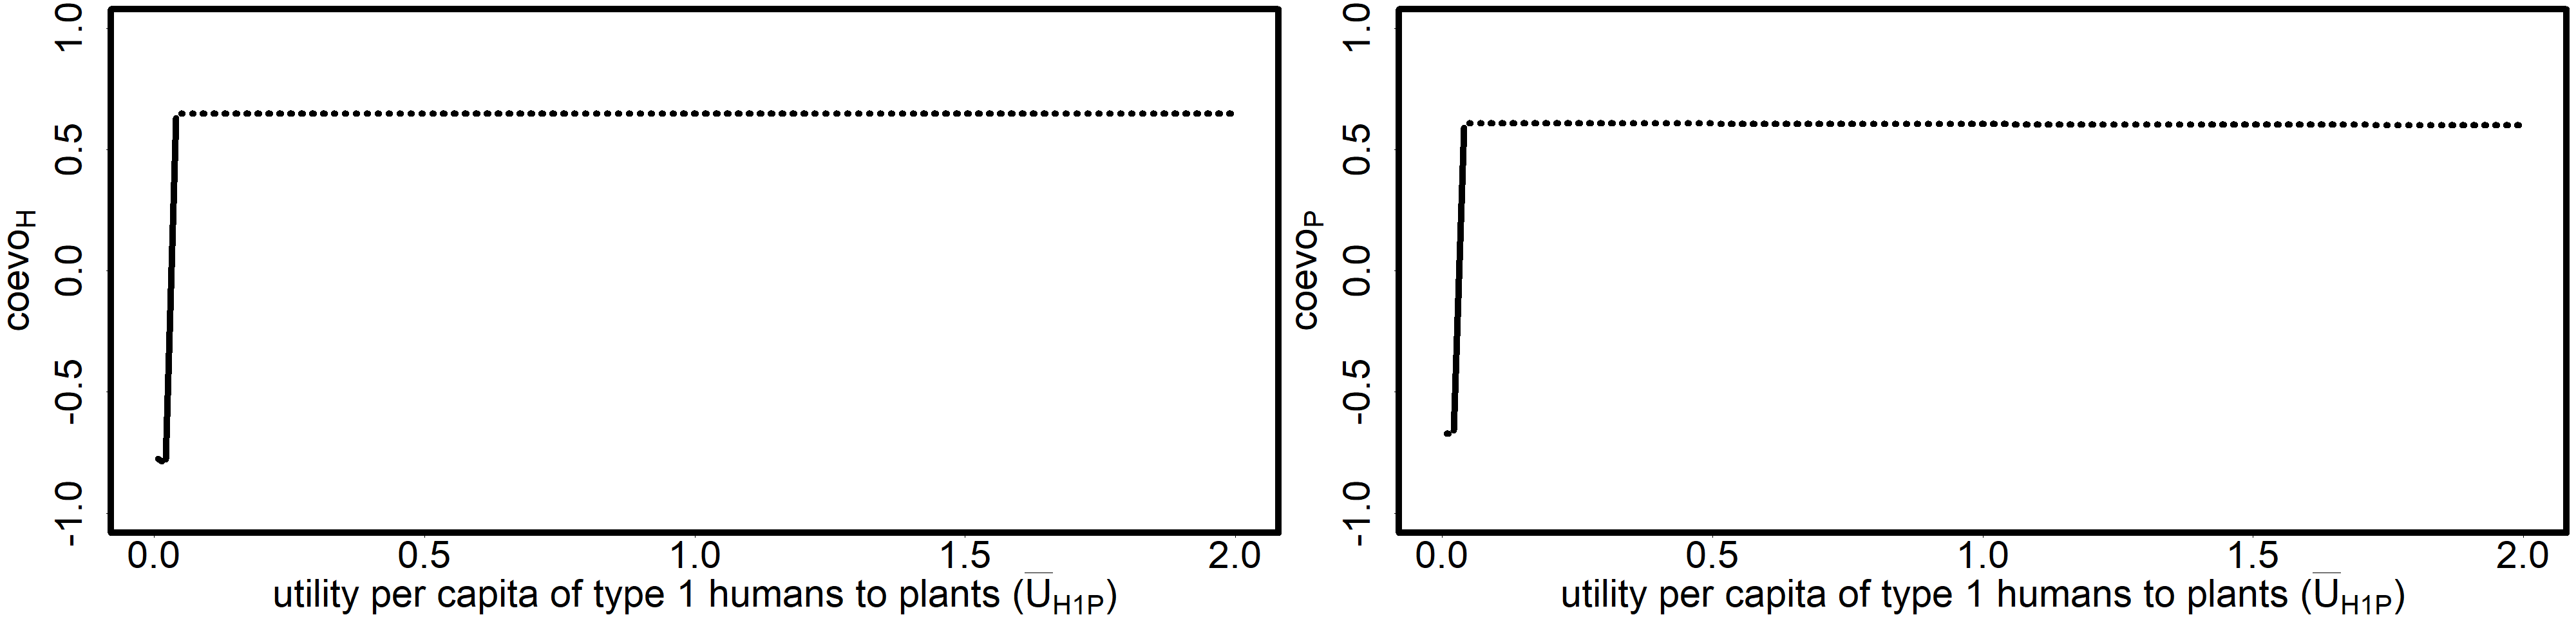
\includegraphics[width=1\linewidth]{plots/2_onePar-mU.H1P_bifplot-pair}

\hypertarget{utility-of-other-resources-to-humans-of-type-1-u_bh_1}{%
\subsection{\texorpdfstring{utility \textbf{of} other resources \textbf{to} humans of type 1 (\(U_{bH_{1}}\)):}{utility of other resources to humans of type 1 (U\_\{bH\_\{1\}\}):}}\label{utility-of-other-resources-to-humans-of-type-1-u_bh_1}}

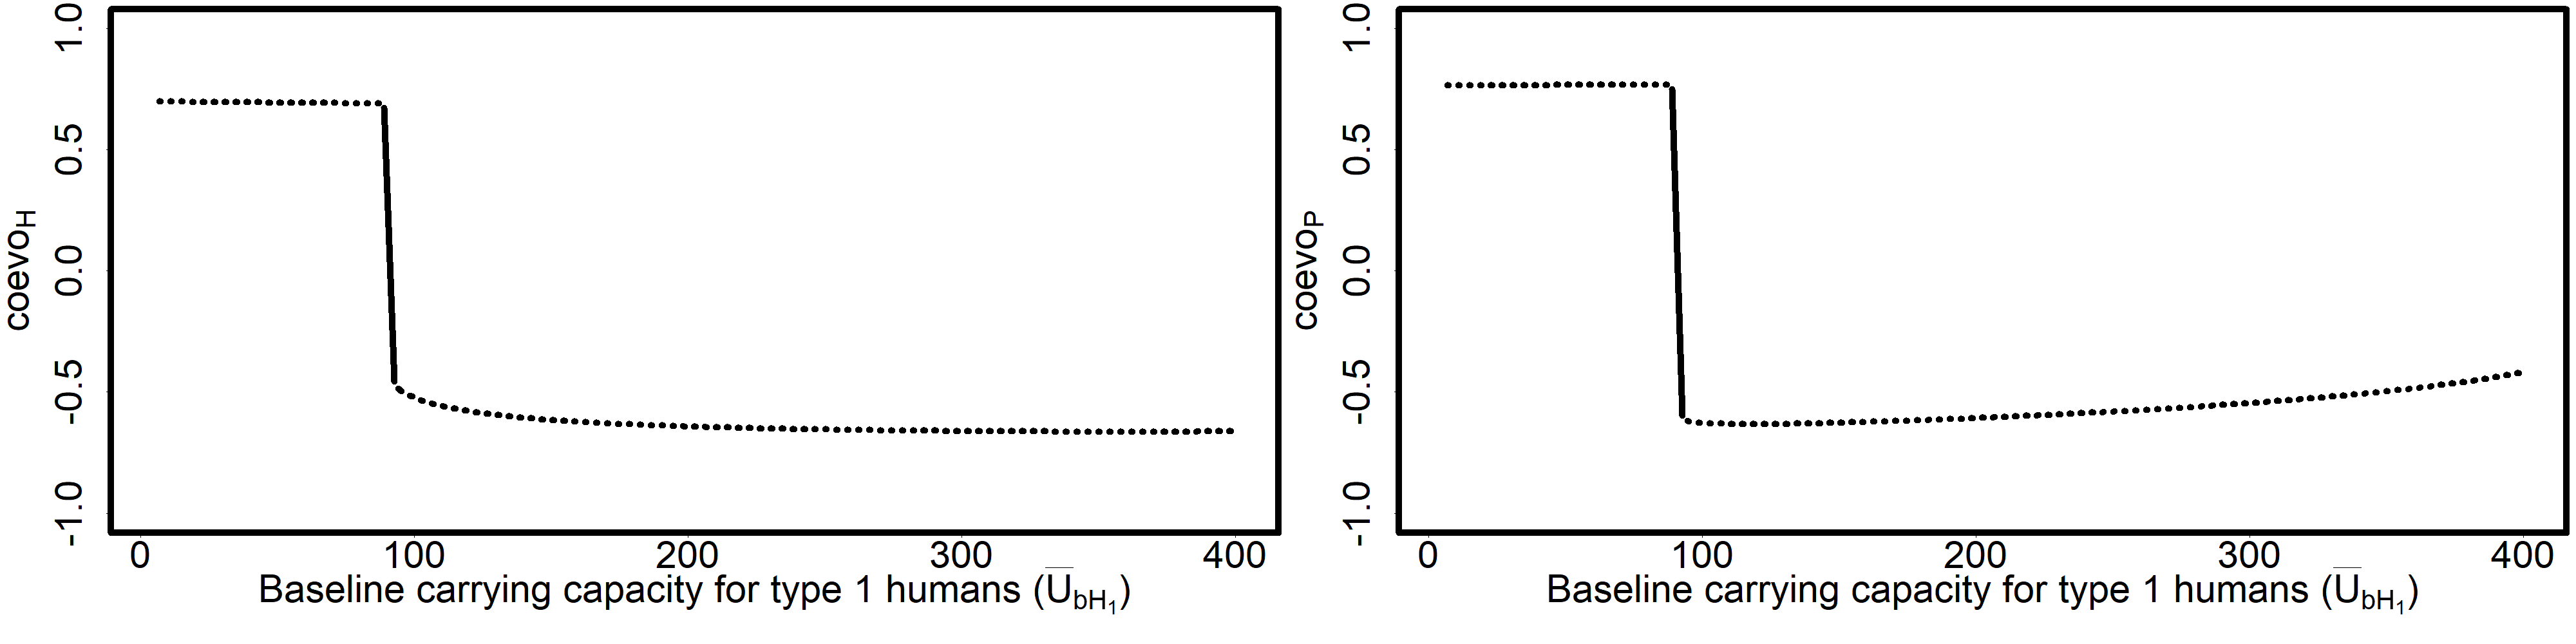
\includegraphics[width=1\linewidth]{plots/2_onePar-U.bH1_bifplot-pair}

\hypertarget{utility-of-non-anthropic-space-to-type-1-plants-u_bp_1}{%
\subsection{\texorpdfstring{utility \textbf{of} non-anthropic space \textbf{to} type 1 plants (\(U_{bP_{1}}\)):}{utility of non-anthropic space to type 1 plants (U\_\{bP\_\{1\}\}):}}\label{utility-of-non-anthropic-space-to-type-1-plants-u_bp_1}}

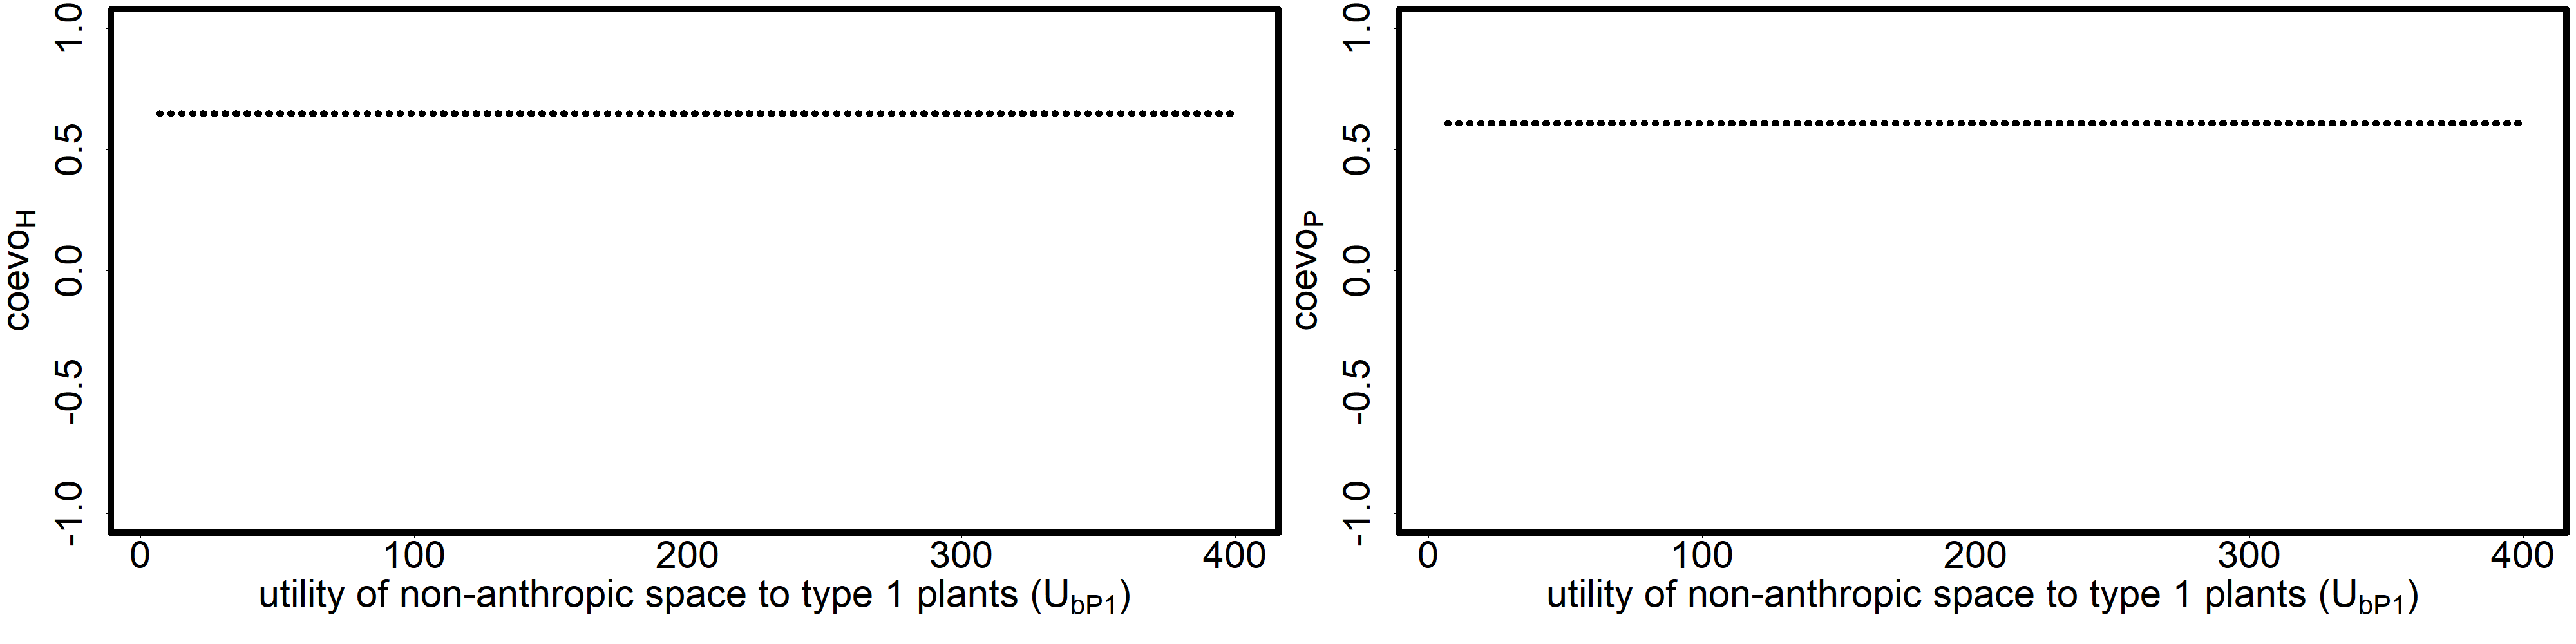
\includegraphics[width=1\linewidth]{plots/2_onePar-U.bP1_bifplot-pair}

\hypertarget{utility-of-other-resources-to-type-n-humans-u_bh_n}{%
\subsection{\texorpdfstring{utility \textbf{of} other resources \textbf{to} type n humans (\(U_{bH_{n}}\)):}{utility of other resources to type n humans (U\_\{bH\_\{n\}\}):}}\label{utility-of-other-resources-to-type-n-humans-u_bh_n}}

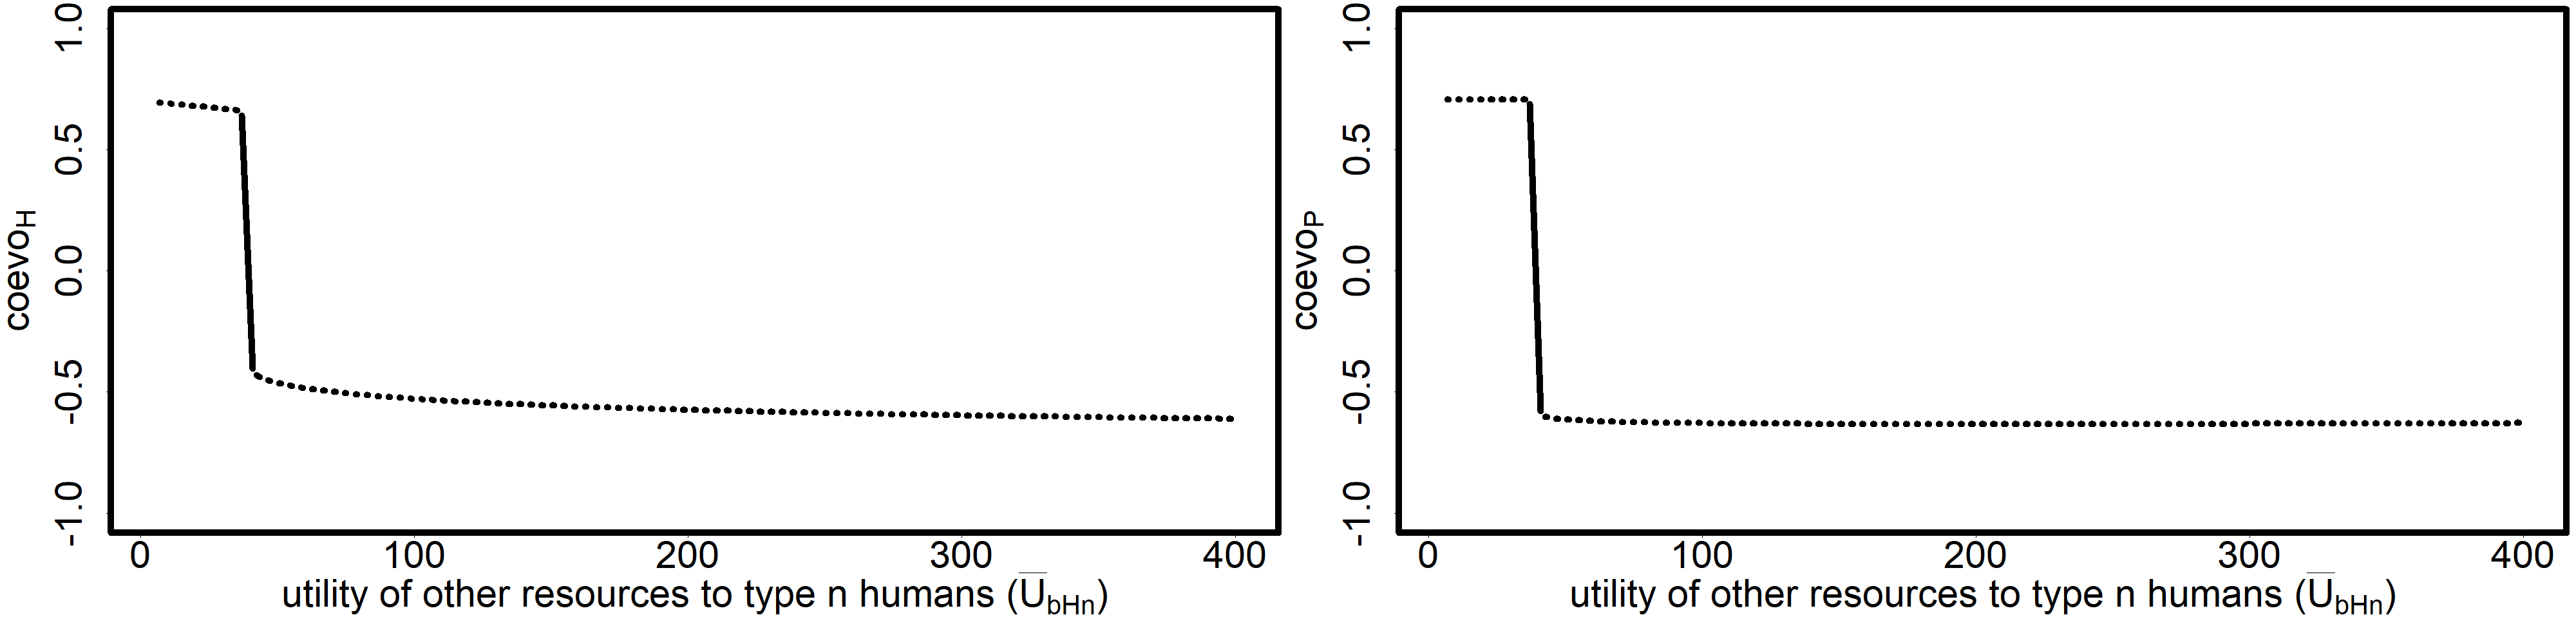
\includegraphics[width=1\linewidth]{plots/2_onePar-U.bHn_bifplot-pair}

\hypertarget{utility-of-non-anthropic-space-to-type-n-plants-u_bp_n}{%
\subsection{\texorpdfstring{utility \textbf{of} non-anthropic space \textbf{to} type n plants (\(U_{bP_{n}}\)):}{utility of non-anthropic space to type n plants (U\_\{bP\_\{n\}\}):}}\label{utility-of-non-anthropic-space-to-type-n-plants-u_bp_n}}

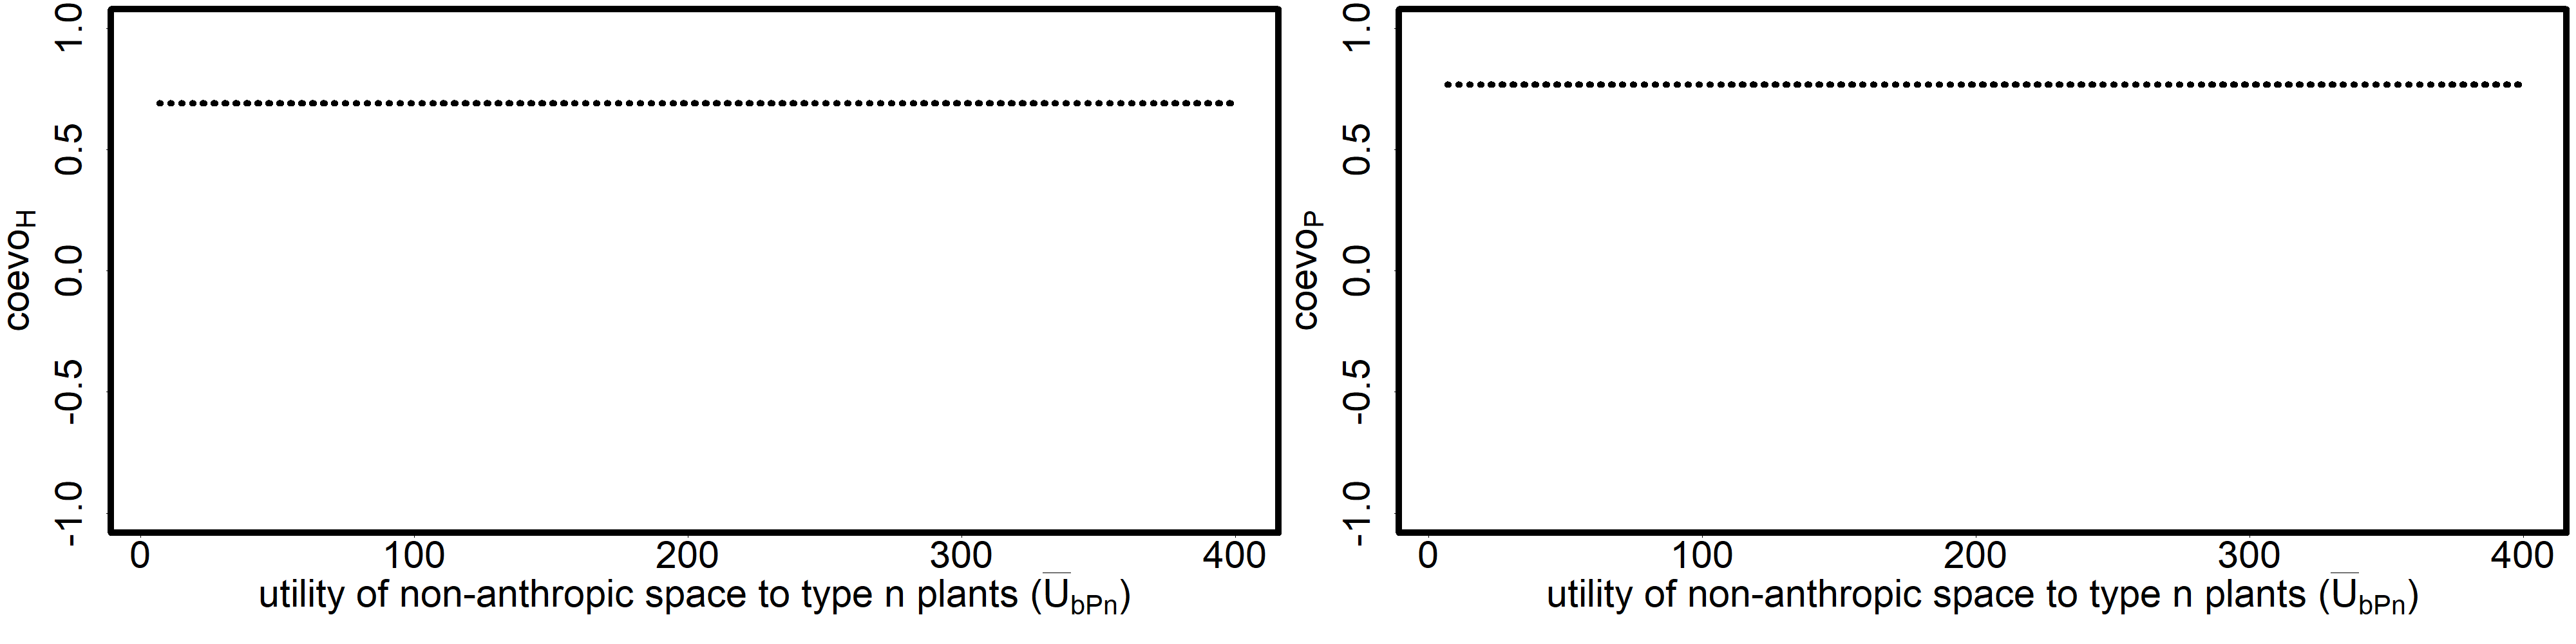
\includegraphics[width=1\linewidth]{plots/2_onePar-U.bPn_bifplot-pair}

\hypertarget{maximum-contiguous-area-to-be-used-by-plants-maxarea}{%
\subsection{\texorpdfstring{maximum contiguous area to be used by plants (\(MaxArea\)):}{maximum contiguous area to be used by plants (MaxArea):}}\label{maximum-contiguous-area-to-be-used-by-plants-maxarea}}

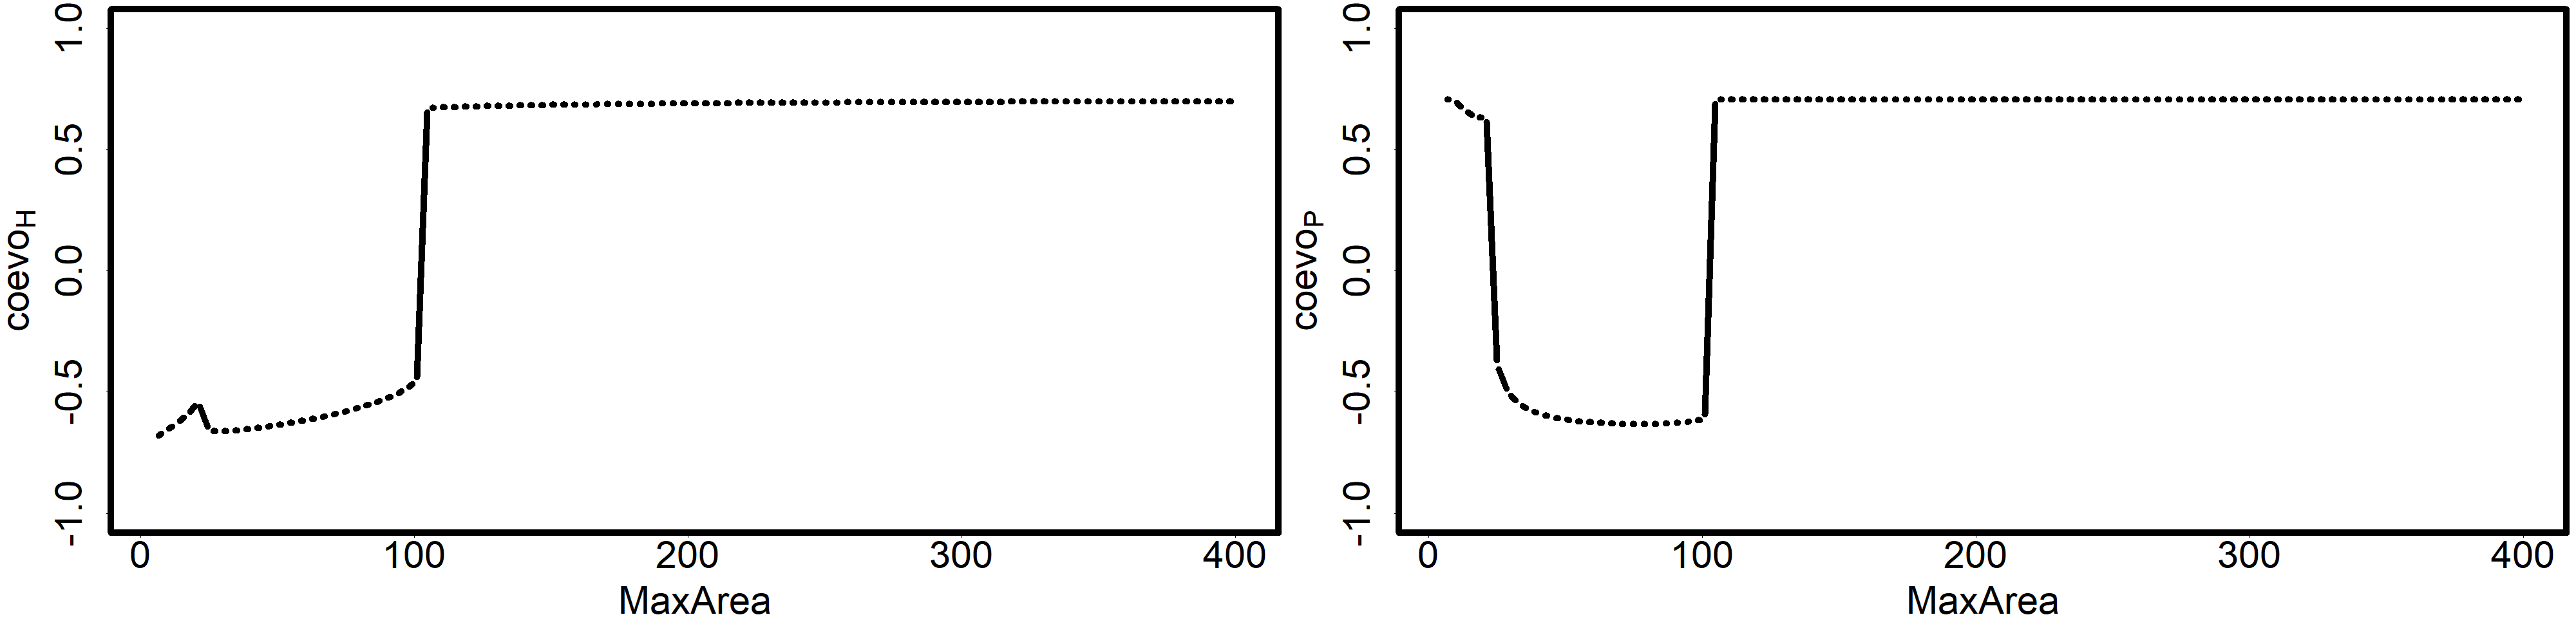
\includegraphics[width=1\linewidth]{plots/2_onePar-MaxArea_bifplot-pair}

\begin{center}\rule{0.5\linewidth}{\linethickness}\end{center}

\hypertarget{oscilations}{%
\section{Oscilations}\label{oscilations}}

Bifurcation plot with last 100 time steps (of 1000) to capture oscillations or `slow' asymptotic stability

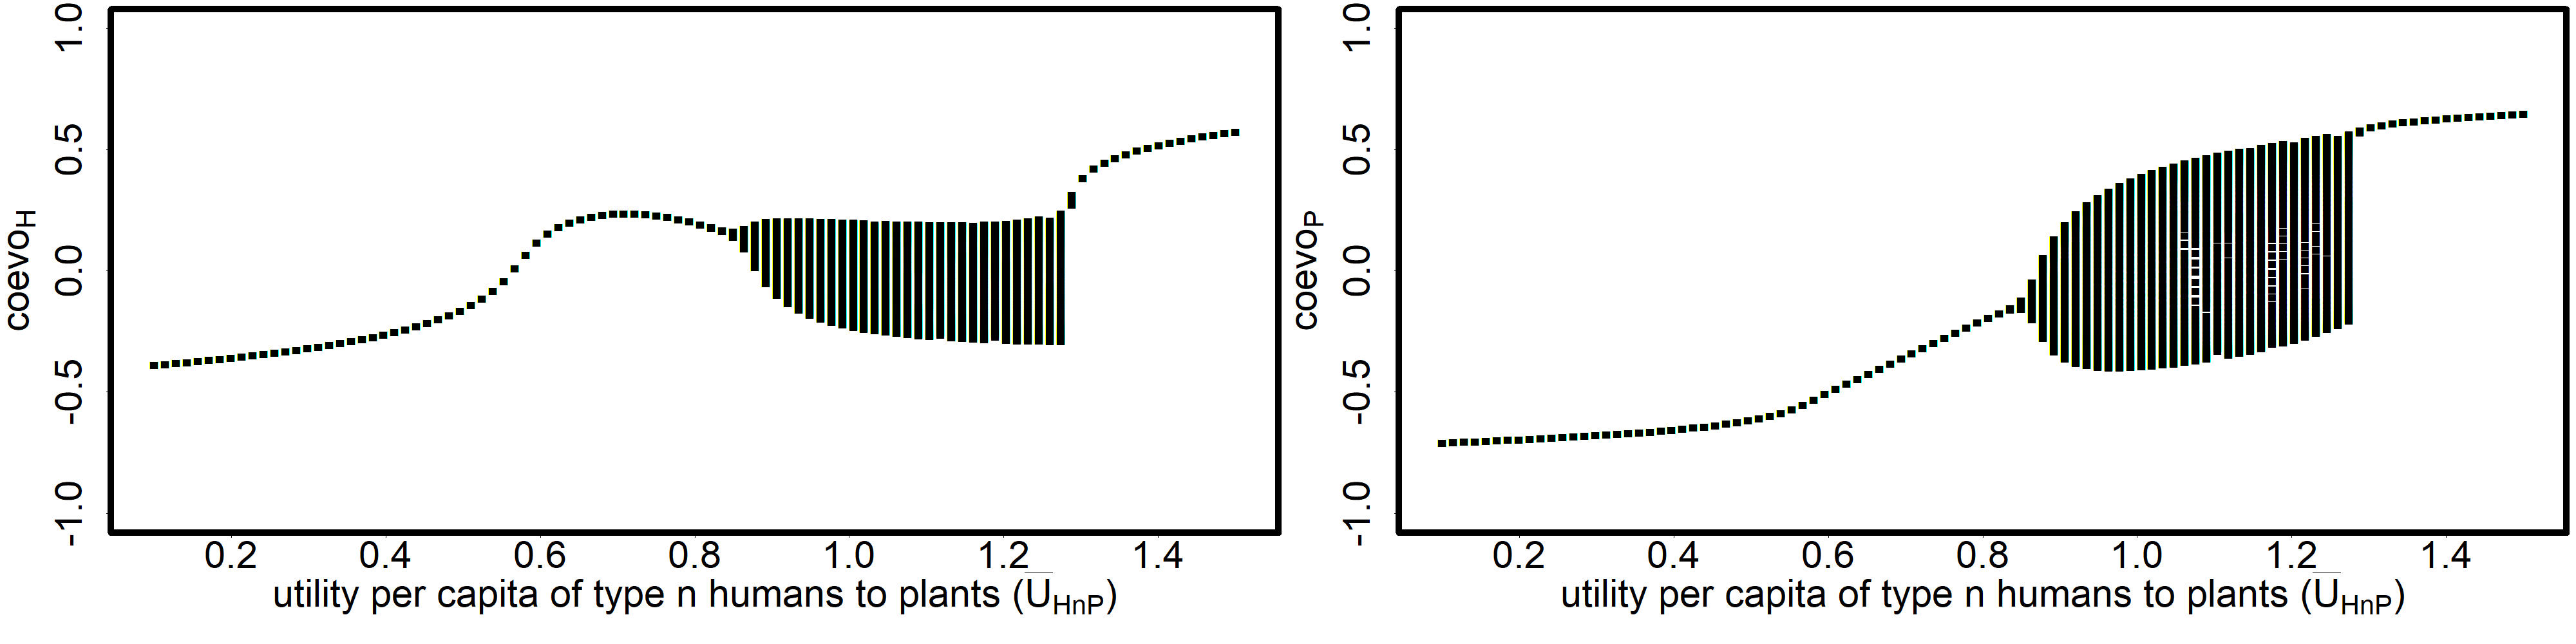
\includegraphics[width=1\linewidth]{plots/2_onePar-mU.HnP.osc_bifplot-pair}

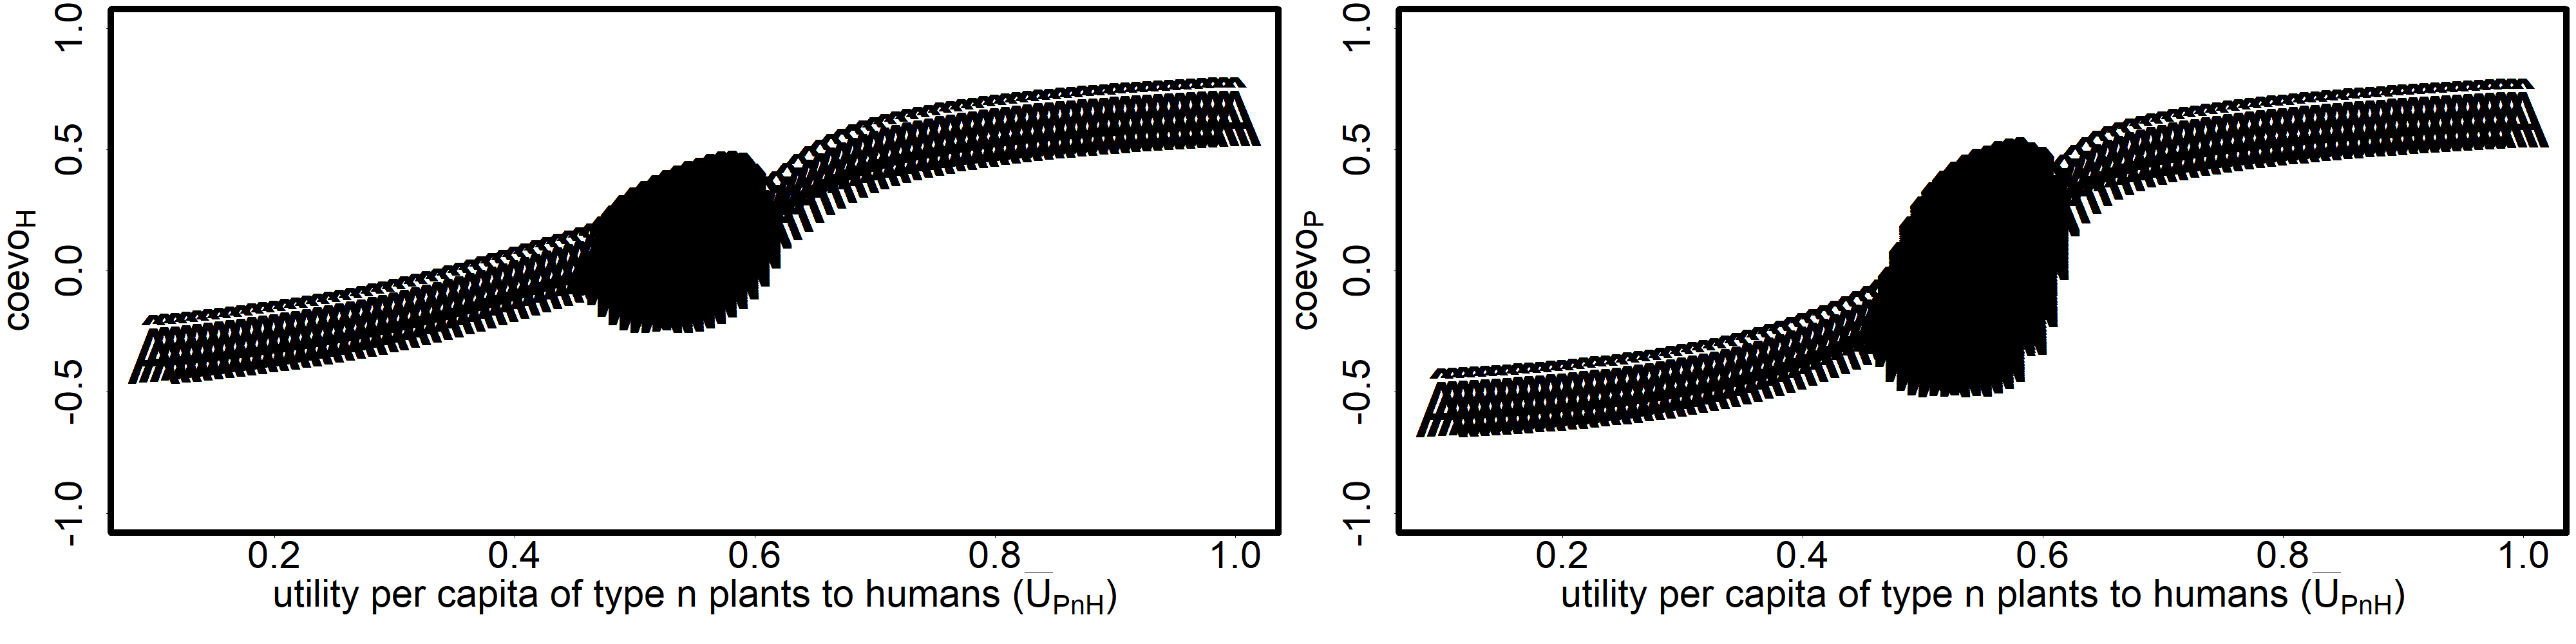
\includegraphics[width=1\linewidth]{plots/2_onePar-mU.PnH.osc_bifplot-pair}

\hypertarget{two-parameter-exploration}{%
\chapter{Two parameter exploration}\label{two-parameter-exploration}}

\hypertarget{full-example}{%
\section{Full example}\label{full-example}}

\hypertarget{utility-per-capita-from-type-n-humans-and-plants-baru_h_np-x-baru_p_nh}{%
\subsection{\texorpdfstring{Utility per capita from type n humans and plants (\(\bar{U}_{H_{n}P}\) x \(\bar{U}_{P_{n}H}\)):}{Utility per capita from type n humans and plants (\textbackslash{}bar\{U\}\_\{H\_\{n\}P\} x \textbackslash{}bar\{U\}\_\{P\_\{n\}H\}):}}\label{utility-per-capita-from-type-n-humans-and-plants-baru_h_np-x-baru_p_nh}}

\begin{tabular}{l|l}
\hline
parameter & value\\
\hline
iniH & 10\\
\hline
iniP & 10\\
\hline
n.H & 30\\
\hline
n.P & 30\\
\hline
v.H & 0.15\\
\hline
v.P & 0.15\\
\hline
r.H & 0.04\\
\hline
r.P & 0.1\\
\hline
mU.PnH & 0 - 2.5 (sample = 15 )\\
\hline
mU.HnP & 0 - 2.5 (sample = 15 )\\
\hline
mU.P1H & 0.15\\
\hline
mU.H1P & 0\\
\hline
U.bHn & 10\\
\hline
U.bPn & 20\\
\hline
U.bH1 & 80\\
\hline
U.bP1 & 100\\
\hline
MaxArea & 200\\
\hline
\end{tabular}

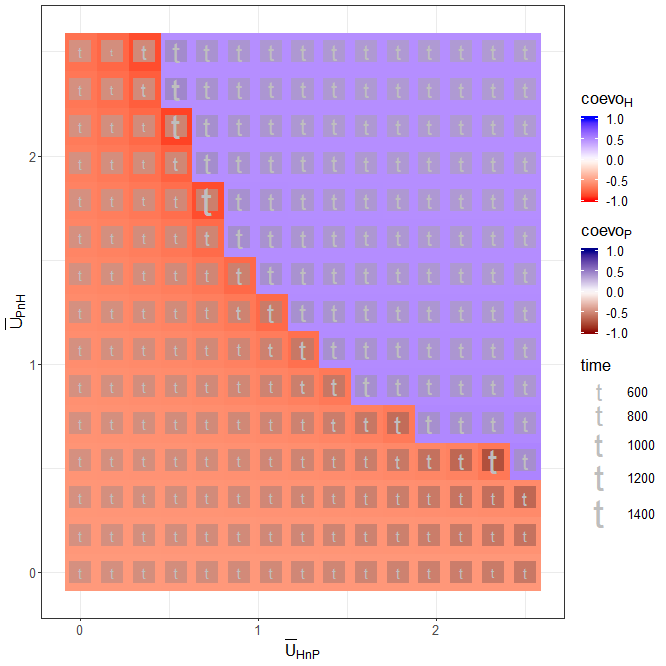
\includegraphics[width=1\linewidth]{plots/3_twoPar-mU.HnP-mU.PnH_plot}

\begin{center}\rule{0.5\linewidth}{\linethickness}\end{center}

\hypertarget{exploration-on-default-setting-for-directly-related-parameter-pairs}{%
\section{Exploration on `default' setting for (directly-related) parameter pairs:}\label{exploration-on-default-setting-for-directly-related-parameter-pairs}}

\hypertarget{number-of-types-of-humans-and-plants-n_h-x-n_p}{%
\subsection{\texorpdfstring{Number of types of humans and plants (\(n_{H}\) x \(n_{P}\)):}{Number of types of humans and plants (n\_\{H\} x n\_\{P\}):}}\label{number-of-types-of-humans-and-plants-n_h-x-n_p}}

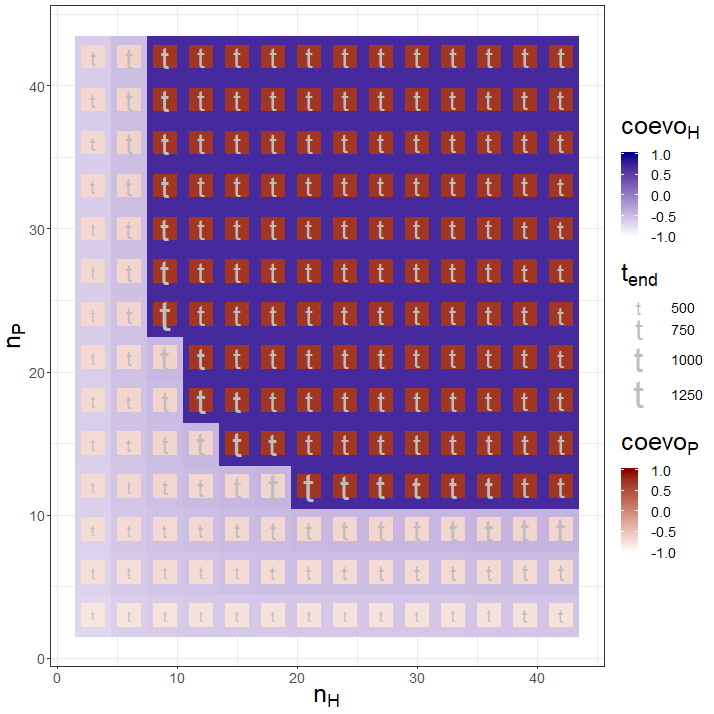
\includegraphics[width=1\linewidth]{plots/3_twoPar-n.H-n.P_plot}

\hypertarget{undirected-variation-in-humans-and-plants-v_h-x-v_p}{%
\subsection{\texorpdfstring{Undirected variation in humans and plants (\(v_{H}\) x \(v_{P}\)):}{Undirected variation in humans and plants (v\_\{H\} x v\_\{P\}):}}\label{undirected-variation-in-humans-and-plants-v_h-x-v_p}}

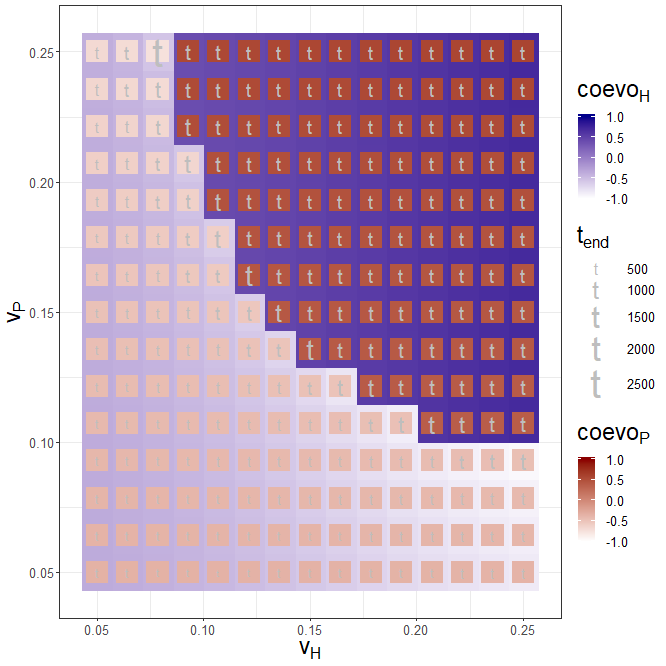
\includegraphics[width=1\linewidth]{plots/3_twoPar-v.H-v.P_plot}

\hypertarget{utility-per-capita-from-type-1-humans-and-plants-baru_h_1p-x-baru_p_1h}{%
\subsection{\texorpdfstring{Utility per capita from type 1 humans and plants (\(\bar{U}_{H_{1}P}\) x \(\bar{U}_{P_{1}H}\)):}{Utility per capita from type 1 humans and plants (\textbackslash{}bar\{U\}\_\{H\_\{1\}P\} x \textbackslash{}bar\{U\}\_\{P\_\{1\}H\}):}}\label{utility-per-capita-from-type-1-humans-and-plants-baru_h_1p-x-baru_p_1h}}

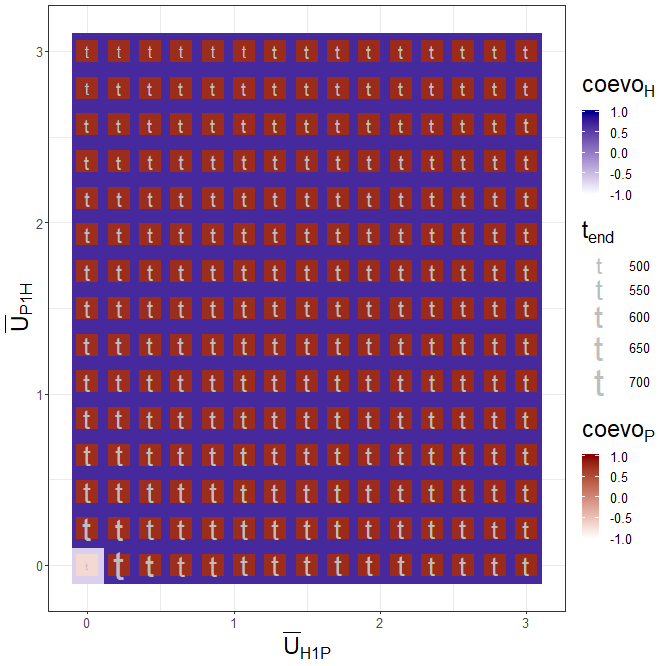
\includegraphics[width=1\linewidth]{plots/3_twoPar-mU.H1P-mU.P1H_plot}

\hypertarget{utility-per-capita-from-type-n-humans-and-plants-baru_h_np-x-baru_p_nh-1}{%
\subsection{\texorpdfstring{Utility per capita from type n humans and plants (\(\bar{U}_{H_{n}P}\) x \(\bar{U}_{P_{n}H}\)):}{Utility per capita from type n humans and plants (\textbackslash{}bar\{U\}\_\{H\_\{n\}P\} x \textbackslash{}bar\{U\}\_\{P\_\{n\}H\}):}}\label{utility-per-capita-from-type-n-humans-and-plants-baru_h_np-x-baru_p_nh-1}}

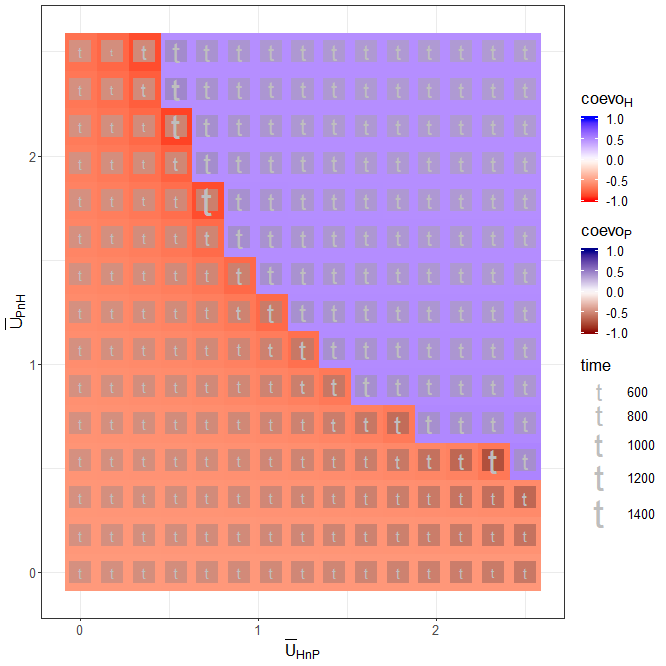
\includegraphics[width=1\linewidth]{plots/3_twoPar-mU.HnP-mU.PnH_plot}

\hypertarget{utility-per-capita-from-humans-to-plants-baru_h_1p-x-baru_h_np}{%
\subsection{\texorpdfstring{Utility per capita from humans to plants (\(\bar{U}_{H_{1}P}\) x \(\bar{U}_{H_{n}P}\)):}{Utility per capita from humans to plants (\textbackslash{}bar\{U\}\_\{H\_\{1\}P\} x \textbackslash{}bar\{U\}\_\{H\_\{n\}P\}):}}\label{utility-per-capita-from-humans-to-plants-baru_h_1p-x-baru_h_np}}

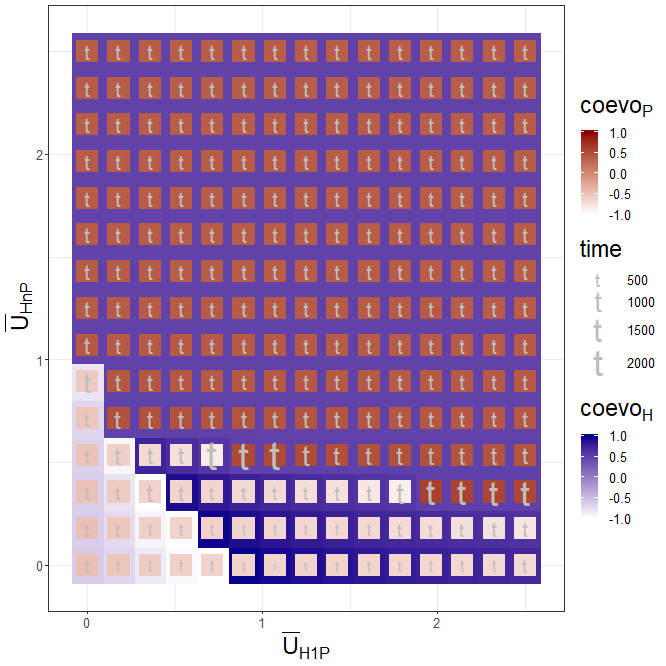
\includegraphics[width=1\linewidth]{plots/3_twoPar-mU.H1P-mU.HnP_plot}

\hypertarget{utility-per-capita-from-plants-to-humans-baru_p_1h-x-baru_p_nh}{%
\subsection{\texorpdfstring{Utility per capita from plants to humans (\(\bar{U}_{P_{1}H}\) x \(\bar{U}_{P_{n}H}\)):}{Utility per capita from plants to humans (\textbackslash{}bar\{U\}\_\{P\_\{1\}H\} x \textbackslash{}bar\{U\}\_\{P\_\{n\}H\}):}}\label{utility-per-capita-from-plants-to-humans-baru_p_1h-x-baru_p_nh}}

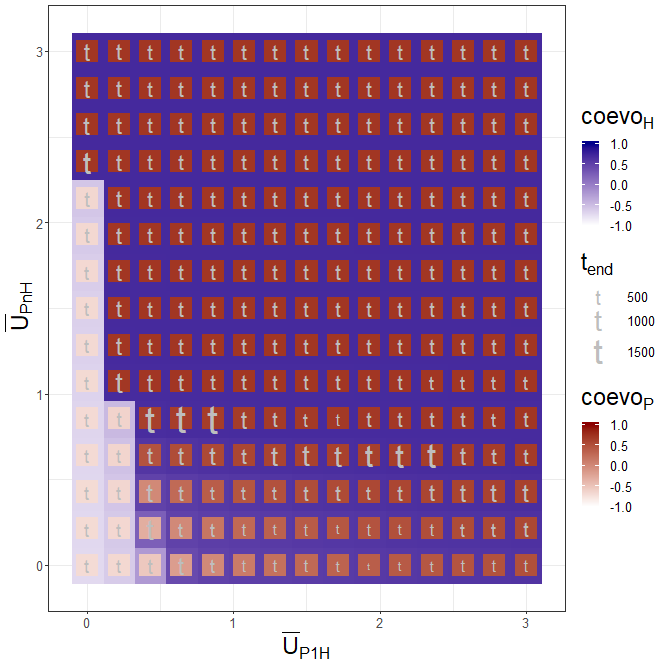
\includegraphics[width=1\linewidth]{plots/3_twoPar-mU.P1H-mU.PnH_plot}

\hypertarget{utility-of-other-resources-to-type-1-humans-and-plants-u_bh_1-x-u_bp_1}{%
\subsection{\texorpdfstring{Utility of other resources to type 1 humans and plants (\(U_{bH_{1}}\) x \(U_{bP_{1}}\)):}{Utility of other resources to type 1 humans and plants (U\_\{bH\_\{1\}\} x U\_\{bP\_\{1\}\}):}}\label{utility-of-other-resources-to-type-1-humans-and-plants-u_bh_1-x-u_bp_1}}

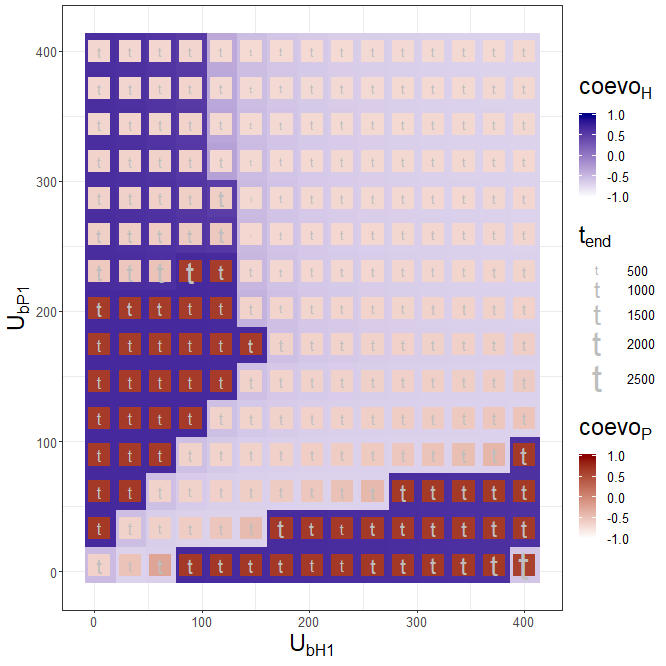
\includegraphics[width=1\linewidth]{plots/3_twoPar-U.bH1-U.bP1_plot}

\hypertarget{utility-of-other-resources-to-type-n-humans-and-plants-u_bh_n-x-u_bp_n}{%
\subsection{\texorpdfstring{Utility of other resources to type n humans and plants (\(U_{bH_{n}}\) x \(U_{bP_{n}}\)):}{Utility of other resources to type n humans and plants (U\_\{bH\_\{n\}\} x U\_\{bP\_\{n\}\}):}}\label{utility-of-other-resources-to-type-n-humans-and-plants-u_bh_n-x-u_bp_n}}

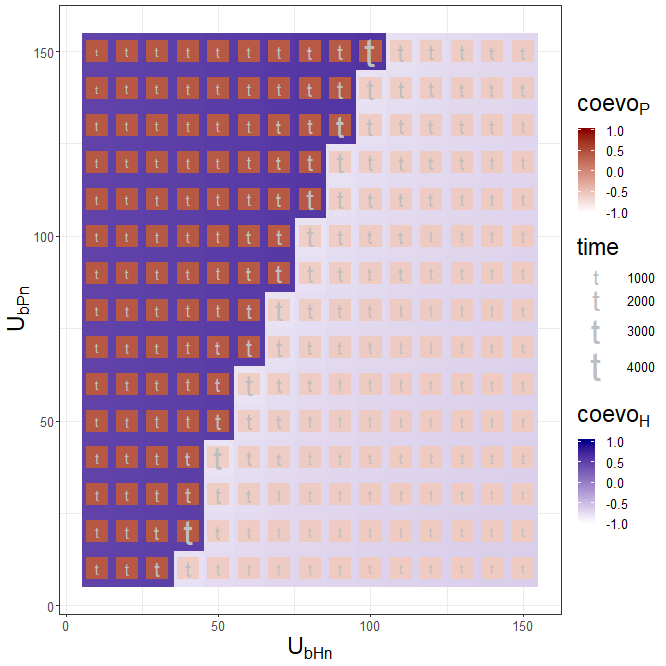
\includegraphics[width=1\linewidth]{plots/3_twoPar-U.bHn-U.bPn_plot}

\hypertarget{utility-of-other-resources-to-humans-u_bh_1-x-u_bh_n}{%
\subsection{\texorpdfstring{Utility of other resources to humans (\(U_{bH_{1}}\) x \(U_{bH_{n}}\)):}{Utility of other resources to humans (U\_\{bH\_\{1\}\} x U\_\{bH\_\{n\}\}):}}\label{utility-of-other-resources-to-humans-u_bh_1-x-u_bh_n}}

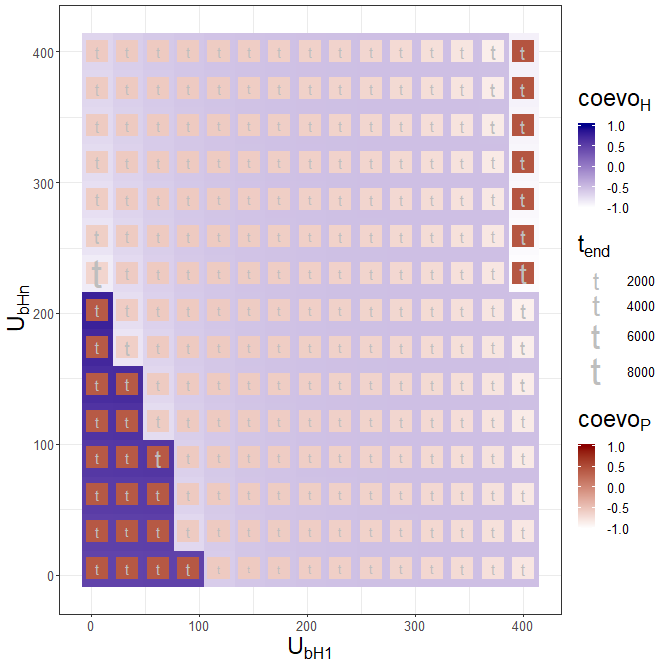
\includegraphics[width=1\linewidth]{plots/3_twoPar-U.bH1-U.bHn_plot}

\hypertarget{utility-of-other-resources-to-plants-u_bp_1-x-u_bp_n}{%
\subsection{\texorpdfstring{Utility of other resources to plants (\(U_{bP_{1}}\) x \(U_{bP_{n}}\)):}{Utility of other resources to plants (U\_\{bP\_\{1\}\} x U\_\{bP\_\{n\}\}):}}\label{utility-of-other-resources-to-plants-u_bp_1-x-u_bp_n}}

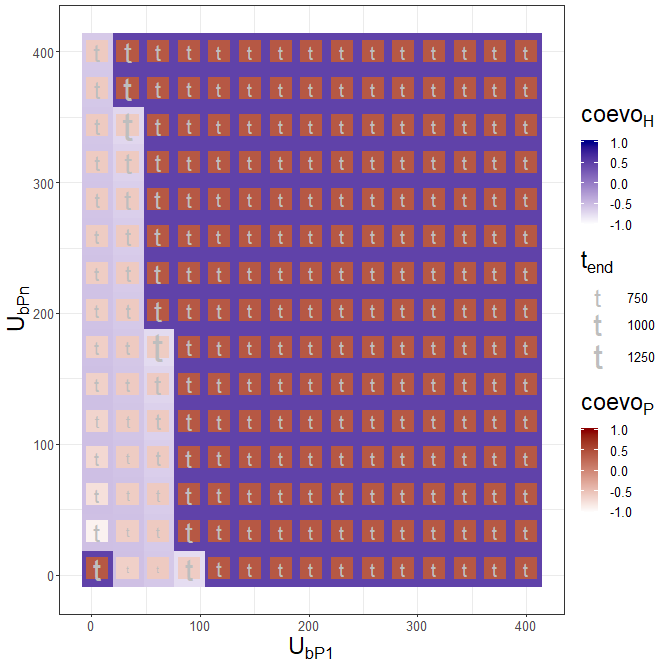
\includegraphics[width=1\linewidth]{plots/3_twoPar-U.bP1-U.bPn_plot}

\hypertarget{four-parameter-exploration}{%
\chapter{Four parameter exploration}\label{four-parameter-exploration}}

\hypertarget{utility-per-capita-between-humans-and-plants-baru_h_1p-x-baru_p_1h-x-baru_h_np-x-baru_p_nh}{%
\section{\texorpdfstring{Utility per capita between humans and plants (\(\bar{U}_{H_{1}P}\) x \(\bar{U}_{P_{1}H}\) x \(\bar{U}_{H_{n}P}\) x \(\bar{U}_{P_{n}H}\))}{Utility per capita between humans and plants (\textbackslash{}bar\{U\}\_\{H\_\{1\}P\} x \textbackslash{}bar\{U\}\_\{P\_\{1\}H\} x \textbackslash{}bar\{U\}\_\{H\_\{n\}P\} x \textbackslash{}bar\{U\}\_\{P\_\{n\}H\})}}\label{utility-per-capita-between-humans-and-plants-baru_h_1p-x-baru_p_1h-x-baru_h_np-x-baru_p_nh}}

\begin{tabular}{l|l}
\hline
parameter & value\\
\hline
iniH & 10\\
\hline
iniP & 10\\
\hline
n.H & 30\\
\hline
n.P & 30\\
\hline
v.H & 0.15\\
\hline
v.P & 0.15\\
\hline
r.H & 0.04\\
\hline
r.P & 0.1\\
\hline
mU.PnH & 0 - 2.5 (sample = 5 )\\
\hline
mU.HnP & 0 - 2.5 (sample = 5 )\\
\hline
mU.P1H & 0 - 2.5 (sample = 5 )\\
\hline
mU.H1P & 0 - 2.5 (sample = 5 )\\
\hline
U.bHn & 10\\
\hline
U.bPn & 20\\
\hline
U.bH1 & 80\\
\hline
U.bP1 & 100\\
\hline
MaxArea & 200\\
\hline
\end{tabular}

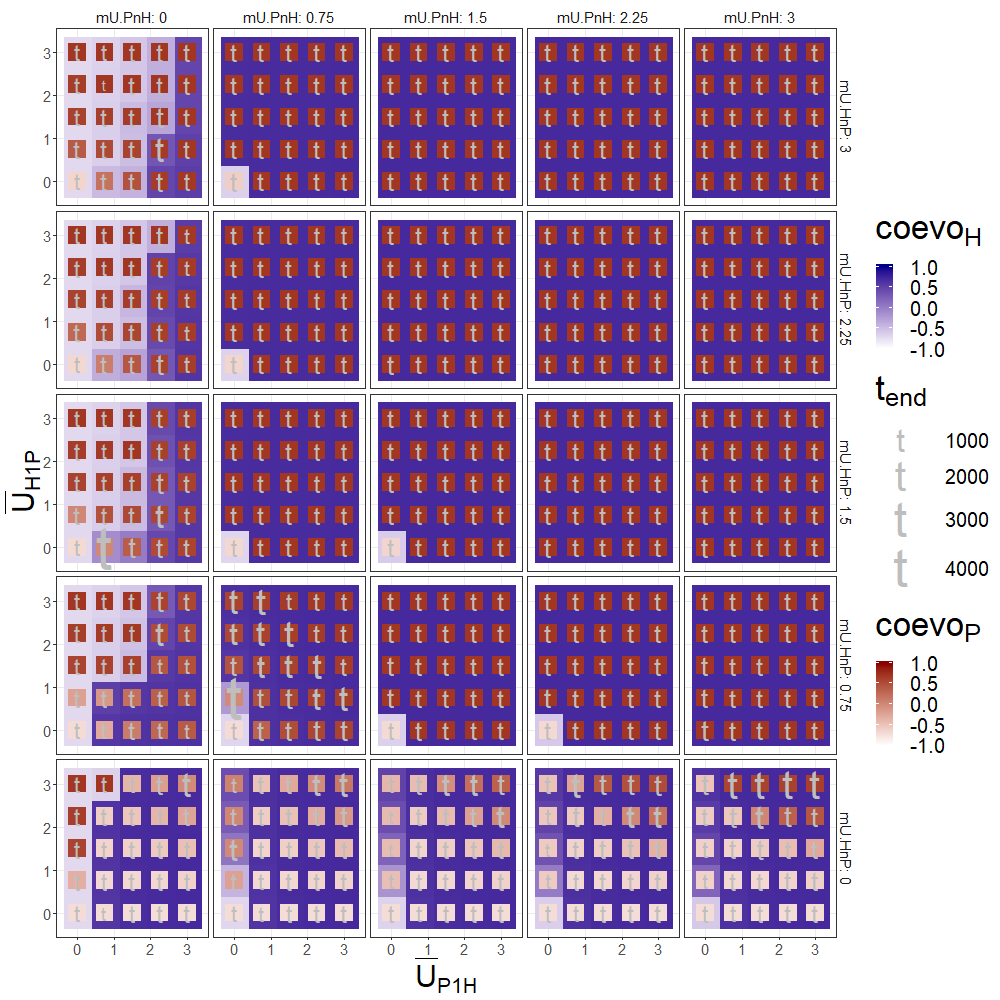
\includegraphics[width=1\linewidth]{plots/4_fourPar-mU.HP-mU.PH_plot}

\textbf{\emph{Interpretation}}:\\
* Higher values of all four parameters facilitate coevolution; under the `default' setting, a value around 1 is enough for all four parameters (intermediate values in this exploration).\\
* Coevolution is still possible if any single one of these parameters equal zero (bottom-left corners). Under this type of conditions, agriculture (blue) appears more probable than domestication (red), and the latter is strongly dependent on a non-null \(\bar{U}_{H_{n}P}\).\\
* As a summary of possible end-states:\\
+ \emph{`Fast' coevolution} (red square in blue tile, small \emph{t}): most cases when values are greater than 0.625.\\
+ \emph{Domestication without cultivation} (red square in whitish tile): most cases when \(\bar{U}_{H_{n}P}>0.625\), \(\bar{U}_{H_{1}P}\geq 0.625\), \(\bar{U}_{P_{n}H}=0\), and \(\bar{U}_{P_{1}H}<2.5\).\\
+ \emph{Cultivation without domestication} (whitish square in blue tile): most cases when \(\bar{U}_{H_{n}P} = 0\).

\hypertarget{utility-from-other-resources-to-humans-and-plants-u_bh_1-x-u_bp_1-x-u_bh_n-x-u_bp_n}{%
\section{\texorpdfstring{Utility from other resources to humans and plants (\(U_{bH_{1}}\) x \(U_{bP_{1}}\) x \(U_{bH_{n}}\) x \(U_{bP_{n}}\))}{Utility from other resources to humans and plants (U\_\{bH\_\{1\}\} x U\_\{bP\_\{1\}\} x U\_\{bH\_\{n\}\} x U\_\{bP\_\{n\}\})}}\label{utility-from-other-resources-to-humans-and-plants-u_bh_1-x-u_bp_1-x-u_bh_n-x-u_bp_n}}

For this experiment, consider that the default setting includes \(MaxArea=200\) (i.e.~the maximum for the plant population).

\begin{tabular}{l|l}
\hline
parameter & value\\
\hline
iniH & 10\\
\hline
iniP & 10\\
\hline
n.H & 30\\
\hline
n.P & 30\\
\hline
v.H & 0.15\\
\hline
v.P & 0.15\\
\hline
r.H & 0.04\\
\hline
r.P & 0.1\\
\hline
mU.PnH & 1.5\\
\hline
mU.HnP & 1\\
\hline
mU.P1H & 0.15\\
\hline
mU.H1P & 0\\
\hline
U.bHn & 5 - 300 (sample = 5 )\\
\hline
U.bPn & 5 - 300 (sample = 5 )\\
\hline
U.bH1 & 5 - 300 (sample = 5 )\\
\hline
U.bP1 & 5 - 300 (sample = 5 )\\
\hline
MaxArea & 200\\
\hline
\end{tabular}

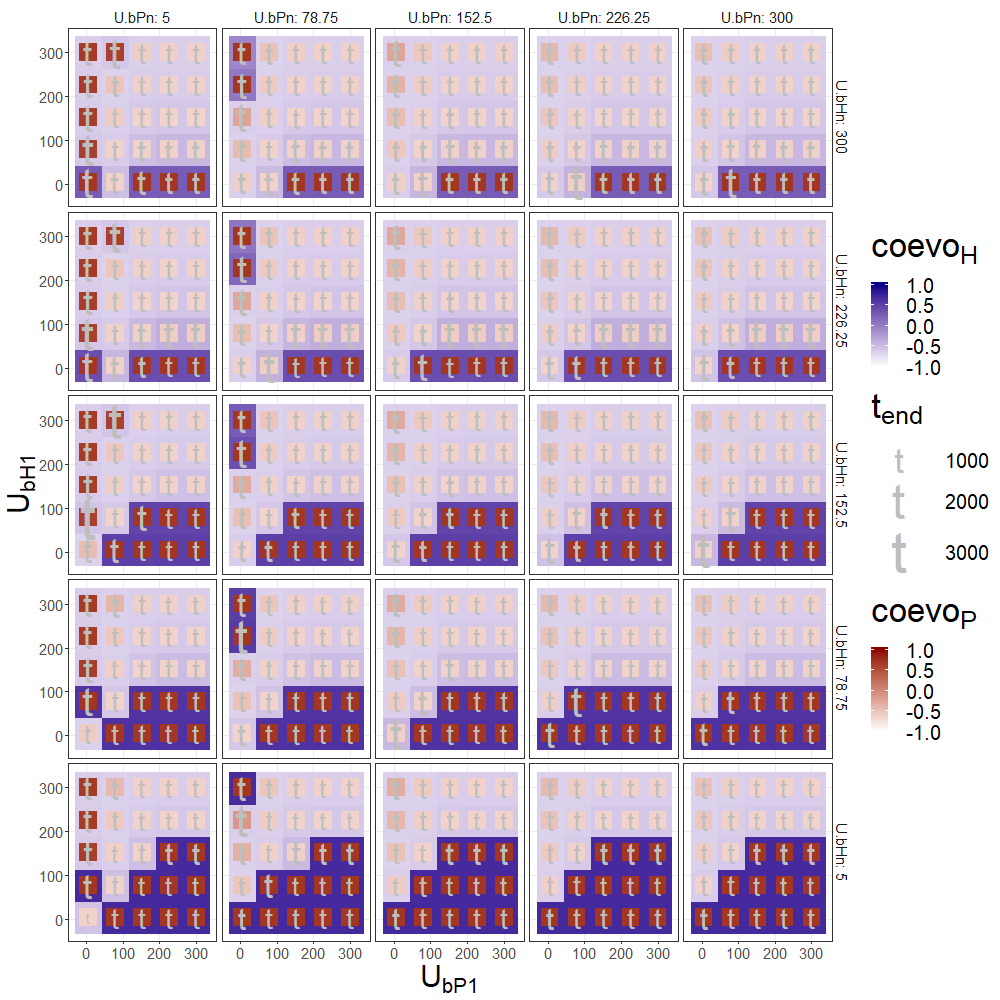
\includegraphics[width=1\linewidth]{plots/4_fourPar-U.bH-U.bP_plot}

\textbf{\emph{Interpretation}}:\\
- Lower values of all four parameters facilitate coevolution; under the `default' setting and for all four parameters, values higher than \(MaxArea\) (here, 200) impede coevolution. The human parameters (\(U_{bH_{1}}\), \(U_{bH_{n}}\)), together regulating the scale of the subsistence alternatives for humans, are significantly more important; their relationship (if one is greater than the other) seems to be less important as long as their combined sum is small enough.\\
* Coevolution is likely to occur when \(U_{bH_{1}}=5\), unless \(U_{bH_{1}}\) is too big and \(U_{bP_{1}}\) is too small.\\
* As a summary of possible end-states:\\
+ \emph{`Fast' coevolution} (red square in blue tile, small \emph{t}): most cases when \(U_{bH_{1}}\) and \(U_{bH_{n}}<152.5\).\\
+ \emph{Domestication without cultivation} (red square in whitish tile): most cases when \(U_{bP_{n}}=5\), \(U_{bP_{1}}=5\) (i.e.~there is very little carrying capacity for plants beyond the anthropic space) and \(U_{bH_{1}}>5\) (i.e.~humans get enough of other resources when -still- not engaged in agriculture).\\
+ \emph{Cultivation without domestication} (whitish square in blue tile): \emph{no cases are visible under these conditions}.

\hypertarget{number-of-types-and-undirected-variation-of-humans-and-plants-n_h-x-n_p-x-v_h-x-v_p}{%
\section{\texorpdfstring{Number of types and undirected variation of humans and plants (\(n_{H}\) x \(n_{P}\) x \(v_{H}\) x \(v_{P}\))}{Number of types and undirected variation of humans and plants (n\_\{H\} x n\_\{P\} x v\_\{H\} x v\_\{P\})}}\label{number-of-types-and-undirected-variation-of-humans-and-plants-n_h-x-n_p-x-v_h-x-v_p}}

\begin{tabular}{l|l}
\hline
parameter & value\\
\hline
iniH & 10\\
\hline
iniP & 10\\
\hline
n.H & 5 - 45 (sample = 5 )\\
\hline
n.P & 5 - 45 (sample = 5 )\\
\hline
v.H & 0.05 - 0.25 (sample = 5 )\\
\hline
v.P & 0.05 - 0.25 (sample = 5 )\\
\hline
r.H & 0.04\\
\hline
r.P & 0.1\\
\hline
mU.PnH & 1.5\\
\hline
mU.HnP & 1\\
\hline
mU.P1H & 0.15\\
\hline
mU.H1P & 0\\
\hline
U.bHn & 10\\
\hline
U.bPn & 20\\
\hline
U.bH1 & 80\\
\hline
U.bP1 & 100\\
\hline
MaxArea & 200\\
\hline
\end{tabular}

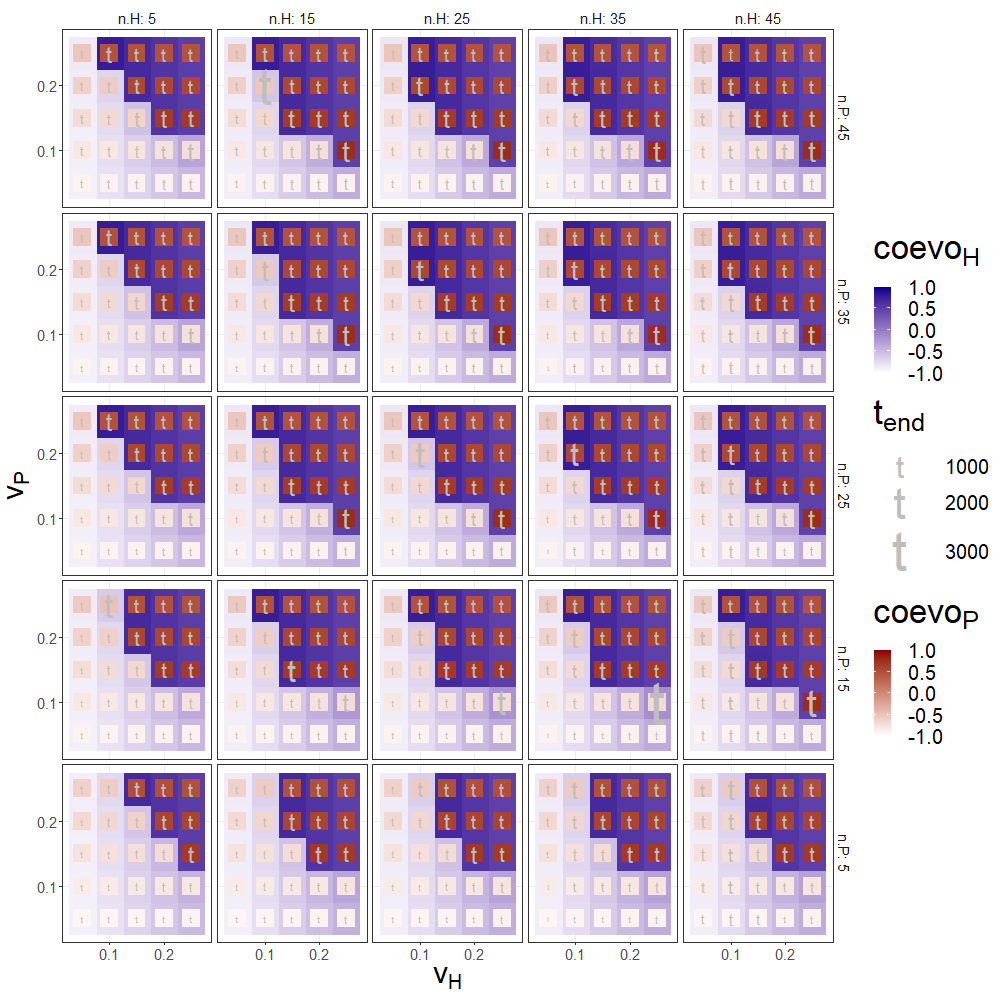
\includegraphics[width=1\linewidth]{plots/4_fourPar-n-v_plot}

\textbf{\emph{Interpretation}}:\\
* Higher values of all four parameters facilitate coevolution. Undirected variation has a stronger effect than number of types.
* As a summary of possible end-states:\\
+ \emph{`Fast' coevolution} (red square in blue tile, small \emph{t}): most cases when the numbers of types (\(n_{H}\), \(n_{P}\)) are greater than \textbf{15} and values of undirected variation (\(v_{H}\), \(v_{P}\)) higher than \textbf{0.15}.\\
+ \emph{`Semi-domestication' without cultivation} (redish square in whitish tile): cases when \(v_{P}\geq 0.15\).\\
+ \emph{`Semi-cultivation' without domestication} (whitish square in blue tile): cases when \(v_{H}\geq 0.15\).

\hypertarget{multiple-parameter-exploration}{%
\chapter{Multiple parameter exploration}\label{multiple-parameter-exploration}}

\hypertarget{sampling-parameter-values-with-latin-hypercube-sampling-lhc}{%
\section{Sampling parameter values with Latin Hypercube Sampling (LHC)}\label{sampling-parameter-values-with-latin-hypercube-sampling-lhc}}

\textbf{\emph{Ranges of parameter exploration}}

\begin{longtable}[]{@{}ll@{}}
\toprule
\textbf{parameter} & \textbf{value}\tabularnewline
\midrule
\endhead
\texttt{n.H}, \texttt{n.P} & {[}3, 50{]}, {[}3, 50{]}\tabularnewline
\texttt{v.H}, \texttt{v.P} & {[}0.1, 0.3{]}, {[}0.1, 0.3{]}\tabularnewline
\texttt{mU.PnH}, \texttt{mU.HnP} & {[}0, 3{]}, {[}0, 3{]}\tabularnewline
\texttt{mU.P1H}, \texttt{mU.H1P} & {[}0, 3{]}, {[}0, 3{]}\tabularnewline
\texttt{U.bH1}, \texttt{U.bP1} & {[}0, 300{]}, {[}0, 300{]}\tabularnewline
\texttt{U.bHn}, \texttt{U.bPn} & {[}0, 300{]}, {[}0, 300{]}\tabularnewline
\bottomrule
\end{longtable}

\textbf{\emph{ACTUAL parameter values}}

\begin{tabular}{l|l}
\hline
parameter & value\\
\hline
n.H & 3 - 50 (sample = 48 )\\
\hline
n.P & 3 - 50 (sample = 48 )\\
\hline
v.H & 0.1 - 0.3 (sample = 7917 )\\
\hline
v.P & 0.10002 - 0.29999 (sample = 7885 )\\
\hline
mU.PnH & 0 - 2.9999 (sample = 8496 )\\
\hline
mU.HnP & 5e-04 - 2.9999 (sample = 8497 )\\
\hline
mU.P1H & 6e-04 - 2.9997 (sample = 8514 )\\
\hline
mU.H1P & 5e-04 - 3 (sample = 8514 )\\
\hline
U.bHn & 0.1479 - 299.931 (sample = 9989 )\\
\hline
U.bPn & 0.0694 - 299.9966 (sample = 9982 )\\
\hline
U.bH1 & 0.028 - 299.9987 (sample = 9978 )\\
\hline
U.bP1 & 0.0336 - 299.991 (sample = 9987 )\\
\hline
\end{tabular}

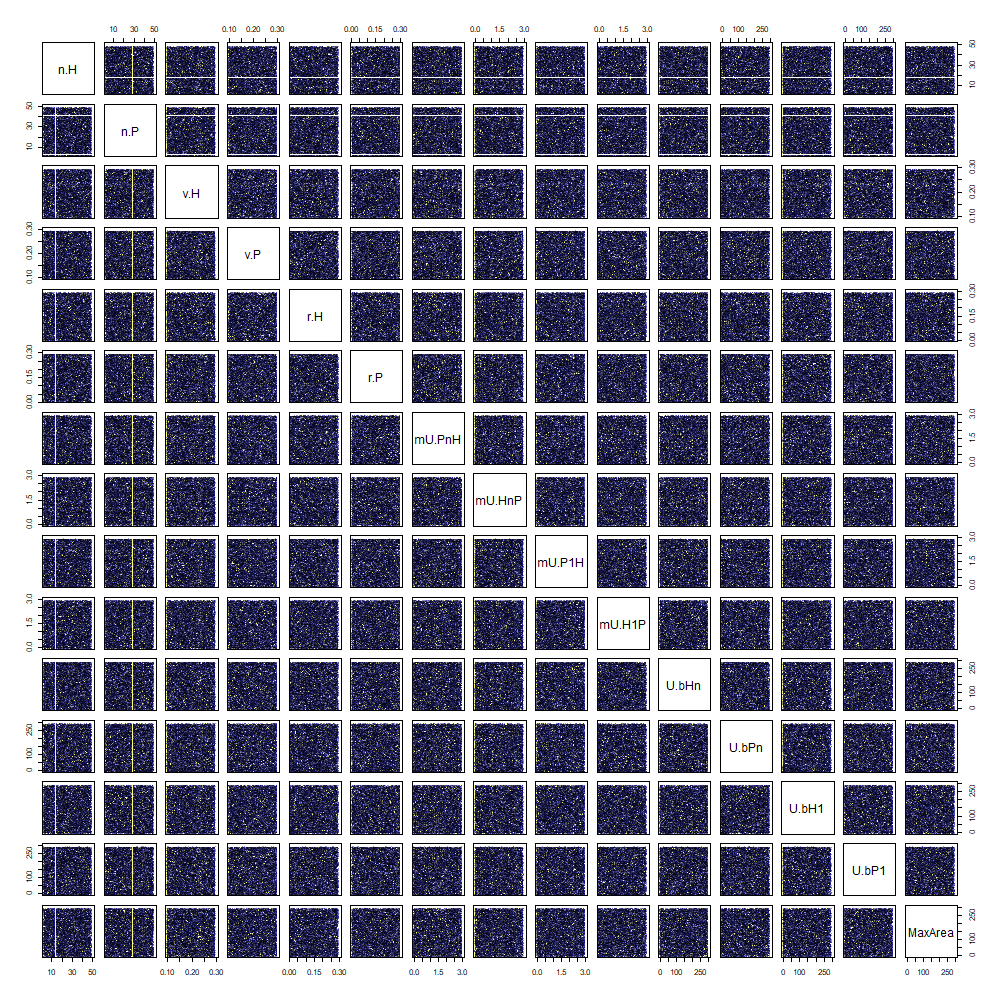
\includegraphics[width=1\linewidth]{plots/5_multiplePar-LHC_pairs-plot}

\hypertarget{experiment-overview}{%
\section{Experiment overview}\label{experiment-overview}}

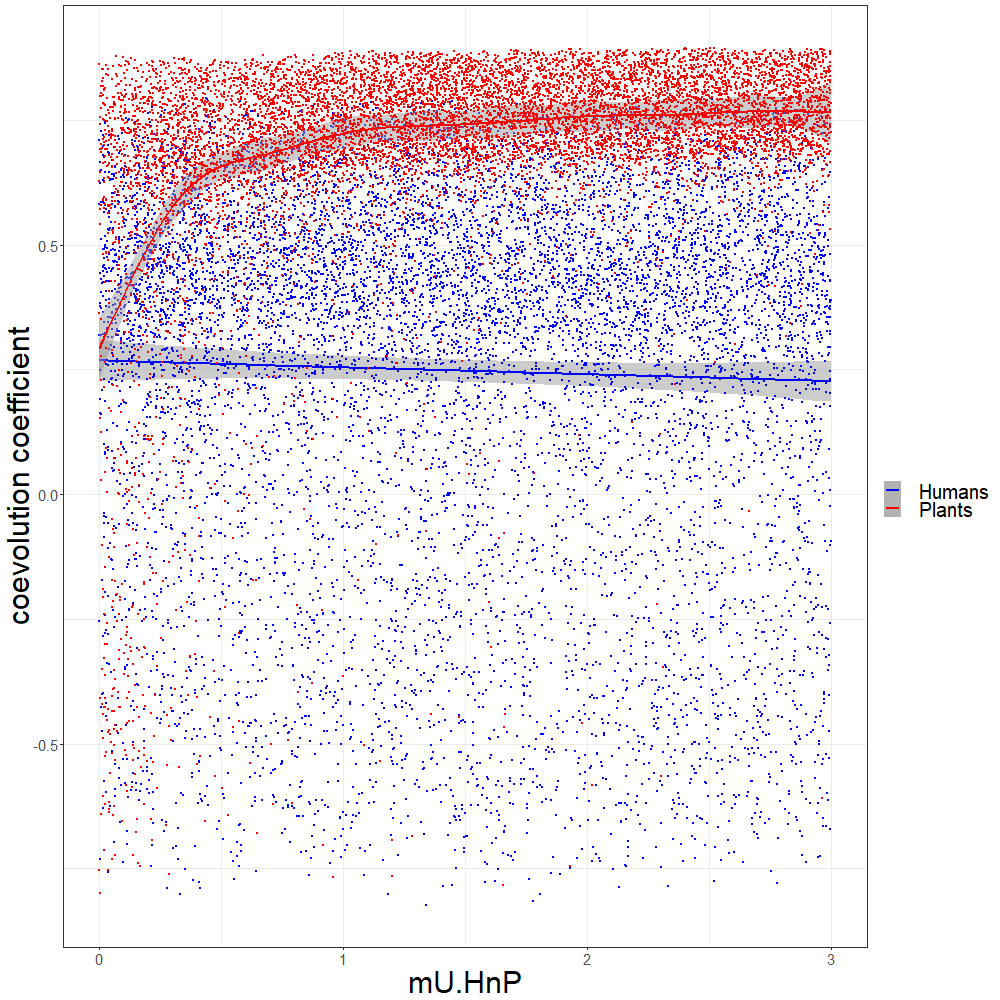
\includegraphics[width=1\linewidth]{plots/5_multiplePar-coevo_collapsed-ggplot}

\hypertarget{random-forest}{%
\subsection{Random forest}\label{random-forest}}

\textbf{\emph{Coevolution coefficients}}

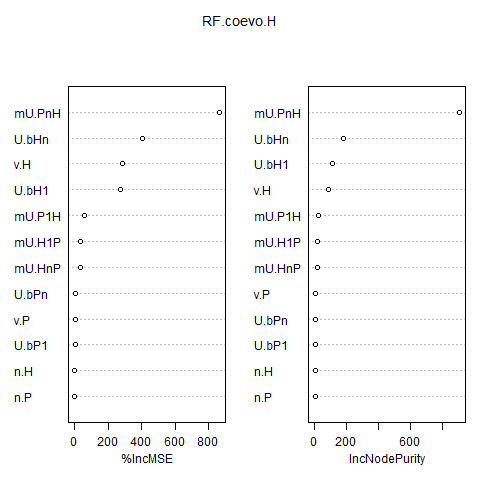
\includegraphics[width=1\linewidth]{plots/5_multiplePar-rf-coevo.H}

\includegraphics[width=1\linewidth]{plots/5_multiplePar-rf-coevo.P}

\textbf{\emph{Dependency coefficients}}

\includegraphics[width=1\linewidth]{plots/5_multiplePar-rf-depend.H}

\includegraphics[width=1\linewidth]{plots/5_multiplePar-rf-depend.P}

\textbf{\emph{Timings}}

\includegraphics[width=1\linewidth]{plots/5_multiplePar-rf-timing.H}

\includegraphics[width=1\linewidth]{plots/5_multiplePar-rf-timing.P}

\hypertarget{scenarios}{%
\section{Scenarios}\label{scenarios}}

\hypertarget{mutualistic-human-type-gives-more-utility-baru_h_np-baru_h_1p}{%
\subsection{\texorpdfstring{Mutualistic human type gives more utility (\(\bar{U}_{H_{n}P}> \bar{U}_{H_{1}P}\))}{Mutualistic human type gives more utility (\textbackslash{}bar\{U\}\_\{H\_\{n\}P\}\textgreater{} \textbackslash{}bar\{U\}\_\{H\_\{1\}P\})}}\label{mutualistic-human-type-gives-more-utility-baru_h_np-baru_h_1p}}

\textbf{\emph{Coevolution coefficients}}

\includegraphics[width=1\linewidth]{plots/5_multiplePar-coevo-humanImprove-ggplot}

\textbf{\emph{Dependency coefficients}}

\includegraphics[width=1\linewidth]{plots/5_multiplePar-depend-humanImprove-ggplot}

\textbf{\emph{Timings}}

\includegraphics[width=1\linewidth]{plots/5_multiplePar-timing-humanImprove-ggplot}

\hypertarget{mutualistic-plant-type-gives-more-utility-baru_p_nh-baru_p_1h}{%
\subsection{\texorpdfstring{Mutualistic plant type gives more utility (\(\bar{U}_{P_{n}H}> \bar{U}_{P_{1}H}\))}{Mutualistic plant type gives more utility (\textbackslash{}bar\{U\}\_\{P\_\{n\}H\}\textgreater{} \textbackslash{}bar\{U\}\_\{P\_\{1\}H\})}}\label{mutualistic-plant-type-gives-more-utility-baru_p_nh-baru_p_1h}}

\textbf{\emph{Coevolution coefficients}}

\includegraphics[width=1\linewidth]{plots/5_multiplePar-coevo-plantImprove-ggplot}

\textbf{\emph{Dependency coefficients}}

\includegraphics[width=1\linewidth]{plots/5_multiplePar-depend-plantImprove-ggplot}

\textbf{\emph{Timings}}

\includegraphics[width=1\linewidth]{plots/5_multiplePar-timing-plantImprove-ggplot}

\hypertarget{mutualistic-types-human-and-plant-give-more-utility-baru_h_np-baru_h_1p-and-baru_p_nh-baru_p_1h}{%
\subsection{\texorpdfstring{Mutualistic types (human and plant) give more utility (\(\bar{U}_{H_{n}P}> \bar{U}_{H_{1}P}\) AND \(\bar{U}_{P_{n}H}> \bar{U}_{P_{1}H}\))}{Mutualistic types (human and plant) give more utility (\textbackslash{}bar\{U\}\_\{H\_\{n\}P\}\textgreater{} \textbackslash{}bar\{U\}\_\{H\_\{1\}P\} AND \textbackslash{}bar\{U\}\_\{P\_\{n\}H\}\textgreater{} \textbackslash{}bar\{U\}\_\{P\_\{1\}H\})}}\label{mutualistic-types-human-and-plant-give-more-utility-baru_h_np-baru_h_1p-and-baru_p_nh-baru_p_1h}}

\textbf{\emph{Coevolution coefficients}}

\includegraphics[width=1\linewidth]{plots/5_multiplePar-coevo-bothImprove-ggplot}

\textbf{\emph{Dependency coefficients}}

\includegraphics[width=1\linewidth]{plots/5_multiplePar-depend-bothImprove-ggplot}

\textbf{\emph{Timings}}

\includegraphics[width=1\linewidth]{plots/5_multiplePar-timing-bothImprove-ggplot}

\hypertarget{mutualistic-human-type-gets-less-utility-from-other-resources-u_bh_1u_bh_n}{%
\subsection{\texorpdfstring{Mutualistic human type gets less utility from other resources (\(U_{bH_{1}}>U_{bH_{n}}\))}{Mutualistic human type gets less utility from other resources (U\_\{bH\_\{1\}\}\textgreater{}U\_\{bH\_\{n\}\})}}\label{mutualistic-human-type-gets-less-utility-from-other-resources-u_bh_1u_bh_n}}

\textbf{\emph{Coevolution coefficients}}

\includegraphics[width=1\linewidth]{plots/5_multiplePar-coevo-humanLessBase-ggplot}

\textbf{\emph{Dependency coefficients}}

\includegraphics[width=1\linewidth]{plots/5_multiplePar-depend-humanLessBase-ggplot}

\textbf{\emph{Timings}}

\includegraphics[width=1\linewidth]{plots/5_multiplePar-timing-humanLessBase-ggplot}

\hypertarget{mutualistic-plant-type-gets-less-utility-from-other-resources-u_bp_1u_bp_n}{%
\subsection{\texorpdfstring{Mutualistic plant type gets less utility from other resources (\(U_{bP_{1}}>U_{bP_{n}}\))}{Mutualistic plant type gets less utility from other resources (U\_\{bP\_\{1\}\}\textgreater{}U\_\{bP\_\{n\}\})}}\label{mutualistic-plant-type-gets-less-utility-from-other-resources-u_bp_1u_bp_n}}

\textbf{\emph{Coevolution coefficients}}

\includegraphics[width=1\linewidth]{plots/5_multiplePar-coevo-plantLessBase-ggplot}

\textbf{\emph{Dependency coefficients}}

\includegraphics[width=1\linewidth]{plots/5_multiplePar-depend-plantLessBase-ggplot}

\textbf{\emph{Timings}}

\includegraphics[width=1\linewidth]{plots/5_multiplePar-timing-plantLessBase-ggplot}

\hypertarget{mutualistic-types-human-and-plant-get-less-utility-from-other-resources-u_bh_1u_bh_n-and-u_bp_1u_bp_n}{%
\subsection{\texorpdfstring{Mutualistic types (human and plant) get less utility from other resources (\(U_{bH_{1}}>U_{bH_{n}}\) AND \(U_{bP_{1}}>U_{bP_{n}}\))}{Mutualistic types (human and plant) get less utility from other resources (U\_\{bH\_\{1\}\}\textgreater{}U\_\{bH\_\{n\}\} AND U\_\{bP\_\{1\}\}\textgreater{}U\_\{bP\_\{n\}\})}}\label{mutualistic-types-human-and-plant-get-less-utility-from-other-resources-u_bh_1u_bh_n-and-u_bp_1u_bp_n}}

\textbf{\emph{Coevolution coefficients}}

\includegraphics[width=1\linewidth]{plots/5_multiplePar-coevo-bothLessBase-ggplot}

\textbf{\emph{Dependency coefficients}}

\includegraphics[width=1\linewidth]{plots/5_multiplePar-depend-bothLessBase-ggplot}

\textbf{\emph{Timings}}

\includegraphics[width=1\linewidth]{plots/5_multiplePar-timing-bothLessBase-ggplot}


\end{document}
